\documentclass[11pt,a4paper]{article}
% ============================================================================
%  TFPT consolidated document --- unified preamble (superset of the merged notes)
% ============================================================================
\usepackage[T1]{fontenc}
\usepackage[utf8]{inputenc}
\usepackage[english]{babel}
\usepackage{lmodern}
\usepackage[a4paper,margin=2.3cm]{geometry}
\usepackage{amsmath,amssymb,amsthm,mathtools}
\usepackage{booktabs,array,longtable,tabularx,multirow}
\usepackage{enumitem}
\usepackage{xcolor}
\usepackage{tikz}
\usetikzlibrary{arrows.meta,positioning,calc,fit,backgrounds,shapes.geometric,shapes.misc,decorations.pathmorphing,decorations.pathreplacing,patterns,angles,quotes,matrix}
\usepackage{microtype}
\usepackage[most]{tcolorbox}
\usepackage[hidelinks,colorlinks=true,linkcolor=blue!55!black,citecolor=blue!55!black,urlcolor=blue!55!black]{hyperref}
\emergencystretch=3.5em

% ---- colours, shared header/footer (version stamp), boxes, markers ----
%  (header/footer and the 4-class markers come from the shared style; no
%   per-document override, so every TFPT document looks identical.)
% ---------------------------------------------------------------------
%  tfpt_style.tex -- THE shared visual style for every TFPT document.
%  Single source for colours, status markers, marker key, the \veri
%  script reference, the tcolorbox families, and the running
%  header/footer.  \input AFTER xcolor + tcolorbox[most] + hyperref are
%  loaded (every paper loads those).  Each document sets its short
%  running title before \begin{document}, e.g.
%        \def\TFPTdoctitle{Architecture and the E8 Compiler}
%  ---------------------------------------------------------------------
\usepackage{fancyhdr}
\usepackage{etoolbox}
\usepackage{tikz}
\usetikzlibrary{positioning,arrows.meta,fit,backgrounds,calc,shapes.geometric,shapes.misc}

% ---- single-source author / version / automatic date stamp ----
% ---------------------------------------------------------------------
%  tex-artefacts/version.tex -- single source for author list, version
%  and the automatic title-page date stamp of every TFPT document.
%  \input by tex-artefacts/tfpt_style.tex, so every paper that loads the
%  shared style automatically gets:
%     \TFPTauthors   -- the author list (use as \author{\TFPTauthors})
%     \TFPTversion   -- curated semantic version (bump per release; mirror
%                       the bump in changelog.tex)
%     \TFPTrev       -- auto build revision = git commit count, injected by
%                       build.sh into tex-artefacts/version-auto.tex
%                       (gitignored); falls back to "dev" for standalone runs
%     \TFPTdatestamp -- the title-page date line: \today + version + revision
%  build.sh also writes tex-artefacts/release-version.txt (gitignored):
%     "{TFPTversion} (rev {git commit count})" for Zenodo + release tooling.
%  Bump \TFPTversion here ONCE; it then updates in all papers at the next build.
% ---------------------------------------------------------------------
\def\TFPTauthors{Stefan Hamann \and Alessandro Rizzo}
\def\TFPTversion{5.3}
\def\TFPTrev{dev}
% build.sh regenerates the line below with the live git commit count:
\InputIfFileExists{tex-artefacts/version-auto.tex}{}{}
\def\TFPTdatestamp{\today\,\textperiodcentered\,v\TFPTversion\,(rev~\TFPTrev)}


% ---- colours (canonical TFPT palette) ----
\definecolor{tfblue}{HTML}{1F4E79}
\definecolor{tfgreen}{HTML}{1E7B45}
\definecolor{tfred}{HTML}{9B2226}
\definecolor{tfgold}{HTML}{B8860B}
\definecolor{tfgray}{HTML}{555555}

% ---- status markers (simplified 4-class display system) ----
% Reader-facing markers collapse to FOUR classes.  The fine-grained per-claim
% type (Axiom / Formal / Lattice / Numerical / Identity / Physical) stays in
% verification/status_ledger.csv -- the single source of truth -- so no fidelity
% is lost; the papers just show the coarse class so a reader is not overwhelmed.
%   [E] exact / machine-proven  (identity, Lie/lattice, formalised, numerical FP)
%   [C] conditional             (physical / bridge / readout, under named hypotheses)
%   [O] open / axiom            (declared input or genuine gap)
%   [X] kill test               (falsifiable threshold)
\newcommand{\mE}{{\small\textcolor{tfgreen!70!black}{\textbf{[E]}}}}
\newcommand{\mC}{{\small\textcolor{tfgold!78!black}{\textbf{[C]}}}}
\newcommand{\mO}{{\small\textcolor{tfred!80!black}{\textbf{[O]}}}}
\newcommand{\mX}{{\small\textcolor{tfred!58!black}{\textbf{[X]}}}}
% backward-compatible aliases: the old fine-grained names now render their class,
% so any not-yet-rewritten call site (or the standalone changelog) still compiles.
\newcommand{\tI}{\mE}\newcommand{\tL}{\mE}\newcommand{\tF}{\mE}\newcommand{\tN}{\mE}
\newcommand{\tIalg}{\mE}\newcommand{\tInum}{\mE}
\newcommand{\tP}{\mC}\newcommand{\tB}{\mC}\newcommand{\tR}{\mC}
\newcommand{\tA}{\mO}
\newcommand{\tX}{\mX}

% compact marker legend, placed under a marker-bearing table
\newcommand{\markerkey}{\par\vspace{1.5pt}\noindent{\scriptsize\itshape
  \textcolor{black!58}{Marker key:\ \mE~exact / machine-proven\,$\cdot$\,%
  \mC~conditional (holds under named hypotheses)\,$\cdot$\,%
  \mO~open / axiom\,$\cdot$\,\mX~falsifiable kill test.\ \
  Per-claim fine type in \texttt{verification/status\_ledger.csv}.}}\par\vspace{2pt}}

% horizontal badge bar (place once near the front of a document)
\newcommand{\TFPTbadges}{\par\noindent
  \fcolorbox{tfgreen!55!black}{tfgreen!8}{\scriptsize\mE\,exact / machine-proven}\hfill
  \fcolorbox{tfgold!70!black}{tfgold!10}{\scriptsize\mC\,conditional}\hfill
  \fcolorbox{tfred!75!black}{tfred!8}{\scriptsize\mO\,open / axiom}\hfill
  \fcolorbox{tfred!60!black}{tfred!6}{\scriptsize\mX\,kill test}\par\vspace{3pt}}

% inline reference to the script that machine-checks a claim (see verification/)
\newcommand{\veri}[1]{\,{\footnotesize\textcolor{tfblue!70!black}{[\,\texttt{verification/#1}\,]}}}
% lightweight inline colour-mark for a bare verification-script token in running
% prose / tables, e.g. \vref{v108}, \vref{v49}/\vref{v71}.  Same blue as \veri so a
% reader instantly sees "this is a machine-checked module reference".
\newcommand{\vref}[1]{\textcolor{tfblue!72!black}{\textsf{#1}}}

% ---- tcolorbox families (one visual language across all documents) ----
% keybox  : the central claim / reading of a section (blue)
% winbox  : an established result / closure (green)
% gapbox  : an open gate / honest caveat / kill criterion (red)
% auditbox: a recorded audit fingerprint, not load-bearing (gold)
% navbox  : a light, neutral navigation / reference card (document map, etc.)
% Visual language (deliberately light): a faint tint, a thin coloured frame
% and a light title band with dark coloured title text -- NOT a heavy
% white-on-saturated-colour bar -- so a page never reads as a wall of boxes.
\newtcolorbox{keybox}[1][]{enhanced,breakable,boxrule=0.5pt,arc=1.5pt,
  colback=tfblue!4!white,colframe=tfblue!70!black,coltitle=tfblue!88!black,colbacktitle=tfblue!12!white,
  fonttitle=\bfseries\small,fontupper=\small,title={#1},left=2mm,right=2mm,top=1mm,bottom=1mm}
% non-breaking variant (front-matter cards that should never split across a page)
\newtcolorbox{keyboxnb}[1][]{enhanced,breakable=false,boxrule=0.5pt,arc=1.5pt,
  colback=tfblue!4!white,colframe=tfblue!70!black,coltitle=tfblue!88!black,colbacktitle=tfblue!12!white,
  fonttitle=\bfseries\small,fontupper=\small,title={#1},left=2mm,right=2mm,top=1mm,bottom=1mm}
\newtcolorbox{winbox}[1][]{enhanced,breakable,boxrule=0.5pt,arc=1.5pt,
  colback=tfgreen!5!white,colframe=tfgreen!65!black,coltitle=tfgreen!50!black,colbacktitle=tfgreen!14!white,
  fonttitle=\bfseries\small,fontupper=\small,title={#1},left=2mm,right=2mm,top=1mm,bottom=1mm}
\newtcolorbox{gapbox}[1][]{enhanced,breakable,boxrule=0.5pt,arc=1.5pt,
  colback=tfred!4!white,colframe=tfred!70!black,coltitle=tfred!75!black,colbacktitle=tfred!12!white,
  fonttitle=\bfseries\small,fontupper=\small,title={#1},left=2mm,right=2mm,top=1mm,bottom=1mm}
% non-breaking variants (callouts that must stay whole on one page, embedded in text)
\newtcolorbox{winboxnb}[1][]{enhanced,breakable=false,boxrule=0.5pt,arc=1.5pt,
  colback=tfgreen!5!white,colframe=tfgreen!65!black,coltitle=tfgreen!50!black,colbacktitle=tfgreen!14!white,
  fonttitle=\bfseries\small,fontupper=\small,title={#1},left=2mm,right=2mm,top=1mm,bottom=1mm}
\newtcolorbox{gapboxnb}[1][]{enhanced,breakable=false,boxrule=0.5pt,arc=1.5pt,
  colback=tfred!4!white,colframe=tfred!70!black,coltitle=tfred!75!black,colbacktitle=tfred!12!white,
  fonttitle=\bfseries\small,fontupper=\small,title={#1},left=2mm,right=2mm,top=1mm,bottom=1mm}
\newtcolorbox{auditbox}[1][]{enhanced,breakable,boxrule=0.5pt,arc=1.5pt,
  colback=tfgold!7!white,colframe=tfgold!70!black,coltitle=tfgold!45!black,colbacktitle=tfgold!16!white,
  fonttitle=\bfseries\small,fontupper=\small,title={#1},left=2mm,right=2mm,top=1mm,bottom=1mm}
\newtcolorbox{navbox}[1][]{enhanced,breakable,boxrule=0.5pt,arc=1.5pt,
  colback=tfgray!3!white,colframe=tfgray!55,coltitle=tfgray!30!black,colbacktitle=tfgray!12!white,
  fonttitle=\bfseries\small,fontupper=\small,title={#1},left=2mm,right=2mm,top=1mm,bottom=1mm}
% back-compatibility aliases (older box names map onto the canonical types)
\newtcolorbox{audbox}[1][]{enhanced,breakable,boxrule=0.5pt,arc=1.5pt,
  colback=tfgold!7!white,colframe=tfgold!70!black,coltitle=tfgold!45!black,colbacktitle=tfgold!16!white,
  fonttitle=\bfseries\small,fontupper=\small,title={#1},left=2mm,right=2mm,top=1mm,bottom=1mm}
\newtcolorbox{resbox}[1][]{enhanced,breakable,boxrule=0.5pt,arc=1.5pt,
  colback=tfgreen!5!white,colframe=tfgreen!55!black,coltitle=tfgreen!50!black,colbacktitle=tfgreen!12!white,
  fonttitle=\bfseries\small,fontupper=\small,title={#1},left=2mm,right=2mm,top=1mm,bottom=1mm}
\newtcolorbox{roadbox}[1][]{enhanced,breakable,boxrule=0.5pt,arc=1.5pt,
  colback=tfgreen!5!white,colframe=tfgreen!55!black,coltitle=tfgreen!50!black,colbacktitle=tfgreen!12!white,
  fonttitle=\bfseries\small,fontupper=\small,title={#1},left=2mm,right=2mm,top=1mm,bottom=1mm}
\newtcolorbox{intbox}[1][]{enhanced,breakable,boxrule=0.5pt,arc=1.5pt,
  colback=tfgold!7!white,colframe=tfgold!70!black,coltitle=tfgold!45!black,colbacktitle=tfgold!16!white,
  fonttitle=\bfseries\small,fontupper=\small,title={#1},left=2mm,right=2mm,top=1mm,bottom=1mm}

% ---- colour-marked display formula (load-bearing key equations) ----
% A highlighted formula line: a coloured left accent bar + faint tint, no full
% frame -- so a key equation is visually set apart from the running prose
% without becoming yet another box.  Use:  \begin{keyeq}$\displaystyle ...$\end{keyeq}
\newtcolorbox{keyeq}{blanker,breakable=false,halign=center,
  colback=tfgold!8!white,borderline west={2.4pt}{0pt}{tfgold!75!black},
  left=8pt,right=6pt,top=3pt,bottom=3pt,before skip=5pt,after skip=5pt}

% ---- running header / footer (consistent across all documents) ----
\providecommand{\TFPTdoctitle}{}
\setlength{\headheight}{14pt}
\pagestyle{fancy}
\fancyhf{}
\fancyhead[L]{\footnotesize\textcolor{tfgray}{\textit{TFPT}\,\textbullet\,\TFPTdoctitle}}
\fancyhead[R]{\footnotesize\textcolor{tfgray}{\thepage}}
\fancyfoot[L]{\scriptsize\textcolor{tfgray}{v\TFPTversion\,\textperiodcentered\,rev~\TFPTrev}}
\renewcommand{\headrulewidth}{0.3pt}
\renewcommand{\footrulewidth}{0pt}
\fancypagestyle{plain}{\fancyhf{}\renewcommand{\headrulewidth}{0pt}%
  \fancyfoot[C]{\footnotesize\textcolor{tfgray}{\thepage}}%
  \fancyfoot[L]{\scriptsize\textcolor{tfgray}{v\TFPTversion\,\textperiodcentered\,rev~\TFPTrev}}}

% ---- shared figure macros (claim stack, anchor cockpit, E8 glue, 2/3 motif, K5) ----
%  (this fragment lives in tex-artefacts/ and is \input by documents compiled from
%   the repository root, so the path is given relative to that root.)
% ---------------------------------------------------------------------
%  tfpt_figures.tex -- shared, reusable TikZ figure macros for every
%  TFPT document.  \input by tfpt_style.tex (which loads tikz + the
%  needed libraries + etoolbox).  Each macro draws a self-contained
%  centred figure; nothing is drawn until the macro is called.
%
%    \TFPTclaimstack[zone]  -- the architecture claim stack (B3); the
%                              optional zone in {axioms,anchor,compiler,
%                              sm,bridges,frontier} is highlighted.
%    \TFPTanchorcockpit      -- the anchor a=(1,1,2) cockpit (B4)
%    \TFPTeightglue          -- the D5 (+) A3 +mu4 => E8 glue (B5)
%    \TFPTmotif              -- the 2/3 motif map (B6)
%    \TFPTactionkfive        -- the K5 action-lattice mnemonic (B7)
% ---------------------------------------------------------------------

% ===== B3: the architecture claim stack =========================
\newcommand{\tfhl}[1]{\ifdefstring{\tfcur}{#1}{cbhi}{cbnl}}
\newcommand{\TFPTclaimstack}[1][none]{%
\def\tfcur{#1}%
\begin{center}
\begin{tikzpicture}[font=\footnotesize,
  cb/.style={rounded corners=2pt,inner sep=4pt,text width=118mm,align=center,minimum height=8.5mm},
  cbnl/.style={line width=0.5pt}, cbhi/.style={line width=1.5pt},
  ar/.style={-{Stealth[length=2.2mm]},tfgray,semithick}]
  \node[cb,fill=tfred!8,draw=tfred!75!black,\tfhl{axioms}] (axioms)
    {\textbf{P1}\,$c_3=\tfrac1{8\pi}$ \quad \textbf{P2}\,$g_{\mathrm{car}}=5$ \ \textcolor{tfgray}{\itshape(two inputs, [O] axioms)}};
  \node[cb,fill=tfblue!8,draw=tfblue,\tfhl{anchor},below=3.5mm of axioms] (anchor)
    {Anchor $a=(1,1,2)$:\ $e_1,e_2,e_3=4,5,2$ \ \textcolor{tfgray}{\itshape([E] exact)}};
  \node[cb,fill=tfgreen!10,draw=tfgreen!70!black,\tfhl{compiler},below=3.5mm of anchor] (compiler)
    {Discrete compiler:\ $D_5\oplus A_3+\mu_4\Rightarrow E_8$,\ $h=30$,\ $\varphi_0$ \ \textcolor{tfgray}{\itshape([E] exact)}};
  \node[cb,fill=tfgreen!7,draw=tfgreen!60!black,\tfhl{sm},below=3.5mm of compiler] (sm)
    {SM skeleton:\ three families, hypercharges, flavor matrix $R$ \ \textcolor{tfgray}{\itshape([E])}};
  \node[cb,fill=tfgold!12,draw=tfgold!80!black,\tfhl{bridges},below=3.5mm of sm] (bridges)
    {Physical bridges:\ $v_{\mathrm{geo}}$,\ $G_{\mathrm{net}}$,\ $F_{\mathrm{transfer}}$ \ \textcolor{tfgray}{\itshape([C] bridges)}};
  \node[cb,fill=tfgray!12,draw=tfgray!70!black,\tfhl{frontier},below=3.5mm of bridges] (frontier)
    {Frontier readouts:\ $\Lambda$, inflation, $\eta_B$, dark matter, QG \ \textcolor{tfgray}{\itshape([C]/[O])}};
  \draw[ar] (axioms)--(anchor); \draw[ar] (anchor)--(compiler);
  \draw[ar] (compiler)--(sm);   \draw[ar] (sm)--(bridges); \draw[ar] (bridges)--(frontier);
\end{tikzpicture}
\end{center}}

% ===== B4: the anchor cockpit ====================================
\newcommand{\TFPTanchorcockpit}{%
\begin{center}
\begin{tikzpicture}[font=\footnotesize,
  pan/.style={rounded corners=2pt,draw=tfblue!60,fill=tfblue!4,inner sep=5pt,
    text width=46mm,align=left},
  hd/.style={font=\bfseries\small,tfblue}]
  \node[pan] (e) {\textbf{elementary} $e_k(a)$\\[2pt]
     $e_1=4\to|\mu_4|$\\ $e_2=5\to g_{\mathrm{car}}$\\ $e_3=2\to|\mathbb Z_2|$\\[2pt]
     $c_3=\tfrac1{2e_1\pi}=\tfrac1{8\pi}$};
  \node[pan,right=4mm of e] (p) {\textbf{power sums} $p_n=2+2^n$\\[2pt]
     $p_0,p_1,p_2,p_3=3,4,6,10$\\ $p_1p_2p_3=240=|R(E_8)|$\\ $p_4-p_3=8=\operatorname{rank}E_8$\\
     $\Rightarrow\dim E_8=248$};
  \node[pan,right=4mm of p] (m) {\textbf{derived motifs}\\[2pt]
     $4,5,8,16,25,$\\ $30,41,120,240$\\[2pt]
     \textcolor{tfgray}{\itshape one anchor,}\\ \textcolor{tfgray}{\itshape many projections}};
  \node[hd,above=1mm of p.north] {$a=(1,1,2)$ \ \textcolor{tfgray}{\footnotesize\itshape[E]}};
\end{tikzpicture}
\end{center}}

% ===== B5: the E8 glue ===========================================
\newcommand{\TFPTeightglue}{%
\begin{center}
\begin{tikzpicture}[font=\footnotesize,
  d/.style={rounded corners=2pt,draw=tfblue,fill=tfblue!6,inner sep=4pt,align=center,text width=36mm},
  mid/.style={rounded corners=2pt,draw=tfgold!80!black,fill=tfgold!12,inner sep=4pt,align=center,text width=52mm},
  e8/.style={rounded corners=2pt,draw=tfgreen!70!black,fill=tfgreen!10,inner sep=4pt,align=center,text width=52mm,font=\bfseries},
  rt/.style={rounded corners=2pt,draw=tfgreen!55!black,fill=tfgreen!6,inner sep=3pt,align=center,text width=52mm},
  side/.style={rounded corners=2pt,draw=tfgray!55,fill=tfgray!6,inner sep=4pt,align=left,text width=34mm,font=\scriptsize},
  ar/.style={-{Stealth[length=2mm]},tfgray,semithick}]
  \node[d] (d5) {$D_5$ discriminant\\ $\mathbb Z_4$, $q=5/4$};
  \node[d,right=10mm of d5] (a3) {$A_3$ discriminant\\ $\mathbb Z_4$, $q=3/4$};
  \node[mid,below=5mm of $(d5)!0.5!(a3)$] (glue) {$\mu_4$ anti-isometry\ ($q$-sum $=2$)};
  \node[e8,below=4mm of glue] (e8) {even unimodular $E_8$ lattice};
  \node[rt,below=4mm of e8] (rt) {$240$ roots,\ rank $8$,\ $\dim=248$};
  \node[side,right=8mm of glue] (why) {\textbf{why unique?}\\ rank $8$\\ even\\ unimodular\\ positive definite};
  \draw[ar] (d5)--(glue); \draw[ar] (a3)--(glue);
  \draw[ar] (glue)--(e8); \draw[ar] (e8)--(rt);
\end{tikzpicture}\\[2pt]
{\scriptsize\itshape $D_5\oplus A_3+\mu_4\Rightarrow E_8$ --- the unique even unimodular rank-$8$ glue \ [E] exact (lattice).}
\end{center}}

% ===== B5b: the double pushout (one glue, two categories) ========
\newcommand{\TFPTdoublepushout}{%
\begin{center}
\begin{tikzpicture}[font=\footnotesize,>={Stealth[length=2mm]},
  lat/.style={rounded corners=2pt,draw=tfblue,fill=tfblue!6,inner sep=5pt,align=center,text width=34mm},
  net/.style={rounded corners=2pt,draw=tfblue!70!black,fill=tfblue!4,inner sep=5pt,align=center,text width=34mm},
  e8l/.style={rounded corners=2pt,draw=tfgold!80!black,fill=tfgold!12,inner sep=5pt,align=center,text width=34mm,font=\bfseries},
  e8n/.style={rounded corners=2pt,draw=tfgreen!70!black,fill=tfgreen!10,inner sep=5pt,align=center,text width=34mm,font=\bfseries},
  ar/.style={->,tfgray,semithick},
  lb/.style={font=\scriptsize,text=black,align=center,fill=white,inner sep=1.5pt}]
  \node[lat] (LL) at (0,2.5)   {$D_5\oplus A_3$\\[1pt]\scriptsize root lattices,\ $\mathrm{disc}=\Z_4$};
  \node[e8l] (LR) at (6.6,2.5) {$E_8$\\[1pt]\scriptsize even unimodular,\ $\det 1$};
  \node[net] (BL) at (0,0)     {$(D_5)_1\otimes(A_3)_1$\\[1pt]\scriptsize chiral nets,\ $c=8$};
  \node[e8n] (BR) at (6.6,0)   {$(E_8)_1$\\[1pt]\scriptsize holomorphic,\ $\mu$-index $1$};
  \draw[ar] (LL)--node[lb]{$+\,\mu_4$ glue}(LR);
  \draw[ar] (BL)--node[lb]{$\rtimes\,\mu_4$ extension}(BR);
  \draw[ar] (LL)--node[lb,left=-1pt]{level-$1$}(BL);
  \draw[ar] (LR)--node[lb,right=-1pt]{level-$1$}(BR);
\end{tikzpicture}\\[2pt]
{\scriptsize\itshape One operation, two categories: the order-$|\mu_4|{=}4$ glue is the lattice pushout
$D_5\oplus A_3+\mu_4\Rightarrow E_8$ \emph{and} the simple-current / anyon-condensation extension
$(D_5)_1\otimes(A_3)_1\rtimes\mu_4\cong(E_8)_1$; the square commutes. \ [E] exact.}
\end{center}}

% ===== B6: the 2/3 motif map =====================================
\newcommand{\TFPTmotif}{%
\begin{center}
\begin{tikzpicture}[font=\footnotesize,
  ex/.style={rounded corners=2pt,draw=tfgreen!70!black,fill=tfgreen!8,inner sep=4pt,align=center,text width=92mm},
  br/.style={rounded corners=2pt,draw=tfgold!80!black,fill=tfgold!12,inner sep=4pt,align=center,text width=92mm},
  ar/.style={-{Stealth[length=2mm]},tfgray,semithick}]
  \node[ex] (a) {$|\mathbb Z_2|/N_{\mathrm{fam}}=2/3$ \ \textcolor{tfgray}{\itshape(anchor ratio)}};
  \node[ex,below=3mm of a] (b) {parabolic weights $\{0,\tfrac13,\tfrac23\}=\operatorname{spec}A_0^\star$};
  \node[ex,below=3mm of b] (c) {transfer spectrum $\{1,(2/3)^6,(1/3)^6\}$,\ gap $6\log\tfrac32$};
  \node[br,below=3mm of c] (d) {Koide target $2/3$ \ \textcolor{tfgray}{\itshape(source$\to$pole bridge [C])}};
  \node[br,below=3mm of d] (e) {Nariai / horizon entropy bound $2/3$ \ \textcolor{tfgray}{\itshape([C])}};
  \draw[ar] (a)--(b); \draw[ar] (b)--(c); \draw[ar] (c)--(d); \draw[ar] (d)--(e);
\end{tikzpicture}\\[2pt]
{\scriptsize\itshape Green: exact motif ([E]).\quad Gold: physical bridge ([C]) --- the same ratio, two epistemic types.}
\end{center}}

% ===== B7: the K5 action-lattice mnemonic ========================
%  Layout: complete graph K5 (pentagon, all 10 edges) on the LEFT, the
%  Pascal-row reading list on the RIGHT, vertically centred on the graph
%  so the two blocks never overlap.
\newcommand{\TFPTactionkfive}{%
\begin{center}
\begin{tikzpicture}[font=\scriptsize]
  % --- K5 vertices on a regular pentagon, centred at the origin ---
  \foreach \i in {1,...,5}{\coordinate (k\i) at ({90+72*(\i-1)}:12mm);}
  \begin{scope}[on background layer]
    \foreach \i in {1,...,5}{\foreach \j in {1,...,5}{\ifnum\i<\j
      \draw[tfgray!55,line width=0.5pt] (k\i)--(k\j);\fi}}
  \end{scope}
  \foreach \i in {1,...,5}{\fill[tfblue!70!black] (k\i) circle (1.8pt);}
  \node[tfgray,font=\scriptsize\itshape] at (0,-1.9) {$K_5$};
  % --- reading list, anchored to the right of the whole graph, centred ---
  \node[anchor=west,align=left,inner sep=0pt] at (1.9cm,0) {%
    $\tbinom51=5$\ \ vertices --- action $x^1$ (Hubble slot)\\[1pt]
    $\tbinom52=10$\ edges --- $\Lambda$ density pair $x^{10}$\\[1pt]
    $\tbinom53=10$\ triangles --- dual sector\\[1pt]
    $\tbinom54=5$\ \ complements --- inverse sector\\[1pt]
    $\tbinom55=1$\ \ determinant --- closure};
\end{tikzpicture}\\[2pt]
{\scriptsize\itshape $K_5$ on the five carrier slots; the action powers $x^{1},x^{5},x^{10}$ are its
$\tbinom5k$ faces \ \textcolor{tfgray}{(mnemonic; the physical scale map stays [C]).}}
\end{center}}



% ---- symbol macros (union; one definition each) ----
\newcommand{\TFPT}{\mathrm{TFPT}}
\newcommand{\MPl}{M_{\mathrm{Pl}}}
\newcommand{\Mpl}{M_{\mathrm{Pl}}}
\newcommand{\Mbar}{\bar M_{\mathrm{Pl}}}
\newcommand{\ellbar}{\bar\ell_{\mathrm{Pl}}}
\newcommand{\GN}{G_N}
\newcommand{\gcar}{g_{\mathrm{car}}}
\newcommand{\Nfam}{N_{\mathrm{fam}}}
\newcommand{\Oadm}{\Omega_{\mathrm{adm}}}
\newcommand{\cthree}{c_3}
\newcommand{\phiz}{\varphi_0^{\mathrm{ret}}}
\newcommand{\phibase}{\varphi_{\mathrm{base}}}
\newcommand{\phiseam}{\varphi_{\mathrm{seam}}}
\newcommand{\useed}{u}
\newcommand{\dtop}{\delta_{\mathrm{top}}}
\newcommand{\dtwo}{\delta_2}
\newcommand{\dph}{\delta_{\mathrm{ph}}}
\newcommand{\betarad}{\beta_{\mathrm{rad}}}
\newcommand{\lC}{\lambda_C}
\newcommand{\lamC}{\lambda_C}
\newcommand{\ainv}{\alpha^{-1}_\star}
\newcommand{\LamIR}{\Lambda_{\mathrm{IR}}}
\newcommand{\Lamgeom}{\Lambda_{\mathrm{geom}}}
\newcommand{\lamsig}{\lambda_\Sigma}
\newcommand{\AEW}{A_{\mathrm{EW}}}
\newcommand{\AL}{\mathcal A_\Lambda}
\newcommand{\AH}{\mathcal A_H}
\newcommand{\dimg}{\dim\mathfrak g_{\mathrm{SM}}}
\newcommand{\Dstart}{D_{\mathrm{start}}}
\newcommand{\kappaE}{\kappa_{E_8}}
\newcommand{\PP}{\mathbb{P}}
\newcommand{\Z}{\mathbb{Z}}
\newcommand{\onev}{\mathbf 1}
\newcommand{\lambdaY}{\lambda_Y}
\newcommand{\lamY}{\lambda_Y}
\newcommand{\vgeo}{v_{\mathrm{geo}}}
\newcommand{\pardeg}{\operatorname{pardeg}}

% ---- theorem environments (union) ----
\theoremstyle{definition}
\newtheorem{theorem}{Theorem}
\newtheorem{proposition}{Proposition}
\newtheorem{lemma}{Lemma}
\newtheorem{corollary}{Corollary}
\newtheorem{conjecture}{Conjecture}
\newtheorem{definition}{Definition}
\newtheorem*{remark}{Remark}
\newtheorem*{goal}{Project goal}

% ---- table column types ----
\newcolumntype{Y}{>{\raggedright\arraybackslash}X}
\newcolumntype{C}{>{\centering\arraybackslash}X}

% ---- list spacing ----
\setlist[itemize]{topsep=4pt,itemsep=2pt,parsep=0pt}
\setlist[enumerate]{topsep=4pt,itemsep=2pt,parsep=0pt}

% ---- TikZ styles used by the architecture diagrams ----
\tikzset{
  cbox/.style={rounded corners=2pt, draw=blue!55!black, fill=blue!6, line width=0.6pt, align=center, inner sep=4pt, font=\small},
  dbox/.style={rounded corners=2pt, draw=teal!60!black, fill=teal!8, line width=0.6pt, align=center, inner sep=4pt, font=\small},
  abox/.style={rounded corners=2pt, draw=orange!70!black, fill=orange!10, line width=0.6pt, align=center, inner sep=4pt, font=\small},
  ebox/.style={rounded corners=2pt, draw=purple!60!black, fill=purple!8, line width=0.8pt, align=center, inner sep=5pt, font=\small\bfseries},
  flow/.style={-{Stealth[length=2.4mm]}, line width=0.7pt, draw=black!65},
}
\renewcommand{\arraystretch}{1.15}

\title{\vspace{-1.2cm}\textbf{TFPT --- Architecture and the $E_8$ Compiler}\\[2mm]\large The two axioms $\{c_3,g_{\mathrm{car}}\}$, the derivation map, and the Coxeter--cyclotomic $D_5\times A_3\to E_8$ construction}
\author{\TFPTauthors}\date{\TFPTdatestamp}
\def\TFPTdoctitle{Architecture \& the $E_8$ Compiler}
\begin{document}
\maketitle
\vspace{-0.4cm}

\begin{keybox}[What this document is about]
The architecture layer: how the two axioms $c_3=\tfrac1{8\pi}$ and $g_{\mathrm{car}}=5$ build the
Coxeter--cyclotomic compiler --- the carrier $C^+{=}D_5$, the family geometry $\mathbb P^1\setminus\mu_4{=}A_3$,
the $\mu_4$ glue $D_5\oplus A_3+\mu_4\Rightarrow E_8$, the EM fixed point $\alpha^{-1}$ (with its ablation),
and the whole number alphabet $16,40,41,48,240,248$ as carrier traces.
\end{keybox}

% ---------------------------------------------------------------------
%  tfpt_docset.tex -- THE canonical TFPT document-set box.
%  Single source of truth for the document list; \input by the
%  introduction and every paper. Uses only universally available
%  macros (keybox + plain LaTeX math) so it compiles in every doc.
%  Each document adds its own "You are reading ..." line directly
%  after the \input.  Numbering is aligned with the file names:
%  document N == tfpt_N_*, the introduction is the entry point, and
%  R/H/O are the appendix-style companions.
% ---------------------------------------------------------------------
\begin{navbox}[The TFPT document set --- what is treated where]
\textbf{Plain language:} TFPT (Topological Fixed-Point Theory) is a small discrete compiler. Two
inputs --- the seam constant $c_3=\tfrac1{8\pi}$ and the carrier rank $g_{\mathrm{car}}=5$ --- build
$D_5\oplus A_3+\mu_4\Rightarrow E_8$ and read off the Standard-Model skeleton, the constants and the
scale grammar. The series is \textbf{the introduction plus five numbered papers and three companions},
best read in order:
\begin{enumerate}[leftmargin=2.0em,itemsep=1pt,label=\textbf{\arabic*.}]
\setcounter{enumi}{-1}
\item \texttt{introduction} --- reading guide, compiler closure, predictions, the dependency DAG and the
      single proof ledger (\texttt{verification/status\_ledger.csv}). \emph{(entry point)}
\item \texttt{tfpt\_1\_architecture\_e8} --- the two axioms, the derivation map, the EM fixed point
      $\alpha^{-1}$, the $D_5\oplus A_3+\mu_4\Rightarrow E_8$ construction, the QBL theorem chain.
\item \texttt{tfpt\_2\_standard\_model} --- the SM in one $\varphi_0$-ladder formula, flavor from
      parabolic transport (sheet diamond, dual anchor, $Q_+$ cohomology), the worked closures.
\item \texttt{tfpt\_3\_e8\_audit\_bootstrap} --- the seven $E_8$ slices as an audit raster, the cascade
      bridge, the M\"obius bootstrap.
\item \texttt{tfpt\_4\_frontier} --- honest status of $\eta_B$, $m_p/m_e$, Koide, dark matter, full QG.
\item \texttt{tfpt\_5\_redteam} --- the adversarial audit: declared attacks, what survives, what each
      reduces to, and the kill tests.
\end{enumerate}
\noindent\textbf{Companions:} \textbf{R.} \texttt{tfpt\_research\_contracts} --- the open interfaces
$(v_{\mathrm{geo}}, G_{\mathrm{net}}, F_{\mathrm{transfer}})$ as numbered contracts;
\textbf{H.} \texttt{tfpt\_horizon\_readouts} --- Appendix~H (unit-system reframe): one seam constant as
the universal horizon thermal code, the Nariai/anchor surface, the resummed seam clock;
\textbf{O.} \texttt{origin\_theory} --- why no free fundamental number remains (exact core $+$ one
honestly-typed cyclic interpretation).
\end{navbox}

\noindent\textbf{You are reading \textbf{document~1} (Architecture).}

% ---------------------------------------------------------------------
%  tfpt_status.tex -- THE canonical "status at a glance" card.
%  Single source for the overall theory status; \input near the front
%  of every document so there is ONE status statement, not one per
%  paper.  Requires tfpt_style.tex (keybox, markers).  Detailed,
%  paper-specific status expansions live only where they belong
%  (introduction: five-questions + closure ledger; tfpt_4: frontier
%  table; tfpt_research_contracts: the contracts).
% ---------------------------------------------------------------------
\begin{keyboxnb}[TFPT status at a glance --- read this card the same way in every document]
\textbf{Two inputs, one compiler.} From the boundary constant $c_3=\tfrac1{8\pi}$ (axiom~P1) and the
five-slot carrier $g_{\mathrm{car}}=5$ (axiom~P2) --- jointly the elementary symmetric data of one anchor
$a=(1,1,2)$ --- the discrete compiler $D_5\oplus A_3+\mu_4\Rightarrow E_8$ is \emph{built}, and the
Standard-Model skeleton (gauge group, three families, hypercharges, the flavor matrix), the dimensionless
constants ($\alpha^{-1}=137.0359992$) and the scale grammar are read off as fixed points. The algebraic
core is machine-checked; physical readouts run through \emph{named bridges} whose status is typed below.
\smallskip\\
\noindent\textbf{What is closed, and what genuinely remains.} The discrete/algebraic layer is closed
(\mE); the everything-open residual reduces to \emph{three named interface problems}:
\begin{center}\small
\renewcommand{\arraystretch}{1.18}
\begin{tabular}{@{}lll@{}}
\toprule
\textbf{Interface} & \textbf{Question} & \textbf{Status} \\
\midrule
$v_{\mathrm{geo}}$ & the one metrology unit ($=1/\sqrt G=m/\mu$); No-Unit Thm: no compiler scale & primitive \mO \\
$G_{\mathrm{net}}$ & simple-current extension $(D_5)_1{\otimes}(A_3)_1{\rtimes}\langle(1,1)\rangle\cong(E_8)_1$ & \mE/\mC \\
$F_{\mathrm{transfer}}$ & one functor, four typed interfaces (Koide, $\eta_B$, axion, $m_p/m_e$) & \mC \\
\bottomrule
\end{tabular}
\end{center}
\noindent Everything carries a claim ID resolving to a row of \texttt{verification/status\_ledger.csv}
(the single source of truth); \textbf{if the text and the ledger ever disagree, the ledger wins.} The
historical labels $(U_{\mathrm{wall}},G_{\mathrm{metric}},F_{\mathrm{frontier}})$ are retained only for
ledger continuity --- the live residual is $v_{\mathrm{geo}}\oplus G_{\mathrm{net}}\oplus F_{\mathrm{transfer}}$.
\markerkey
\end{keyboxnb}

\TFPTbadges
\TFPTclaimstack[compiler]


\tableofcontents
\clearpage
\part{Architecture and the derivation map}
\begin{abstract}
This document develops the \emph{architecture layer} of TFPT: the two axioms, the derivation map,
and the explicit $E_8$ construction. The thesis is that the bridge layer of TFPT is
governed by \emph{three nested grammars}: a \textbf{carrier grammar} (from $3+2$ come charges,
families, hypercharge, $\Oadm=48$, $b_1=41/10$), a \textbf{seed grammar} (one seed $\useed=\varphi^{\mathrm{ret}}_0$
generates the Cabibbo angle, birefringence, the baryon fraction and the reactor angle), and an
\textbf{action grammar} (the large scale ratios are exponential actions of $\ainv$ with rungs
$1/\gcar,\,1,\,2$). Two new exact results sharpen the action grammar: the \emph{decuple bridge}
$\rho_\Lambda/\Mbar^4=\tfrac{3}{4\pi^2}e^{2\dph}\,[\,v_{\mathrm{geo}}/(5\betarad^2\Mbar)\,]^{10}$ (the
cosmological constant is, in essence, the tenth power of the stripped electroweak scale, with
$10=2\gcar$), and the Hubble corollary $H_0/\Mbar=e^{-\ainv}/(2\pi\sqrt{\Omega_\Lambda})$. We also
give the exact corrected tree form of the Einstein normaliser $\xi=\tfrac34/(1+9/128\pi^3)$, the
dual-root dictionary that generates all hypercharges and transport cusps from $y_\pm=\{1/2,-1/3\}$,
the $\Lambda$-anchored metrology closure, the overdetermination of $\gcar=5$, and the $E_8$ carrier
atlas in three clearly separated levels. Section~\ref{sec:d5a3} adds the strongest structural result:
the carrier code is the $D_5=\mathfrak{so}_{10}$ half-spinor ($\operatorname{Aut}=W(D_5)$, order $1920$;
$R_4=$ Clebsch graph), the family geometry $\mathbb P^1\setminus\mu_4$ is an $A_3$, and $E_8$ is the
explicit unimodular glue closure of $D_5\oplus A_3$ --- with the discriminant-form norms $q(D_5)=5/4$
and $q(A_3)=3/4$ summing to the $E_8$ root norm $2$ and coinciding with the TFPT constants
$\dtwo/\dtop^2$ and $\xi_{\mathrm{tree}}$. Status markers used throughout:
\mE~exact identity, \mE~Lie/lattice theorem, \mE~formalised, \mE~numerical fixed point,
\mC~physical/conditional, \mO~axiom/open. (All markers are explicit; the legacy \texttt{[M]}/\texttt{[C]} compatibility aliases have been removed.)
\end{abstract}


\newpage

% =====================================================================
\section{How to read this document}
% =====================================================================

\noindent\textbf{Notation convention.} We write $D_5\oplus A_3$ for the \emph{root-lattice} direct sum
(used in the glue/lattice statements: discriminant forms, $\mu_4$ glue, $E_8$ as an even unimodular
lattice), and $D_5\times A_3$ for the \emph{group/representation} branching (used for subalgebra
embeddings and $E_8$-rep decompositions). The objects are the same atoms; the symbol marks whether the
statement is lattice-theoretic ($\oplus$) or branching/representation-theoretic ($\times$).

\smallskip
\noindent Nothing here introduces a new primitive assumption; it reorganises existing outputs and
proves the cross-links. The whole bridge layer rests on two inputs,
\begin{equation}
  \boxed{\ \cthree=\frac{1}{8\pi}\ \ (\text{axiom P1}),\qquad \gcar=5\ \ (\text{axiom P2}).\ }
\end{equation}

\begin{keybox}[Foundational postulates --- the two genuine axioms (hardenable, not derivable)]
Everything downstream is a theorem \emph{given} two structural inputs that are not reduced further and
are honestly flagged as the theory's axioms:
\begin{description}[leftmargin=2.2em,style=nextline]
  \item[\textnormal{(P1) Boundary kernel.}] A single oriented seam $\Sigma$ carries a primitive,
  reflection-positive boundary kernel with unit winding $[u_\Sigma]=1$; its self-linking normalisation
  fixes $\cthree=1/(8\pi)$. \emph{Status:} primitive postulate. \emph{Hardenable by:} the Calder\'on
  projector / determinant-character chain (the P1 hardening) and the Lean carrier-rigidity development
  (\texttt{TfptCarrier.*}, boundary-polarization and Calder\'on interfaces).
  \item[\textnormal{(P2) Carrier interface.}] This splits into an \emph{axiom} and a \emph{theorem},
  which must not be conflated:
  \begin{itemize}\setlength\itemsep{1pt}
  \item \textbf{P2$_{\mathrm{interface}}$ \mO\ (axiom):} the seam is read out by a five-slot carrier
  $\gcar=5$ ($3$ colour $+\,2$ weak) --- a postulate (the readout interface).
  \item \textbf{P2$_{\mathrm{algebra}}$ \mE\ (theorem):} \emph{given} the carrier, hypercharge
  ($y_-=-\tfrac13$, $y_+=\tfrac12$), rigidity and the family count follow from the idempotent/lattice
  axioms --- machine-verified in Lean (\texttt{Hypercharge.lean}, \texttt{LatticeRigidityGeneral.lean},
  \texttt{Rigidity.lean}).
  \end{itemize}
  So P2 is an \emph{interface axiom} whose \emph{algebraic consequences are a formalised theorem} ---
  ``axiom or theorem?'' has the precise answer: interface axiom, algebra theorem.
\end{description}
These two are \emph{inputs}: they can be formalised and stress-tested (more Lean, more interface
theorems) but not computed away. Every other number in this note --- $\Nfam=3$, $\Oadm=48$,
$b_1=41/10$, $\ainv$, the flavor matrix, the $E_8$ glue, $A_s$ --- is a consequence of (P1),(P2).
\smallskip\\
\noindent\textbf{Anchor-first refinement.} The two inputs are themselves the elementary symmetric
polynomials of the single parabolic anchor $a=(1,1,2)$ (the exponents-at-infinity of the splitting type
$\mathcal O(-2)\oplus\mathcal O(-1)^2$): $e_1(a)=4=|\mu_4|$, $e_2(a)=5=\gcar$, $e_3(a)=2=|\Z_2|$, with
$\cthree=1/(2e_1(a)\pi)=1/(8\pi)$. The power sums $p_n(a)=2+2^n$ then give $|R(E_8)|=p_1p_2p_3=240$,
$\dim E_8=240+(p_4{-}p_3)=248$ and the binary ladder $p_{n+1}{-}p_n=2^n$. So the input set reduces to
$\{a=(1,1,2),\,\pi\}$. \veri{v23\_anchor\_generator.py}
\end{keybox}

\begin{keybox}[Seed normal form, the factorial spine, and the degree-$2$ pattern \mE/\mC\ (\veri{v106\_review\_validation.py})]
Three review-validated sharpenings of the anchor picture. \textbf{(1) Seed normal form \mE.} The seed
formula is exactly
\[
  \boxed{\ \phiz=\frac{|\mu_4|}{\Nfam}\,\cthree\;+\;\Oadm\,\cthree^{\,|\mu_4|}\ }
  \qquad\Bigl(\tfrac43=\tfrac{|\mu_4|}{\Nfam},\ \ 48=\Oadm=\Nfam\dim S^+\Bigr),
\]
a \emph{linear seam term} plus a \emph{topological fourth-order correction} over all admissible fermion
states --- a structured anchor readout, not a fitted expression. \textbf{(2) Factorial spine \mE.} With
$X=6Y$ on one $16$-state generation, $\operatorname{Tr}X=0$ and $\operatorname{Tr}X^2=120=5!$ (computed
from the explicit charge table); the \emph{same} factorial moment is $|R^+(E_8)|=\sum(\text{$E_8$
exponents})=120$, doubles to $|R(E_8)|=240$, and scales to $|W(D_5)|=2^4\cdot5!=1920$ (the Hawking-power
fingerprint) --- one moment, four projections (hypercharge, roots, Weyl group, horizon). \textbf{(3) The
degree-$2$ inventory.} The compiler repeatedly selects \emph{degree two}: the Pascal closure
$2^{g-1}=\sum_{k\le2}\binom gk$ truncates at $K{=}2$ with the \emph{unique} solution $g=5$ (scan
$1..40$); the glue norms add to the root norm, $\tfrac54+\tfrac34=2$; $\cthree=\tfrac12\times\tfrac1{4\pi}$
(variational half $\times$ two-dimensional-slice Gauss--Bonnet); the pair sector $\binom52=10=\AL$; the
hypercharge moment is a \emph{second} moment; the seam is codimension \emph{two}. \emph{Named hypothesis
\mC\ (recorded, not claimed):} \textbf{Quadratic Boundary Locality} --- the seam supports only bilinear
data, so the truncation $K=2$ is \emph{forced} rather than chosen; if proven, the Pascal \emph{selection}
(red-team Target~B residual, typed \mO/\mC) upgrades to \mE\ and the chain locality $\Rightarrow K{=}2
\Rightarrow g{=}5\Rightarrow16\Rightarrow D_5\Rightarrow E_8$ closes the carrier choice. \emph{Audit:}
the even-code transition reading $240=16\times15$ is exact arithmetic but non-unique ($240=16\times5\times3$
is the established glue factorisation) and stays recorded, not promoted.
\smallskip\\
\noindent\textbf{The Sheet-Pairing Lemma (\veri{v109\_sheet\_pairing.py}) --- the first exact anchor of
the hypothesis.} Character-exact weight-multiset combinatorics of the $D_5$ spinor weights
$(\pm\tfrac12)^5$ gives: \emph{(i)} \textbf{no scalar within a sheet} --- the zero-weight multiplicity of
$S^+\!\otimes S^+$ is $0$, because the odd slot count $g=5$ flips the sign parity of $-w$ (a parity
theorem of the five-slot code); \emph{(ii)} \textbf{the scalar lives across the sheets}:
\[
  \boxed{\ S^+\!\otimes S^-=\Lambda^0\oplus\Lambda^2\oplus\Lambda^4\ }\quad(256=1+45+210),
\]
exact as weight multisets, with zero-mode grading $(1,5,10)$ $=$ the carrier code; \emph{(iii)}
\textbf{sheet-diagonal $=$ odd forms}: $(S^+\!\otimes S^+)\cup(S^-\!\otimes S^-)=2\Lambda^1+2\Lambda^3+\Lambda^5$
exactly --- within-sheet pairings are odd-form-valued, never scalar; \emph{(iv)} the scalar-bearing tower
\textbf{tops at $\Lambda^{2K}$} with $K=2$ --- bilinear seam data reach exactly the Pascal-ladder degree
(the source-layer transport theorem; document~3). \emph{Consequence \mC:} the seam's single scalar two-point kernel is necessarily a
\textbf{sheet pairing} (chirality-off-diagonal --- the same $\Z_2$ as the glue chiralities and the
branch-kernel selection); the remaining QBL step is to show the Calder\'on kernel supplies exactly this
pairing and nothing beyond.
\smallskip\\
\noindent\textbf{The Calder\'on-sheet selection theorem (\veri{v110\_calderon\_sheet.py}) --- which
involutions certify a scalar kernel.} On $H=S^+\!\oplus S^-$ the certified bilinear data of a Calder\'on
involution $\varepsilon$ ($\varepsilon^2=1$) are the matrix elements $\langle f,\varepsilon g\rangle$.
The lemma's singlet counts per sheet block, $(0,0,1,1)$, give the exact selection statement \mE:
\[
  \boxed{\ \text{a scalar two-point datum exists}\iff\varepsilon\ \text{is sheet-odd}\ }
\]
--- a sheet-odd involution (swapping $S^+\!\leftrightarrow S^-$) certifies exactly $1+1=2=|\Z_2|$
invariant scalar kernels (one per orientation), a sheet-even involution certifies \emph{none}. The
kernel count $2=|\Z_2|$ matches exactly the \emph{two Lagrangian glues} (swapped by single spinor
conjugation): the Calder\'on scalar channel carries precisely the glue ambiguity, resolved by the same
sheet choice. \emph{Anti-overclaim control \mE:} the parity theorem is generic over the odd ladder
($g=3,5,7$: within-sheet count $0$, cross count $2^{g-1}$) --- sheet-oddness forces the
\emph{half-spinor relation} $K=(g-1)/2$, \textbf{not} the value $g=5$; the $g$-selection stays with the
independent rank-$8$/integrality closure. \emph{Consequence:} the QBL residue splits into two named
parts \mC\ (recorded, not claimed): \textbf{(a) interface} --- ``the seam Calder\'on involution is
sheet-odd'' (structurally natural: the one-sided collar/double-cover deck is the \emph{same} $|\Z_2|$
that halves $\cthree=\tfrac12(4\pi)^{-1}$, and exchanging cover sides is sheet-odd by construction);
\textbf{(b) analytic core} --- ``the two-point kernel certifies only slot-degrees $\le2$''. Proving
both closes QBL${}\Rightarrow K{=}2\Leftrightarrow g{=}5$.
\smallskip\\
\noindent\textbf{The Quadratic-Transport Theorem (\veri{v111\_quadratic\_transport.py}) --- the
transport half of the analytic core \emph{is} a theorem.} Grade seam transport by Clifford degree in
the ten field operators on the five-slot Fock space ($S=\Lambda^\bullet(\mathbb C^5)$, $S^+$ the
$16$-state code; integer Jordan--Wigner model, spanning claims by full-rank certificates mod $p$,
valid over $\mathbb Q$). \emph{Parity} \mE: all linear words are sheet-odd, all $45$ quadratic words
sheet-even --- code-preserving transport has \emph{even} Clifford degree (the same $\Z_2$ again).
\emph{Minimality} \mE: sheet-even words of degree $\le1$ are the scalars alone. \emph{Generation and
completeness} \mE: the $45$ quadratics ($=\mathfrak{so}(10)$, exactly the $\Lambda^2$ term of the
certified tower $1+45+210$) generate the whole code from the vacuum \emph{and} span the full operator
algebra $\operatorname{End}(S^+)$ ($\dim=256$) at word length two --- every code operation whatsoever
is a word in pair transport, and all higher even-degree elements (e.g.\ the $210$ quartics) are
redundant. Hence
\[
  \boxed{\ \text{the transport degree is exactly }2\ }
\]
--- degree $\le1$ generates nothing, degree $2$ generates everything: a theorem, not a hypothesis.
\emph{Anti-overclaim control \mE:} the $g=3$ world behaves identically ($15$ quadratics generate
$\operatorname{End}(S^+)=16$) --- the theorem selects the \emph{degree}, not the rank; the
$g$-selection stays with Pascal closure $+$ rank-$8$. \emph{Residue after \vref{v109}--\vref{v111}} \mC: QBL's
remaining content is two \emph{interface} statements --- (a) the seam Calder\'on involution is
sheet-odd; (b$'$) the certified \emph{state} inventory is the $\le2$-slot tower. Nothing about
transport remains hypothetical.
\smallskip\\
\noindent\textbf{The Self-Counting Channel (\veri{v112\_selfcounting\_channel.py}) --- the Pascal
closure is an \emph{identity} of the certified channel.} For odd $g$, negation $w\mapsto-w$ maps the
$S^+$ weights bijectively into the opposite sheet, so the Cartan-neutral kernels of the certified
channel are exactly the pairs $(w,-w)$ --- \emph{one per code state}:
$\#\{\text{neutral kernels}\}=\dim S^+=2^{g-1}$ exactly \mE. Grading the \emph{same} neutral set by
pair-degree $m$ gives sizes $\binom gm$, $m=0..K$ --- for $g=5$ the triple $(1,5,10)$ \mE. Two
countings of one set:
\[
  \boxed{\ 2^{g-1}=\sum_{m\le K}\binom gm\ \text{is the channel counting itself}\ }
\]
(symbolically verified for all odd $g=3..13$) --- the Pascal \emph{closure} (\texttt{v2}/\texttt{v108}) is not an
extra requirement but an identity of the certified channel. \emph{Hodge fold} \mE: the code's
minus-sign grading $\binom g{2j}$ equals the folded binomial $\binom g{\min(2j,\,g-2j)}$ with
$\min(2j,g-2j)\le K$ --- every code sector appears at pair-degree $\le K$. \emph{Anti-overclaim:}
the identity holds for every odd $g$ and carries no $g$-selection; the selection stays with the
rank-$8$ closure $g+\Nfam=8$ and ladder integrality. \emph{Residue re-type \mC\ (recorded, not
claimed):} clause (b$'$) loses its closure burden --- given the sheet-odd kernel, the channel
\emph{automatically} contains one neutral kernel per code state at pair-degree $\le K$; what remains
physical is the single input ``the seam certifies through one scalar two-point kernel'' (for the
established free $c=8$ seam net, Wick extends the one kernel to the entire even tower by
determinants). QBL is thereby the structural consistency frame of the carrier choice; the
\emph{selection} is carried by rank-$8$ $+$ integrality.
\smallskip\\
\noindent\textbf{One kernel is the whole net (\veri{v113\_quasifree\_kernel.py}) --- the QBL input
merges with the holomorphy premise.} The remaining input is now anchored in the established Gate-A
objects. \emph{Bookkeeping} \mE: $c(D_5)_1=\tfrac{45}9=5=g_{\mathrm{car}}$, $c(A_3)_1=\tfrac{15}5=3=\Nfam$,
and the carrier net $(D_5)_1\times(A_3)_1=SO(10)_1\times SO(6)_1$ is $10+6=16$ \emph{free Majorana
fermions} ($c=\tfrac{16}2=8$); the whole extension tower carrier$\,(\mu{=}16)\to SO(16)_1(\mu{=}4)\to
(E_8)_1(\mu{=}1)$ carries the \emph{same} sixteen fermions --- only the certified glue grows (index
$2\times2=4=|\mu_4|$). \emph{Wick/Pfaffian} \mE: in the exact ten-Majorana model \emph{all} $210$
vacuum four-point and all $210$ six-point functions equal the Pfaffian of the single two-point kernel
--- one kernel determines all correlations. \emph{The kernel is a Calder\'on involution of rank $g$}
\mE: $M=\mathbf1+iA$ with $A^2=-\mathbf1$, so $P=M/2$ is a projection with $\operatorname{rank}P=5=
g_{\mathrm{car}}$ and $\varepsilon=iA$ an involution; at seam level (sixteen Majoranas) the rank is
$8=\operatorname{rank}E_8$:
\[
  \boxed{\ \text{the central charge is the rank of the one kernel}\ }
\]
($c=5$ carrier block, $c=8$ seam hull); and the polarization fixes the vacuum \emph{uniquely} (joint
annihilator kernel one-dimensional). \emph{Premise merge \mC\ (recorded, not claimed):} ``single
scalar two-point kernel'' $=$ ``the seam state is quasi-free'' $=$ the defining property of the
free-fermion net the holomorphy gate already posits --- QBL adds \emph{no} assumption beyond Gate~A;
when the gate closes, the carrier choice closes \mE\ along free net $\Rightarrow$ one kernel
$\Rightarrow$ sheet-odd $\Rightarrow$ self-counting tower $\Rightarrow$ complete transport
$\Rightarrow$ carrier. Gate typing \mC/\mO\ unchanged.
\end{keybox}

\begin{keybox}[Hardening (P1): the Gauss--Bonnet origin of $c_3=\tfrac1{8\pi}$]
$\cthree=1/(8\pi)$ is not an arbitrary number: it is the \emph{one-sided Gauss--Bonnet normalisation of
the seam}. The seam construction compactifies the oriented two-dimensional normal slice $N_\Sigma$ to a sphere $S^2$,
so Gauss--Bonnet gives the seam curvature integral
\[
  \oint_{S^2}K\,dA=2\pi\,\chi(S^2)=4\pi\qquad(\chi(S^2)=2),
\]
and the boundary datum is \emph{one-sided} (the Calder\'on/double-cover construction uses a single
collar), contributing a factor $1/|\Z_2|=\tfrac12$. Hence
\[
  \boxed{\ \cthree=\frac{1}{|\Z_2|\,\oint_{S^2}K\,dA}=\frac{1}{2\cdot 4\pi}=\frac{1}{8\pi}\ }
\]
\noindent equivalently $\cthree=\tfrac12(4\pi)^{-1}$, the one-sided $2$D heat-kernel coefficient.
This locates both factors precisely:
\begin{itemize}\setlength\itemsep{1pt}
\item the \emph{discrete} $8=|\Z_2|\cdot2\cdot\chi(S^2)=2\cdot2\cdot2$ \emph{coincides with} $h(D_5)=\operatorname{rank}E_8=\varphi(30)$
--- the geometric and the bootstrap readings of the ``$8$'' agree;
\item the \emph{continuous} $\pi$ is the irreducible Gauss--Bonnet / $2$D-Gaussian primitive ($\int e^{-x^2}=\sqrt\pi$), the single primitive the self-consistency loop also isolates.
\end{itemize}
\emph{Status:} this \emph{hardens} (P1) --- it gives $\cthree$ a named geometric origin and reconciles the
``$8$'' with $E_8$ --- but does \emph{not} eliminate $\pi$; $\pi$ remains the one continuous primitive. \mC
\end{keybox}

\par\medskip
\noindent\textbf{The one-paragraph version.}
There is a boundary (the seam). It yields $\cthree=1/(8\pi)$ and a five-slot carrier $\gcar=5$,
split $3$ colour $+\,2$ weak. Two base charges $y_-=-1/3$ and $y_+=1/2$ generate the whole
fermion family; the $16$ even-occupation states are one generation, three families give
$3\times16=48$. One seed $\useed=\varphi^{\mathrm{ret}}_0$ drives four low-energy observables. Finally
$\ainv\approx137$ is the exponential engine: the electroweak scale takes one fifth of it
($e^{-\ainv/5}$), the cosmological constant takes it twice ($e^{-2\ainv}$), and the Hubble scale is
the square root of $\Lambda$. A small grammar generates many sectors.
\par\medskip

% =====================================================================
\section{Headline: the Pascal compiler on five carrier slots}
% =====================================================================

The strongest new statement is that three of the theory's separate structures are the \emph{same}
truncated row of Pascal's triangle on the five-slot carrier.

\begin{keybox}[Family $=$ action ladder $=$ transition count (one Pascal row)]
The even exterior algebra of $E$ ($\dim E=\gcar=5$), the action ladder, and the $E_8$ root count are
one Pascal row:
\[
  S^+=\Lambda^0E\oplus\Lambda^2E\oplus\Lambda^4E,\qquad
  (\dim\Lambda^0,\dim\Lambda^2,\dim\Lambda^4)=(1,10,5),\qquad
  \dim S^+=1+10+5=16,
\]
\[
  \AEW:\AH:\AL=\binom50:\binom51:\binom52=1:5:10
  =(\dim\Lambda^0E,\ \dim\Lambda^4E,\ \dim\Lambda^2E),
\]
\[
  |R(E_8)|=\dim S^+(\dim S^+-1)=16\cdot15=240 .
\]
Family (exterior degree), cosmology (action charge) and $E_8$ (root transitions) read the same
$\{1,5,10\}$. \mE
\end{keybox}

\begin{figure}[ht]
\centering
\begin{tikzpicture}[>=Stealth]
  \node[font=\bfseries\small] at (0,1.25) {family (valencies)};
  \node[font=\bfseries\small] at (5.0,1.25) {action (multiplicities)};
  \node[dbox] (v0) at (0,0.45)  {$\dim\Lambda^0E=1$};
  \node[dbox] (v2) at (0,-0.45) {$\dim\Lambda^2E=10$};
  \node[dbox] (v4) at (0,-1.35) {$\dim\Lambda^4E=5$};
  \node[abox] (m0) at (5.0,0.45)  {$A_{\mathrm{EW}}=1$};
  \node[abox] (m1) at (5.0,-0.45) {$A_{H}=5$};
  \node[abox] (m2) at (5.0,-1.35) {$A_{\Lambda}=10$};
  \draw[flow] (v0)--(m0);
  \draw[flow] (v4)--(m1);
  \draw[flow] (v2)--(m2);
  \node[font=\scriptsize] at (2.5,-2.15)
    {even Hamming scheme on $C^+$: valencies $(1,10,5)\ \leftrightarrow\ $ spectral multiplicities $(1,5,10)$};
\end{tikzpicture}
\caption{Exterior--Action duality. The Standard-Model family is the valency side of the even Hamming
scheme on the five-slot code; the cosmological action ladder is its spectral (multiplicity) side. The
$\Lambda$ (pair) sector $\Lambda^2E$ has dimension $\binom52=10$, the origin of the decuple exponent.}
\label{fig:duality}
\end{figure}

\noindent Natural sector assignment:
\[
  \boxed{\ EW\leftrightarrow\Lambda^0E\ (\text{singlet}),\quad
  H\leftrightarrow\Lambda^4E\cong E^\vee\ (\dim5),\quad
  \Lambda\leftrightarrow\Lambda^2E\ (\dim10).\ }
\]
The cosmological constant lives on the \emph{pair} sector $\Lambda^2E$, $\dim=\binom52=10$; this is
why the decuple bridge has exponent $10$ --- $\Lambda$ is a product over all $\binom52$ carrier pairs
($K_5$ edges), not over the full $16$-state family.

\subsection{$\gcar=5$ as the Pascal closure}
A family is exactly the complete Pascal truncation to degree two:
\begin{equation}
  \boxed{\ \dim S^+=2^{\gcar-1}=\binom{\gcar}{0}+\binom{\gcar}{1}+\binom{\gcar}{2}\ \Longleftrightarrow\ \gcar=5\ }
  \qquad(16=1+5+10),\quad\mE,
\end{equation}
the unique positive-integer solution of $f(g):=2^{g-1}-1-\tfrac{g(g+1)}{2}=0$. \emph{Proof of
uniqueness.} Direct evaluation gives $f(1){=}{-1}$, $f(2){=}{-2}$, $f(3){=}{-3}$, $f(4){=}{-3}$,
$f(5){=}0$, $f(6){=}{+10}$; so $g{=}5$ is the only root in $\{1,\dots,6\}$. For $g\ge6$ the forward
difference is $f(g{+}1)-f(g)=2^{g-1}-(g{+}1)\ge 2^{5}-7=25>0$ and increasing, so $f$ is strictly
increasing on $[6,\infty)$ from $f(6){=}10>0$; hence $f(g)>0$ for all $g\ge6$ and there is \emph{no}
further root. Thus $\gcar=5$ is the unique solution (no finite-range caveat). \veri{v2\_carrier\_pascal.py}
This is sharper than $2\gcar=\binom{\gcar}{2}$: the family code (even states, $2^{g-1}$) equals the action
code (sum of the first three Pascal entries) only at $\gcar=5$.

\begin{keybox}[Carrier uniqueness theorem: $\gcar=5$ and the $3{+}2$ split are forced \mE]
The carrier rank and its colour/weak split are not chosen --- they are the unique solutions of two
integer conditions tied to the $E_8$ closure and the SM gauge algebra:
\begin{align}
  &\boxed{\ \gcar=5\ \text{is the unique }g\text{ with } \Nfam=\tfrac{2^{g-1}-1}{g}\in\Z^+\ \text{and}\ \operatorname{rank}E_8=g+\Nfam=8\ }\\[2pt]
  &\boxed{\ (b,s)=(3,2)\ \text{is the unique split of }\ b+s=\gcar=5,\ \ b^2+s^2=13=|R(A_3)|{+}1\ }
\end{align}
The integer-family carriers are $g\in\{3,5,7,\dots\}$ (rank $4,8,16$), so $\operatorname{rank}E_8=8$ picks
$\gcar=5$ uniquely; and $b^2+s^2=13$ with $b{+}s=5$ forces $(3,2)$, reproducing
$\dim\mathfrak g_{\mathrm{SM}}=(b^2{-}1)+(s^2{-}1)+1=12=|R(A_3)|$. The induced hypercharge is anomaly-free
($\operatorname{Tr}Y=\operatorname{Tr}Y^3=0$ over the $16$ states). This hardens P2: the \emph{rank} and
the \emph{split} are forced; only the seam$\to$carrier interface itself remains a declared input.
\veri{v14\_carrier\_uniqueness.py}
\end{keybox}

\par\smallskip\noindent\textbf{The Pascal grammar: one $\Lambda^\bullet$ mechanism in four places (anti-numerology) \mE.}
The recurring small integers are \emph{not} coincidences --- they are the \emph{same} exterior-algebra
(Pascal) mechanism read in four spaces, which is why the binomials of rows $4$ and $5$ keep reappearing:
\[
  \renewcommand{\arraystretch}{1.25}
  \begin{array}{l|l}
  \textbf{space} & \textbf{Pascal reading}\\\hline
  \text{carrier (one generation)} & \dim S^+=\Lambda^{\mathrm{even}}(5)=\tbinom50{+}\tbinom52{+}\tbinom54=1{+}10{+}5=16\\
  \text{scale ladder (cosmology)} & \AEW:\AH:\AL=\tbinom50:\tbinom51:\tbinom52=1:5:10\\
  \text{flavor } u/d\text{ readout} & \|\operatorname{Pl}(K)\|_1=\tbinom40{+}\tbinom41{+}\tbinom42=1{+}4{+}6=11=16{-}\gcar\\
  \text{mass volume} & \det M_{\mathrm{SM}}\sim(\phiz)^{6+9+10}=(\phiz)^{25}=(\phiz)^{\gcar^2}\\
  \end{array}
\]
So the carrier is the even row $5$, the scale ladder is the lower row $5$, the $u/d$ leg is the cumulative
row $4$ up to $\deg u^c=2$, and the mass volume closes on $\gcar^2$. \emph{One} grammar
($\Lambda^k$ of the $5$-slot carrier and the $4=|\mu_4|$ family fundamental), not four lucky hits.
\veri{v44\_carrier\_exterior.py}\,\allowbreak\veri{v45\_family\_exterior.py}\,\allowbreak\veri{v46\_grand\_mass\_volume.py}
\par\smallskip

\subsection{One master moment generates $40$, $41$, $240$, $\dtwo$}
With $X=6Y$, the quadratic hypercharge trace on one family is $\operatorname{Tr}_{S^+}X^2=120=5!$,
and it generates the whole integer chain:
\begin{equation}
\begin{gathered}
  \sum_{f,j}L_{f,j}=\frac{\operatorname{Tr}_{S^+}X^2}{3}=40,\qquad
  10b_1=\frac{\operatorname{Tr}_{S^+}X^2}{3}+1=41,\\[2pt]
  |R(E_8)|=2\operatorname{Tr}_{S^+}X^2=240,\qquad
  \dtwo=4!\,\operatorname{Tr}_{S^+}X^2\,\cthree^8 .
\end{gathered}
\end{equation}
The flavor budget, the $U(1)$ budget, the $E_8$ count and the second seam defect all hang on the
second hypercharge moment $5!$. \mE

\subsection{Compact $E_8$ compression and the role of $\nu^c$}
\begin{equation}
  \boxed{\ \begin{aligned}
    |R(E_8)|&=\dim S^+\cdot\gcar\cdot\Nfam=16\cdot5\cdot3=240,\\
    \dim E_8&=\dim S^+(\AH+\AL)+(\gcar+\Nfam)=240+8=248
  \end{aligned}\ }
\end{equation}
with $\Nfam=(2^{\gcar-1}-1)/\gcar=15/5=3$ and $\operatorname{rank}E_8=\gcar+\Nfam=8$. \mE. The
right-handed neutrino $\nu^c$ is the Pascal singleton $\Lambda^0E=(1,1)_0$ that closes $16=1+5+10$;
removing it breaks the truncation and shifts $\alpha^{-1}$ by $2.16\times10^{-3}$.

% =====================================================================
\section{The $D_5\times A_3$ compiler: $E_8$ as a closure, not an input}
\label{sec:d5a3}
% =====================================================================
This section upgrades the $E_8$ atlas (Section~\ref{sec:e8}) from a counting coincidence to an explicit
lattice construction. The whole content is consolidated and verified in the standalone companion note
\emph{``The Even Carrier Code and the $\mathbb Z_{30}$ Coxeter Compiler.''} The thesis: the carrier
code is the $D_5$ half-spinor, the family geometry is an $A_3$, and $E_8$ is the standard unimodular
glue closure of $D_5\oplus A_3$ --- with the four punctures $\mu_4$ as the glue code.

\TFPTeightglue

\par\smallskip\noindent\textbf{The compiler in one line:}
\begin{keyeq}
$\displaystyle \text{five carrier slots}\Rightarrow D_5,\quad
  \text{four family corners }\mu_4\Rightarrow A_3,\quad
  (D_5\oplus A_3)+\mu_4\text{-glue}\Rightarrow E_8.$
\end{keyeq}

\begin{figure}[ht]
\centering
\begin{tikzpicture}[>=Stealth]
  \node[cbox] (seam) at (0,2)    {boundary\\(seam)};
  \node[cbox] (c3)   at (3.4,2)  {$c_3=\tfrac1{8\pi}$};
  \node[cbox] (cont) at (8.6,2)  {continuous readouts:\\$\alpha^{-1},\ \lambda_C,\ \rho_\Lambda,\ H_0,\ n_s,\dots$};
  \node[dbox] (slots) at (0,0.4)  {five carrier slots\\$C^+$ (even code, $16$)};
  \node[dbox] (d5)    at (3.4,0.4){$D_5=\mathfrak{so}_{10}$\\half-spinor; $W(D_5){=}1920$};
  \node[abox] (corn)  at (0,-1.3) {four corners $\mu_4$\\$\mathbb P^1\setminus\mu_4$};
  \node[abox] (a3)    at (3.4,-1.3){$A_3=\mathfrak{su}_4$\\$12$ roots, rank $3{=}N_{\mathrm{fam}}$};
  \node[draw=purple!55!black, fill=purple!6, rounded corners, align=center,
        font=\scriptsize, inner sep=3pt] (glue) at (6.1,-0.45) {$+\,\mu_4$ glue\\$\mathbb Z_4$};
  \node[ebox] (e8) at (8.6,-0.45) {$E_8$\\$240$ roots, $\det 1$};
  \draw[flow] (seam)--(c3);   \draw[flow] (c3)--(cont);
  \draw[flow] (slots)--(d5);  \draw[flow] (corn)--(a3);
  \draw[flow] (d5)--(glue);   \draw[flow] (a3)--(glue);  \draw[flow] (glue)--(e8);
\end{tikzpicture}
\caption{The explanation hierarchy. The boundary fixes the seam seed $c_3$; the five-slot even
carrier code is the $D_5$ half-spinor; the four punctures $\mu_4$ give $A_3$; their common
$\mathbb Z_4$ discriminant ($\mu_4$) glues $D_5\oplus A_3$ into the unimodular $E_8$. $E_8$ is the
\emph{closure}, not the input; $c_3$ dresses the continuous observables.}
\label{fig:pipeline}
\end{figure}

\par\smallskip\noindent\textbf{The glue is \emph{one} operation in two categories.} The same
order-$|\mu_4|{=}4$ discriminant glue closes $D_5\oplus A_3$ into $E_8$ \emph{twice over}: once on
\emph{root lattices} (the unimodular pushout $D_5\oplus A_3+\mu_4\Rightarrow E_8$, \vref{v1}) and once on
\emph{chiral conformal nets} (the simple-current / anyon-condensation extension
$(D_5)_1\otimes(A_3)_1\rtimes\mu_4\cong(E_8)_1$, \vref{v92}/\vref{v281}). These are not two coincidences but
the two functorial faces of a single commuting square (\vref{v234}/\vref{v277}/\vref{v260}); the boundary
realisation on which the strict-TOE residual turns (\texttt{SEAM.EQUIV.01}) is exactly the statement that the
raw seam realises this square --- now \emph{closed modulo a cited theorem} (the lattice/$S_3$ stack pins it at
every computable level, Lean \texttt{FORM.SEAM.MMST.01}; only the cited MMST/OS continuum-existence theorems stay
\mO, \vref{v367}/\vref{v368}/\vref{v376}--\vref{v379}/\vref{v336}).

\TFPTdoublepushout

\subsection{Carrier $=D_5=\mathfrak{so}_{10}$ (proved)}
The $16$ even-occupation states $C^+=\{x\in\mathbb F_2^{\gcar}:|x|\ \text{even}\}$ are exactly the
weights of the $D_5$ half-spinor $\tfrac12(\pm1,\dots,\pm1)$ (even number of minus signs). The
flip-weight-$4$ relation is the \textbf{Clebsch graph} $\mathrm{SRG}(16,5,0,2)$ and the flip-weight-$2$
relation is its complement $\mathrm{SRG}(16,10,6,6)$; the \emph{affine} automorphism group of the scheme
(translations $\rtimes$ coordinate permutations) is the $D_5$ Weyl group,
\begin{equation}
  \boxed{\ \operatorname{Aut}_{\mathrm{aff}}(C^+)=C^+\rtimes S_5,\quad |\operatorname{Aut}_{\mathrm{aff}}(C^+)|=2^{\gcar-1}\gcar!=1920=|W(D_5)|=r\,|R(E_8)|\ }\qquad\mE ,
\end{equation}
(the linear code automorphism group alone is only $S_5$; the order-$1920$ group is the affine/scheme one)
and the Clebsch edge count is the flavor budget $|E(R_4)|=\tfrac{16\cdot5}{2}=40=|R(D_5)|=\sum_{f,j}L_{f,j}$.

\subsection{Family $=A_3=\mathfrak{su}_4$ from $\mathbb P^1\setminus\mu_4$ (proved, with the metric settled)}
The carrier geometry fixes $X_f^\circ\cong\mathbb P^1\setminus\mu_4$, $H_1=\mathbb Z^3$, rigid $D_4$ generated by
$z\mapsto iz,\ z\mapsto1/z$. The twelve puncture-difference cycles $\gamma_i-\gamma_j$ carry the
residue pairing $\operatorname{Res}(\omega_i,\gamma_j)=\delta_{ij}$ and form the $A_3$ root system:
\begin{equation}
  \boxed{\ \#\{\gamma_i-\gamma_j\}=12=|R(A_3)|=\dimg,\quad \operatorname{rank}=3=\Nfam,\quad
  \mathrm{Gram}=\mathrm{Cartan}(A_3),\ \det=4\ }\qquad\mE .
\end{equation}
The corner rotation $z\mapsto iz$ acts on $H^1=\mathbb C^3$ as the $A_3$ Coxeter element (order
$4=h(A_3)=|\mu_4|$, spectrum $\{i,-1,-i\}$, $\chi=\Phi_4\Phi_2$), an isometry of the Cartan form ---
the exact analogue of the $E_8$ Coxeter element reading $\Phi_{30}$.
\par\smallskip\noindent\textbf{The $\mu_4$ clock is the order-$4$ character of the $E_8$ cycle, and $(2,3,5)$
is the icosahedron (\veri{v223\_coxeter\_totative\_clock.py}, \veri{v219\_icosahedral\_mckay.py}).} The two
``Coxeter'' clocks are one object read at two scales. The $E_8$ exponents are the totatives
$(\Z/30)^\times=\{1,7,11,13,17,19,23,29\}$, and the multiplicative order-$4$ element $7$ ($7^2{=}19$,
$7^4{=}1\bmod30$) generates a literal $\mu_4$ clock $\langle7\rangle=\{1,7,13,19\}$ that permutes the four
conjugate Coxeter $2$-planes --- the same $\mu_4$ as the seam corner rotation. And the period
$30=2{\cdot}3{\cdot}5$ itself is not a free factorisation: by the McKay correspondence $E_8$ is the
exceptional \emph{top} of the tower of finite $SU(2)$ subgroups ($2T{\to}\hat E_6$, $2O{\to}\hat E_7$,
$2I{\to}\hat E_8$), so its branch data is the \emph{icosahedron} and the three atoms $(|\Z_2|,\Nfam,\gcar)
=(2,3,5)$ are its rotation-axis orders. The binary icosahedral group $2I$ (order $120=|R^+(E_8)|$) has nine
irreducible-representation degrees $\{1,2,2,3,3,4,4,5,6\}$ equal to the affine-$E_8$ Kac marks, with
$\sum d_i=30=h(E_8)$ and $\sum d_i^2=120$. This is a \emph{backward certificate} of the closed $E_8$ \mE\
(it explains the $(2,3,5)$ choice \mC; it does \emph{not} replace the P2 input).
\par\smallskip\noindent\textbf{The metric, settled (former \mC).}
The transcendental geometric (Green) metric $G_{ij}=-\log|p_i-p_j|$ on $\mu_4$ is only
$D_4$-symmetric, with a regularisation-independent anisotropy $-\log2$ on the root space, so it is
\emph{not} proportional to the $A_3$ Cartan form. But it does not need to be: the $E_8$-relevant $A_3$
is the canonical \emph{residue} pairing (integral, $S_4$-symmetric, $=\mathrm{Cartan}(A_3)$), and the
geometric metric is a $D_4$-equivariant deformation preserving the root system, Weyl group and Coxeter
element. So the lattice structure is exact \mE; the analytic metric is a characterised deformation,
not an open gap.
\par\smallskip

\subsection{The $\mu_4$ glue and the $5/4+3/4=2$ discriminant theorem (proved)}
The two factors have equal discriminant groups and $E_8$ is unimodular, so the glue index is exactly
$|\mu_4|$:
\begin{equation}
  \operatorname{disc}(D_5)=\operatorname{disc}(A_3)=\mathbb Z_4,\qquad
  [E_8:D_5\oplus A_3]=\sqrt{\tfrac{\det D_5\det A_3}{\det E_8}}=\sqrt{\tfrac{4\cdot4}{1}}=4=|\mu_4| .
\end{equation}
The discriminant-form norms sum to the $E_8$ root norm, and --- strikingly --- they are pre-existing
TFPT constants:
\begin{equation}
  \boxed{\ \begin{aligned}
    &q(D_5)=\tfrac54=\frac{\dtwo}{\dtop^2},\qquad q(A_3)=\tfrac34=\xi_{\mathrm{tree}},\\
    &q(D_5)+q(A_3)=2=|\text{$E_8$ root}|^2
  \end{aligned}\ }\qquad\mE\ \veri{v1\_e8\_glue.py}
\end{equation}
This is literally the $E_8$ spinor-root split $\tfrac12(\pm)^8=\tfrac12(\pm)^5\oplus\tfrac12(\pm)^3$,
$5\cdot\tfrac14+3\cdot\tfrac14=2$.

\begin{figure}[ht]
\centering
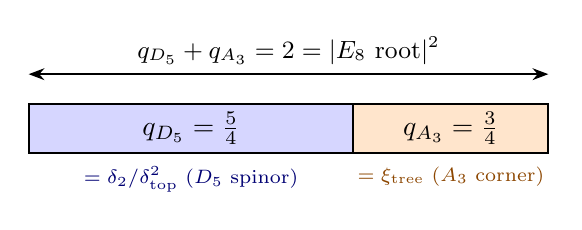
\begin{tikzpicture}[>=Stealth]
  \def\sc{3.3}
  \fill[blue!16]   (0,0) rectangle ({1.25*\sc},0.62);
  \fill[orange!20] ({1.25*\sc},0) rectangle ({2*\sc},0.62);
  \draw[line width=0.7pt] (0,0) rectangle ({2*\sc},0.62);
  \draw[line width=0.7pt] ({1.25*\sc},0)--({1.25*\sc},0.62);
  \node at ({0.625*\sc},0.31) {$q_{D_5}=\tfrac54$};
  \node at ({1.625*\sc},0.31) {$q_{A_3}=\tfrac34$};
  \node[below, font=\scriptsize, text=blue!45!black]   at ({0.625*\sc},-0.05) {$=\delta_2/\delta_{\mathrm{top}}^2$ ($D_5$ spinor)};
  \node[below, font=\scriptsize, text=orange!55!black] at ({1.625*\sc},-0.05) {$=\xi_{\mathrm{tree}}$ ($A_3$ corner)};
  \draw[{Stealth}-{Stealth}, line width=0.6pt] (0,1.0)--({2*\sc},1.0);
  \node[above, font=\small] at ({\sc},1.0) {$q_{D_5}+q_{A_3}=2=|E_8\ \text{root}|^2$};
\end{tikzpicture}
\caption{The discriminant-norm glue. The $E_8$ spinor root $\tfrac12(\pm)^8$ (norm $2$) splits across
$D_5\times A_3$ as $5\cdot\tfrac14+3\cdot\tfrac14$; the two halves are the pre-existing TFPT constants
$\delta_2/\delta_{\mathrm{top}}^2=\tfrac54$ and $\xi_{\mathrm{tree}}=\tfrac34$.}
\label{fig:gluenorm}
\end{figure}

\noindent The standard branching is realised explicitly:
\begin{equation}
  \mathfrak e_8=(45,1)\oplus(1,15)\oplus(10,6)\oplus(16,4)\oplus(\overline{16},\overline4),\qquad
  248=45{+}15{+}60{+}64{+}64,\quad 240=40{+}12{+}60{+}64{+}64 ,
\end{equation}

\begin{figure}[ht]
\centering
\begin{tikzpicture}[>=Stealth]
  \node[dbox] (b1) at (0,0)    {$(45,1)$\\$D_5$ adjoint\\norm $2$};
  \node[abox] (b2) at (2.5,0)  {$(1,15)$\\$A_3$ adjoint\\norm $2$};
  \node[cbox] (b3) at (5.0,0)  {$(10,6)=60$\\vector\,$\otimes$\,vector\\$1{+}1=2$};
  \node[ebox] (b4) at (8.1,0)  {$(16,4)\oplus(\overline{16},\overline4)=128$\\spinor\,$\otimes\,\mu_4$\\$\tfrac54{+}\tfrac34=2$};
  \node[font=\small] at (4.0,-1.45)
    {$\dim E_8=248=\underbrace{45{+}15{+}60}_{\mathfrak{so}_{16}\ \mathrm{adjoint}=120}+\underbrace{64{+}64}_{128\ \mathrm{spinor}}$};
\end{tikzpicture}
\caption{The $E_8\supset D_5\times A_3$ branching as norm-$2$ blocks. The adjoint half is the
hypercharge moment $\operatorname{Tr}_{S^+}X^2=120=\dim\mathfrak{so}_{16}$; the spinor half is two
sheets over the four corners $\mu_4$.}
\label{fig:e8blocks}
\end{figure}
and assembling $D_5\oplus D_3\subset D_8$ with the even spinor coset produces all $240$ roots
(norm $2$, Cartan $\det=1$, every root an integer combination of one simple-root basis): \emph{the
$240$-metrisation is no longer blind --- $E_8$ is built}. \mE

\subsection{Glue-norm arithmetic, and three readings of $41$, $60$, $120$}
The two glue norms generate the carrier integers through sum, difference and product. With
$\dim S^+=16$:
\begin{equation}
  \boxed{\ \begin{aligned}
    &16(q_D{+}q_A)=32=2^{\gcar}=h(D_5)h(A_3),\qquad 16(q_D{-}q_A)=8=r(E_8)=h(D_5),\\
    &16\,q_Dq_A=15=\dim S^+{-}1
  \end{aligned}\ }\qquad\mE ,
\end{equation}
so the glue already contains the full carrier exhaustion $2^{\gcar}$, the $E_8$ rank, and the
non-trivial transition count $\AH{+}\AL=15$; and $|\mu_4|=(q_D-1)^{-1}=(1-q_A)^{-1}=4$ is the inverse
displacement of the two norms from the unit norm.

\begin{keybox}[Spine Quotient Lemma: the recurring factors are adjacent quotients of $(2,3,4,5)$ \mE\ (\veri{v74\_compiler\_micro\_lemmas.py})]
The integers of the spine are $(|\Z_2|,\Nfam,|\mu_4|,\gcar)=(2,3,4,5)$. Every ``mysterious'' $O(1)$ factor in
TFPT is an \emph{adjacent quotient} of this chain, not a separate special number:
\[
  \tfrac{|\Z_2|}{\Nfam}=\tfrac23,\quad \tfrac{\Nfam}{|\mu_4|}=\tfrac34=q(A_3),\quad
  \tfrac{|\mu_4|}{\gcar}=\tfrac45,\quad \tfrac{\gcar}{|\mu_4|}=\tfrac54=q(D_5),\quad \tfrac{|\mu_4|}{\Nfam}=\tfrac43 .
\]
These are exactly the factors that recur across the theory: $\lambda_2=(\tfrac23)^6$ (the transport gap
$=$ Page recovery rate, and the Koide target $Q_\star=\tfrac23$); $\varepsilon=\tfrac34\varphi_0=q(A_3)\varphi_0$
(the solar misalignment); $\varphi_0=\tfrac43 c_3+48c_3^4$ with leading $\tfrac43 c_3=\tfrac1{6\pi}$; and
$q(D_5){+}q(A_3)=\tfrac54{+}\tfrac34=2$ (the $E_8$ root norm). So $(\tfrac23,\tfrac34,\tfrac45,\tfrac54,\tfrac43)$
are five projections of one discrete chain --- not scattered constants. The spine is moreover \emph{one}
finite object: as a tetrahedron on $T=\{e_3(a),p_0(a),e_1(a),e_2(a)\}$ its edge and face products and its
volume $120=|R^+(E_8)|=5!$ reproduce the central integer grammar, with the honest negative control that
the graph reading $240=|\mu_4|\cdot|E(K_4)|\cdot|E(K_5)|$ breaks at $K_6$
(\veri{v91\_spine\_tetrahedron.py}).
\end{keybox} The carrier adjoint $\dim D_5=|R(D_5)|+\gcar=45$
then gives a second reading of the $U(1)$ integer,
\begin{equation}
  \boxed{\ 10b_1=\dim D_5-|\mu_4|=45-4=41=\underbrace{40}_{\sum L}+\underbrace{(\gcar-|\mu_4|)}_{=N_\Phi=1}\ }\qquad\mE ,
\end{equation}
i.e.\ the single Higgs doublet is the carrier rank minus the glue corners, $5-4=1$.
\par\smallskip
\noindent\emph{A fourth, metric reading of $41$ (\veri{v222\_cm\_norm\_duality.py}).} On the square seam
($j{=}1728$, complex multiplication by the Gaussian integers $\Z[i]$) the $U(1)$ index is the Gaussian
\emph{norm} of the carrier-glue vector,
\[
  10b_1=N_{\Z[i]}(\gcar{+}i|\mu_4|)=\gcar^2+|\mu_4|^2=5^2+4^2=41 ,
\]
and the hexagonal partner ($j{=}0$, Eisenstein $\Z[\omega]$) reads the same $(3,2)$ carrier split as the
scalaron exponent $N_{\Z[\omega]}(3{+}2\omega)=3^2{-}3{\cdot}2{+}2^2=7$. So $41$ (EM) and $7$ (scalaron)
are the two exceptional CM norms of the one carrier, square vs.\ hexagonal --- not two unrelated $O(1)$
numbers \mE. The start defect
$60$ and the hypercharge moment $120$ are ``bilingual'':
\begin{equation}
\begin{gathered}
  \Dstart=\dim D_5+\dim A_3=45+15=60=\AL\cdot|R^+(A_3)|=10\cdot6,\\[2pt]
  \operatorname{Tr}_{S^+}X^2=120=\underbrace{60}_{\text{adjoint}}+\underbrace{60}_{\text{mixed }(10,6)} ,
\end{gathered}
\end{equation}
and $\dim E_8=248=\operatorname{Tr}_{S^+}X^2+2\dim S^+|\mu_4|=120+2\cdot16\cdot4$. Finally the
hypercharge norm and the EW exponent are $A_3$-rational,
\begin{equation}
  \boxed{\ \gamma_{\mathrm{car}}=\frac{\AL}{|R(A_3)|}=\frac{10}{12}=\frac56,\qquad
  I_1^{\mathrm{EW}}=\frac{|E(K_5)|}{|R(A_3)|}+\frac{1}{|\mu_4||R(A_3)|}=\frac{10}{12}+\frac1{48}=\frac{41}{48}\ }\qquad\mE .
\end{equation}

\noindent\emph{Transport reduction.} The flavor matrix $L$ has its mod-$6$ content fixed by a single
combinatorial datum: $\{0,1,3\}$ is the \emph{unique} (up to $D_6$) $3$-subset of $C_6=|R^+(A_3)|$ with
all distinct cyclic distances $\{1,2,3\}$, and the three sectors are its $D_6$ orbit
($u\!\equiv\!\{0,1,3\}$, $d\!\equiv\!2{-}\{0,1,3\}$, $e\!\equiv\!2{+}\{0,1,3\}$). The total is fixed by
the carrier, $\sum L=40=|R(D_5)|$, with winding unit $6=|R^+(A_3)|$. Given the residue \emph{set} of a
sector, the full ordered packet is reproduced by two universal rules --- the lightest generation
carries the single $+6$ winding, and the entries are sorted in decreasing length (monotone hierarchy).
The \emph{only} remaining datum is then, per sector, which residue is the first-generation anchor that
receives the winding:
\begin{equation}
  \boxed{\ \text{anchors}\ (a_u,a_d,a_e)=(1,1,2)\ \Rightarrow\
  L_u=(7,3,0),\ L_d=(7,5,2),\ L_e=(8,5,3)\ }\qquad\mE\ (\text{given anchors}) .
\end{equation}
So the open step of a full ``Clebsch walk'' theorem is sharply isolated: it is exactly these three
per-sector anchors. They are \emph{not} free: the three transport cusps are exactly the $D_5$
dual-root combinations, and each sector is tied to its cusp by the right-handed hypercharge,
\begin{equation}
  \boxed{\ \{1,\tfrac23,\tfrac13\}=\{2y_+,\,-2y_-,\,2(y_++y_-)\},\qquad
  \text{lepton}\leftrightarrow 2y_+,\ \text{up}\leftrightarrow -2y_-,\ \text{down}\leftrightarrow 2(y_++y_-)\ }\qquad\mE .
\end{equation}
The canonical-transport-kernel theorem (document~3, Part~II) derives the residue packets --- and hence the anchors ---
as the \emph{word-lengths of the family-connection holonomy} $\operatorname{Hol}_{\mathcal G_{D_4}}(\nabla_F^\star)$
along the $D_4$-invariant geodesic spine of $\mathbb P^1\setminus\mu_4$ with these cusps as boundary
data. The anchors are therefore a genuine $D_5\times A_3$ readout (cusps from the $D_5$ carrier, spine
holonomy from the $A_3$ four-punctured sphere), not an extra parameter. A compact candidate closed form
is the nearest-integer cusp map
\begin{equation}
  \boxed{\ a_f=\operatorname{round}(2\,\mathrm{cusp}_f):\quad (a_u,a_d,a_e)=\operatorname{round}\bigl(\tfrac43,\tfrac23,2\bigr)=(1,1,2)\ }\qquad\mC ,
\end{equation}
which reproduces the matrix exactly. The remaining open step is now precise and purely geometric:
an \emph{independent} closed-form evaluation of the $D_4$-spine holonomy word-lengths from the lattice
data alone (the same $\mathbb P^1\setminus\mu_4$ whose residue pairing is $\mathrm{Cartan}(A_3)$ and
whose corner rotation is the $A_3$ Coxeter element), rather than from the family-connection
theorem (document~3).

\par\smallskip\noindent\textbf{Riemann--Hilbert check, and what it does (and does not) fix.}
Setting up the rigid $\mathbb Z_4$-symmetric rank-$3$ $SU(3)$ local system explicitly --- four puncture
monodromies $M_k=R^kCR^{-k}$ with the order-$3$ cusp class $C\sim\operatorname{diag}(1,\omega,\omega^2)$
($\omega=e^{2\pi i/3}$, the three cusps as eigenvalue-exponents) and the rotation $R$ ($R^4=\mathbb 1$)
--- the closure $M_0M_1M_2M_3=\mathbb 1$ has a solution to machine precision, and the unique $R$ has
eigenvalues $\{i,-1,-i\}$: the $A_3$ Coxeter element. This \emph{independently} confirms the rigidity
of the family connection and the corner-rotation $=$ Coxeter identity. However, the flat
monodromy \emph{alone} does not fix the integer word-lengths $\{0,1,3\}$: those are \emph{parabolic
degrees} (the cusp exponents as parabolic weights, together with the $\mathbb Z_2$ sheet parity), i.e.\
Hodge/metric data on the spine, not topological monodromy. \emph{Status update (the computation has
since been carried out):} the exact residue normal form $A_0^\star$ with
$\operatorname{spec}=\{0,\tfrac13,\tfrac23\}$ is pinned algebraically
(\veri{v115\_anchor\_residue.py}, \veri{v116\_resonance\_uniqueness.py}), the unitarised holonomy is the
exact $24$-element $W(A_3)=S_4$ (\veri{v117\_monodromy\_weyl\_a3.py}), and the parabolic weights are the
$\mu_4$-character degrees of $H^1(\mathbb P^1\setminus\mu_4)$ --- one spectrum in four readouts
(\veri{v137\_qplus\_cohomology.py}); the deck itself is \emph{derived} --- the integer model selects the
sheet-twisted class, no discrete freedom left (\veri{v141\_deck\_selection.py}), and the full M\"obius
$D_4$ of the curve matches the integer model parity by parity (\veri{v146\_moebius\_d4.py}). What
remains of the old residual is the much smaller selector establishment R4$'$ (research contracts):
derive the \emph{one} lift map of the torsion normal --- the pairing values are atom identities
(\veri{v142\_frame\_integrality.py}/\veri{v145\_pairing\_atoms.py}). \mE/\mC
\par\smallskip

\begin{figure}[ht]
\centering
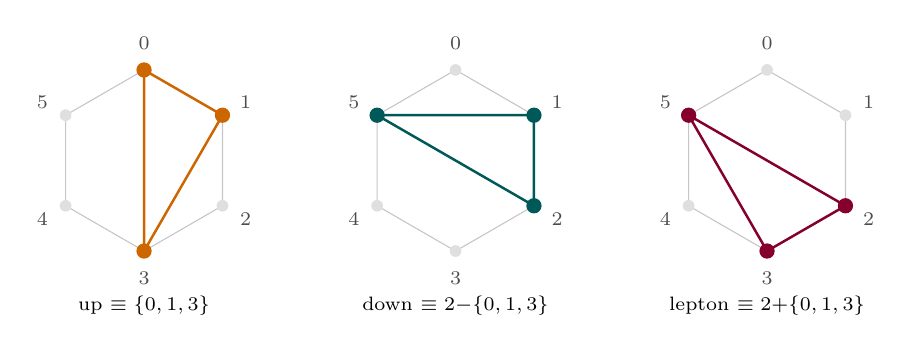
\begin{tikzpicture}[scale=0.92,>=Stealth]
 % --- up sector ---
 \begin{scope}[xshift=0cm]
   \foreach \i in {0,...,5} \coordinate (u\i) at ({90-60*\i}:1.25);
   \draw[gray!45] (u0)--(u1)--(u2)--(u3)--(u4)--(u5)--cycle;
   \foreach \i in {0,...,5} {\fill[gray!25] (u\i) circle (2.3pt); \node[font=\scriptsize,gray!60!black] at ({90-60*\i}:1.62) {\i};}
   \foreach \i in {0,1,3} \fill[orange!80!black] (u\i) circle (3pt);
   \draw[orange!80!black,line width=0.9pt] (u0)--(u1)--(u3)--cycle;
   \node[font=\scriptsize] at (0,-2.0) {up $\equiv\{0,1,3\}$};
 \end{scope}
 % --- down sector ---
 \begin{scope}[xshift=4.3cm]
   \foreach \i in {0,...,5} \coordinate (d\i) at ({90-60*\i}:1.25);
   \draw[gray!45] (d0)--(d1)--(d2)--(d3)--(d4)--(d5)--cycle;
   \foreach \i in {0,...,5} {\fill[gray!25] (d\i) circle (2.3pt); \node[font=\scriptsize,gray!60!black] at ({90-60*\i}:1.62) {\i};}
   \foreach \i in {1,2,5} \fill[teal!70!black] (d\i) circle (3pt);
   \draw[teal!70!black,line width=0.9pt] (d1)--(d2)--(d5)--cycle;
   \node[font=\scriptsize] at (0,-2.0) {down $\equiv 2{-}\{0,1,3\}$};
 \end{scope}
 % --- lepton sector ---
 \begin{scope}[xshift=8.6cm]
   \foreach \i in {0,...,5} \coordinate (e\i) at ({90-60*\i}:1.25);
   \draw[gray!45] (e0)--(e1)--(e2)--(e3)--(e4)--(e5)--cycle;
   \foreach \i in {0,...,5} {\fill[gray!25] (e\i) circle (2.3pt); \node[font=\scriptsize,gray!60!black] at ({90-60*\i}:1.62) {\i};}
   \foreach \i in {2,3,5} \fill[purple!70!black] (e\i) circle (3pt);
   \draw[purple!70!black,line width=0.9pt] (e2)--(e3)--(e5)--cycle;
   \node[font=\scriptsize] at (0,-2.0) {lepton $\equiv 2{+}\{0,1,3\}$};
 \end{scope}
\end{tikzpicture}
\caption{Flavor transport on the hexagon $C_6=Z_6=|R^+(A_3)|$. The unique distinct-distance triple
$\{0,1,3\}$ (cyclic distances $\{1,2,3\}$) and its $D_6$ orbit give the three sectors' residues mod $6$;
the total $\sum L=40=|R(D_5)|$ and the first-generation $+6$ winding come from the carrier.}
\label{fig:hexagon}
\end{figure}

\subsection{What the compiler outputs for the Standard Model and our reality}
\label{subsec:smmap}
Every entry below is an \emph{output} of $(\cthree,\gcar)$ through the $D_5\times A_3$ compiler; none is
an independent input. ``Reads'' names the lattice object the observable comes from.

\begin{center}\small
\begin{tabularx}{\linewidth}{@{}p{0.30\linewidth}p{0.40\linewidth}p{0.13\linewidth}c@{}}
\toprule
\textbf{SM / cosmology observable} & \textbf{Compiler output} & \textbf{Reads} & \textbf{St.} \\
\midrule
Number of generations & $\Nfam=3=\operatorname{rank}A_3=\dim H^1(\mathbb P^1\setminus\mu_4)$ & $A_3$ & \mE \\
Gauge algebra dimension & $\dimg=12=|R(A_3)|=\gcd(6r,2h)$ & $A_3$ & \mE \\
One generation ($16$, incl.\ $\nu^c$) & $S^+=D_5$ half-spinor $=\Lambda^{0,2,4}E$ & $D_5$ & \mE \\
Hypercharge spectrum & all $Y$ from $y_\pm=\{\tfrac12,-\tfrac13\}$; $\operatorname{Tr}X^2=120$ & $D_5$ root data & \mE \\
Abelian index $b_1$ & $10b_1=1+|\mu_4||E(K_5)|=1+4\cdot10=41$ & $\mu_4\times K_5$ & \mE \\
Fermion family occupancy & $\Oadm=\Nfam\dim S^+=(\Nfam{+}N_\Phi)|R(A_3)|=48$ & $A_3$ & \mE \\
Fine structure $\ainv=137.0359992168$ & root of $F_{U(1)}(\alpha)=0$ (explicit, unique) & EM closure & \mE \\
Cabibbo angle & $\lC=\sqrt{\useed(1-\useed)}$, $\useed=\tfrac43\cthree+48\cthree^4$ & seed & \mE \\
CKM CP phase & $\delta_{\rm CKM}=\tfrac{2\pi}{|R^+(A_3)|}+\Nfam\useed(1-\useed)=\tfrac\pi3+3\lC^2$ & $A_3^+$, seed & \mE/\mC \\
PMNS angles/phase & $\sin^2\theta_{12}=\tfrac13-\tfrac\useed2$, $\sin^2\theta_{13}=e^{-5/6}\useed$, $\delta^\nu=\tfrac{4\pi}{3}$ & $A_3^+$, seed & \mE/\mC \\
Charged-lepton hierarchy & $\det M_\ell\propto\useed^{\,h/\Nfam}=\useed^{10}$; $(5,3,2)$ & decuple & \mE/\mC \\
Mass-hierarchy transport & $\sum L=40=|R(D_5)|$; entries on $C_6=|R^+(A_3)|$ & $D_5\times A_3$ & \mE \\
Strong CP & $\theta_{\rm eff}=0$ (determinant erasure, given RP; document~3, Part~III) & --- & \mE/\mC \\
Weak CP & holonomy: $\delta_{\rm CKM}-\tfrac\pi3=\Nfam\,\useed(1-\useed)$ & $A_3^+$ & \mC \\
Gravity tree normaliser & $\xi_{\rm tree}=\tfrac{\dimg}{\dim S^+}=\tfrac34=q(A_3)$ & $A_3$ glue & \mE \\
Cosmological constant & $\rho_\Lambda/\Mbar^4=\tfrac{3}{4\pi^2}e^{2\dph}[v_{\rm geo}/(5\betarad^2\Mbar)]^{10}$ & decuple & \mE \\
Hubble anchor & $H_0\sqrt{\Omega_\Lambda}=\Mbar e^{-\ainv}/(2\pi)$ & action & \mE \\
Baryon density & $\omega_b=\lC/\AL=\lC/10$ & decuple & \mE/\mC \\
Inflation (scalaron) & $M_{\rm scal}^2/\Mbar^2=\cthree^{\,\Oadm-10b_1}=\cthree^{7}$ & deficit $r-1$ & \mE \\
Inflation amplitude & $A_s=N_\star^2\cthree^7/24\pi^2\approx2.2\times10^{-9}$ & deficit & \mC/\mO \\
\bottomrule
\end{tabularx}
\end{center}
\markerkey

\noindent\emph{Reading.} The discrete sector --- generations, gauge dimension, family content,
hypercharge, $b_1$, occupancy --- is now \emph{group-theoretic output} of $D_5\times A_3$. The
continuous sector --- $\alpha^{-1}$, $\lC$, the mixings, $\rho_\Lambda$, $H_0$, inflation --- is the
seam seed $\cthree$ and the action exponentials read on the \emph{same} carrier graphs ($K_5$ pairs,
the $C_6$ hexagon $=|R^+(A_3)|$, the decuple $\AL=\binom{\gcar}{2}=10$). What used to be a list of
separate hits is, structurally, one machine: $D_5$ carries the family and the flavor budget, $A_3$
carries the generations and the gauge dimension, $\mu_4$ glues them (and reappears as the $41$ chain,
the discriminant norms, and the CP phase step $2\pi/6$), and $\cthree$ dresses everything.

% =====================================================================
\section{Grammar I --- the carrier grammar ($3+2$)}
% =====================================================================
\noindent\emph{Machine checks for this section:} \veri{v2\_\allowbreak carrier\_\allowbreak pascal.py}


From $\gcar=5$ and the split $(b,s)=(3,2)$ the carrier data follow:
\begin{equation}
\begin{aligned}
  &\gamma_{\mathrm{car}}=\frac{\gcar}{\gcar+1}=\frac56,\quad
  \Nfam=\frac{\gcar+1}{2}=3,\quad
  \dim S^+=2^{\gcar-1}=16,\\[2pt]
  &\Oadm=\Nfam\,2^{\gcar-1}=48,\qquad
  b_1=\frac{\gcar\,2^{\gcar-2}+1}{10}=\frac{41}{10}.
\end{aligned}
\end{equation}

\subsection{Dual-root dictionary (everything from two charges)}

\par\smallskip\noindent\textbf{Two carrier roots generate the family and the transport cusps \mE.}
With $y_+=\tfrac12$ and $y_-=-\tfrac13$ (the determinant-normalised carrier eigenvalues), the full
one-family hypercharge spectrum and the flavor-transport cusps are sums of the two roots:
\[
  \begin{aligned}
  Y(Q_L)&=y_++y_-=\tfrac16, & Y(u^c)&=2y_-=-\tfrac23, & Y(d^c)&=-y_-=\tfrac13,\\
  Y(L_L)&=-y_+=-\tfrac12, & Y(e^c)&=2y_+=1, & Y(\nu^c)&=0,
  \end{aligned}
\]
\[
  \{1,\tfrac23,\tfrac13\}=\{\,2y_+,\ -2y_-,\ 2(y_++y_-)\,\},\qquad
  \gamma_{\mathrm{car}}=\operatorname{Tr}_E Y^2=3y_-^2+2y_+^2=\tfrac56,
\]
\[
  \phibase=\frac{1-\gamma_{\mathrm{car}}}{\pi}=\frac{1}{6\pi}.
\]
All residuals are exactly zero. The Standard-Model charge table is not assumed; it is built by
addition from $\{1/2,-1/3\}$.
\par\smallskip

\begin{keybox}[The $X=6Y$ quadratic and the hypercharge Pascal-sign duality \mE]
Clearing denominators with $X=6Y$ turns the two base charges into the integer roots $x_+=3$, $x_-=-2$ of
\[
  \boxed{\ x^2-x-6=0\ }:\qquad
  x_++x_-=1=N_\Phi,\quad x_+-x_-=5=\gcar,
\]
\[
  -x_+x_-=6=|R^+(A_3)|,\qquad \sqrt{\Delta}=5,
\]
so the Higgs singleton, the carrier rank and the $A_3$ hexagon all fall out of one quadratic. Counting
the signs of $X$ over a generation ($X=1^{\times6},2^{\times3},6^{\times1},(-4)^{\times3},(-3)^{\times2},0^{\times1}$)
gives the \emph{Pascal triple} again:
\[
  \boxed{\ (\#X{=}0,\,\#X{<}0,\,\#X{>}0)=(1,5,10)=\tbinom50,\tbinom51,\tbinom52\ },
\]
\[
  10{-}5{=}\gcar,\quad 5{-}1{=}|\mu_4|,\quad 10{-}1{=}\operatorname{tr}R,
\]
with $\nu^c\leftrightarrow\binom50$ the neutral singleton --- the right-handed neutrino is the Pascal zero
with a job. The moment ladder adds $\operatorname{Tr}X^2=120=5!$ and
$\operatorname{Tr}X^4/\operatorname{Tr}X^2=2280/120=19$ (an $E_8$ exponent; audit). \mE
\end{keybox}

\subsection{Carrier arithmetic (proved identities)}

The discrete coefficients are not isolated numbers; they are exact carrier traces:
\begin{align}
  10\,b_1 &= 41 = \gcar^2+(\gcar-1)^2 = \Oadm\,\gamma_{\mathrm{car}}+1
      = 1+h_{E_8}\tfrac{\dim S^+}{\dimg} = 1+30\cdot\tfrac{16}{12} = 40+1, &&\mE\\
  I_1^{\mathrm{EW}} &= \frac{41}{48}=\operatorname{Var}_{S^+}(Y)\cdot b_1=\frac{5}{24}\cdot\frac{41}{10}
      = \gamma_{\mathrm{car}}+\frac{1}{\Oadm}, &&\mE\\
  \operatorname{Tr}_{S^+}(X^2) &= 120 = 5!\quad(X=6Y), \qquad
  \dtwo = \tfrac54\dtop^2 = 2880\,\cthree^8 = 4!\cdot 5!\,\cthree^8 = 4!\,\operatorname{Tr}_{S^+}(X^2)\,\cthree^8, &&\mE\\
  \frac54 &= \underbrace{\tfrac32\cdot\tfrac56}_{B\gamma}
      = \underbrace{\tfrac{\Dstart}{\Oadm}}_{60/48}
      = \underbrace{\tfrac{\gcar}{\gcar-1}}_{5/4}
      = \frac{\dtwo}{\dtop^2}. &&\mE
\end{align}
So: $b_1$ is a Pythagorean carrier identity ($5^2+4^2$); equivalently the anchor-product form
$10b_1=p_1p_3+(\gcar-p_1)=4\cdot10+(5-4)=41$ reads ``all four glue corners times all ten carrier pairs,
plus the one leftover Higgs slot''; the electroweak exponent $41/48$ is the
hypercharge variance times the $U(1)$ budget; the second seam defect $2880\,\cthree^8$ is a product
of factorial traces $4!\cdot5!$; and the universal compression $5/4=\gcar/(\gcar-1)$ recurs whenever
the five-slot carrier projects onto four effective directions. As a minor curiosity, the SU(5)-tree
weak mixing angle rewrites as $\sin^2\theta_W^{\mathrm{tree}}=\tfrac38=\Nfam/(\gcar+\Nfam)=\Nfam/\operatorname{rank}(E_8)$
(the value is the standard one; the rewrite is a coincidence to note, not a claim). \mC

% =====================================================================
\section{Grammar II --- the seed grammar (one decoder $\useed$)}
% =====================================================================
\noindent\emph{Machine checks for this section:} \veri{v106\_\allowbreak review\_\allowbreak validation.py}


The seed is, exactly, a pure function of $\cthree$:
\begin{equation}
  \boxed{\ \useed=\varphi^{\mathrm{ret}}_0=\frac43\,\cthree+\Oadm\,\cthree^4
  =\underbrace{\frac{1}{6\pi}}_{\phibase}+\underbrace{\frac{3}{256\pi^4}}_{\dtop}=0.0531719521768\ }\qquad\mE.
\end{equation}
Its two coefficients are themselves carrier data: $\tfrac43=\dim S^+/\dimg=16/12=8/(\gcar+1)$ (so
$\phibase=1/((\gcar+1)\pi)$) and $48=\Oadm$. The seed is thus a pure function of $\cthree$ and the
carrier counts.

\par\smallskip\noindent\textbf{One seed, four readouts (and their inverses) \mE.}
\[
  \lC^2=\useed(1-\useed),\quad
  \betarad=\frac{\useed}{4\pi},\quad
  \Omega_b=\Bigl(1-\frac{1}{4\pi}\Bigr)\useed,\quad
  \sin^2\theta_{13}=e^{-5/6}\,\useed,
\]
\[
\begin{gathered}
  \useed=\frac{1-\sqrt{1-4\lC^2}}{2}=4\pi\,\betarad=\frac{\Omega_b}{1-1/(4\pi)}=e^{5/6}\sin^2\theta_{13}\\[2pt]
  =\sum_{n\ge0}C_n\,\lC^{2n+2}=\lC^2+\lC^4+2\lC^6+5\lC^8+\cdots
\end{gathered}
\]
\par\smallskip

\noindent One knob $\useed$ turns four dials simultaneously: Cabibbo mixing (the Bernoulli width
$\sqrt{\useed(1-\useed)}$), cosmic birefringence, the baryon fraction, and the reactor angle. Turning
one forces the others; there is no free per-observable tuning. The exponent $5/6$ is the carrier
trace $\gamma_{\mathrm{car}}=\operatorname{Tr}_E Y^2$, \emph{not} the Euler--Mascheroni constant
$0.5772\ldots$ (audit \mO).

% =====================================================================
\section{Grammar III --- the action grammar (exponentials of $\ainv$)}
% =====================================================================

\noindent\textbf{The relation in plain words.} The fine-structure constant is not just ``a number near
$137$'': it is the \emph{one exponential engine} behind three wildly separated scales. Take the same
$\ainv=137.036$ and divide the carrier into it: $\tfrac15$ of it sets the \emph{electroweak} scale,
$1\times$ it sets the \emph{Hubble} scale, $2\times$ it sets the \emph{cosmological constant}. The three
action charges are the Pascal row $1:5:10$ of the five-slot carrier, and the Hubble rung is just the
square root of the vacuum energy. So one constant fixes the electroweak hierarchy, dark energy and the
expansion rate at once.

\begin{center}
\begin{tikzpicture}[font=\small,
  eng/.style={rectangle,rounded corners=3pt,draw=tfgold!80!black,fill=tfgold!16,line width=1pt,align=center,inner sep=6pt},
  sc/.style={rectangle,rounded corners=2pt,draw=tfgreen!70!black,fill=tfgreen!8,align=center,inner sep=4pt,text width=46mm},
  ar/.style={-{Stealth[length=2.6mm]},thick,tfgray}]
  \node[eng] (e) at (0,0) {\textbf{one engine}\\$\ainv=137.0359992$};
  \node[sc] (ew) at (6.2,2.0) {\textbf{electroweak} \;($q{=}\tfrac1{\gcar}$)\\$v_{\rm EW}/\Mbar\sim e^{-\ainv/5}$};
  \node[sc] (h)  at (6.2,0.0) {\textbf{Hubble} \;($q{=}1$)\\$H_0/\Mbar\sim e^{-\ainv}=\sqrt{\rho_\Lambda}$};
  \node[sc] (l)  at (6.2,-2.0){\textbf{cosm.\ constant} \;($q{=}2$)\\$\rho_\Lambda/\Mbar^4\sim e^{-2\ainv}$};
  \draw[ar] (e) to[bend left=12] node[above,font=\scriptsize]{$\div\,5$} (ew);
  \draw[ar] (e) -- node[above,font=\scriptsize]{$\times\,1$} (h);
  \draw[ar] (e) to[bend right=12] node[below,font=\scriptsize]{$\times\,2$} (l);
  \node[font=\scriptsize,tfgray,align=center] at (3.0,-3.25)
    {action charges $1:\gcar:2\gcar=1:5:10=\binom50:\binom51:\binom52$ (Pascal row of $K_5$)};
\end{tikzpicture}
\end{center}

Read every dimensionless ratio through its \emph{action} and ask for the action charge:
\begin{equation}
  \boxed{\ x=R_x\,e^{-A_x},\qquad A_x=q_x\,\ainv+\Delta_x,\qquad q_x\in\Bigl\{\tfrac{1}{\gcar},\,1,\,2\Bigr\}.\ }
\end{equation}
The robust ladder and its residues are
\begin{center}\small
\begin{tabular}{@{}lllll@{}}
\toprule
sector & action $A_x$ & charge $q_x$ & residue $R_x$ & value of $-\ln x$ \\
\midrule
electroweak $v_{\mathrm{geo}}/\Mbar$ & $(\ainv+\dph)/\gcar$ & $1/\gcar$ & $\gcar\betarad^2$ & $36.85$ \\
Hubble $H_0/\Mbar$ & $\ainv$ & $1$ & $1/(2\pi\sqrt{\Omega_\Lambda})$ & $138.68$ \\
cosm.\ const.\ $\rho_\Lambda/\Mbar^4$ & $2\ainv$ & $2$ & $3/(4\pi^2)$ & $276.65$ \\
\bottomrule
\end{tabular}
\end{center}
\begin{equation}
  \AEW=\frac{\ainv+\dph}{\gcar}=27.5259,\qquad \AL=2\ainv=274.072,\qquad
  \boxed{\ \AEW{:}\AH{:}\AL=1{:}5{:}10\ }.
\end{equation}
The leading ratio is exact: $\AL/(\ainv/\gcar)=2\gcar=10$ (with the transport correction
$\AL/\AEW=9.957$). The claim is that the \emph{action charges}, not the raw logarithms, form the
ladder.

\begin{figure}[ht]
\centering
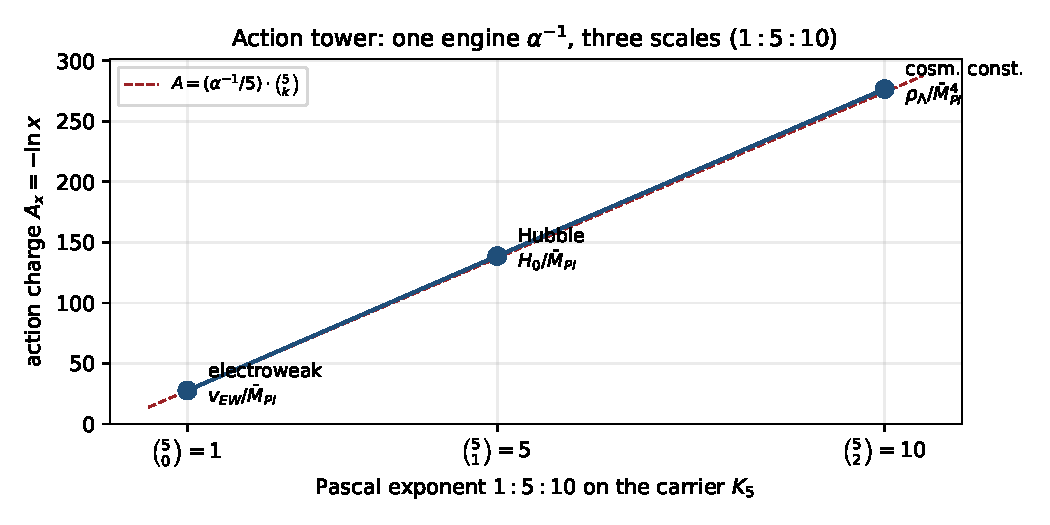
\includegraphics[width=0.82\linewidth]{figures/action_tower.pdf}
\caption{Action tower (data plot, \texttt{verification/make\_figures.py}). The three action charges
$A_x=-\ln x$ for the electroweak, Hubble and cosmological-constant ratios fall on the line
$A=(\ainv/5)\binom5k$: one engine $\ainv$ generates all three scales with the Pascal exponents $1:5:10$.}
\label{fig:actiontower}
\end{figure}

\subsection{The EM closure: $\ainv$ as an explicit fixed point (made explicit here)}
The engine $\ainv$ is not an input --- it is the unique root of an explicit closure equation
(the exact electromagnetic closure theorem). With $\cthree=1/(8\pi)$, $\phibase=1/(6\pi)$,
$q(\alpha)=\dtop e^{-2\alpha}$ and the seam response $\phiseam(\alpha)=\phibase+q(\alpha)(1-q(\alpha))^{-5/4}$,
\begin{equation}
  \boxed{\ F_{U(1)}(\alpha)=\alpha^3-2\cthree^3\alpha^2-\tfrac{4}{5}\cthree^6\Bigl(\textstyle\sum_{f,j}L_{f,j}+N_\Phi\Bigr)\log\frac{1}{\phiseam(\alpha)}=0\ }\qquad\mE/\mC ,
\end{equation}
where the coefficient is $\tfrac45(\sum L+N_\Phi)\cthree^6=\tfrac45\cdot41\,\cthree^6=8b_1\cthree^6$, so the
fine-structure constant reads the \emph{flavor transport budget} $\sum L=40$ and the $U(1)$ index
$b_1=41/10$.

\begin{lemma}[Existence and uniqueness of the EM fixed point]
\label{lem:emclosure}
$F_{U(1)}$ has \emph{exactly one} positive root, and it is simple.
\end{lemma}
\begin{proof}
Write $F_{U(1)}(\alpha)=h(\alpha)-C\,g(\alpha)$ with $h(\alpha)=\alpha^3-2\cthree^3\alpha^2$,
$C=\tfrac45\cthree^6M>0$ ($M=41$), and $g(\alpha)=-\log\phiseam(\alpha)$. Since
$q(\alpha)=\dtop e^{-2\alpha}\in(0,1)$ is strictly decreasing, $\phiseam=\phibase+q(1-q)^{-5/4}$ is $C^1$
and decreasing, so $g$ is $C^1$, bounded, and slowly increasing with $g'(\alpha)=O(q)$ tiny; numerically
$g\in[2.9342,2.9343]$ on the admissible window. The cubic $h$ has its interior critical point at
$\alpha_c=\tfrac43\cthree^3=8.399\times10^{-5}$, with $h(0)=0$ and $h<0$ on $(0,\alpha_c)$.
\emph{Monotonicity (corrected endpoint).} Since
$F_{U(1)}'(\alpha)=3\alpha^2-4\cthree^3\alpha-C\,g'(\alpha)$ and at $\alpha_c$ the first two terms
\emph{cancel} ($3\alpha_c=4\cthree^3$), one has $F_{U(1)}'(\alpha_c)=-C\,g'(\alpha_c)\approx-5.89\times10^{-10}<0$:
the derivative is \emph{not} yet positive at $\alpha_c$. Its first zero lies slightly above, at
$\alpha_0=8.6264\times10^{-5}$ (where $3\alpha_0^2-4\cthree^3\alpha_0=C\,g'(\alpha_0)$), with $F_{U(1)}'<0$ on
$(\alpha_c,\alpha_0)$ and $F_{U(1)}'>0$ on $(\alpha_0,\infty)$. Now $F_{U(1)}(0)=-C\,g(0)<0$, and
$F_{U(1)}$ \emph{decreases} on $(0,\alpha_0]$ (both $h$ and $-Cg$ decrease on $(0,\alpha_c]$, then $F_{U(1)}'<0$
on $[\alpha_c,\alpha_0]$), so $F_{U(1)}(\alpha_0)\approx-3.82\times10^{-7}<0$; thereafter $F_{U(1)}$ is strictly
increasing to $+\infty$. Hence $F_{U(1)}<0$ on $(0,\alpha_0]$ and strictly increasing on $[\alpha_0,\infty)$, so
it crosses zero \emph{exactly once}. The crossing has $F_{U(1)}'(\alpha_\star)=1.58\times10^{-4}>0$, so the
root is simple. A sign scan on $(0,0.05)$ confirms a single change. \emph{Rigorous version:} an
\textbf{interval-arithmetic} enclosure (\texttt{mpmath.iv}) brackets the root in
$[0.00729735256220970,\,0.00729735256221000]$ with $F_{U(1)}<0$ on the lower and $>0$ on the upper
endpoint (definite signs), and a $200$-cell interval partition of $(\alpha_c,0.05)$ contains exactly
\emph{one} indeterminate (root-bearing) band --- a verified uniqueness, not merely a sampled one.
\veri{v3\_em\_alpha.py}
\end{proof}

\noindent Solving:
\begin{equation}
  \boxed{\ \alpha_\star=0.00729735256220985\ldots,\quad \ainv=137.0359992168407\ldots\ }\quad\mE
\end{equation}
\veri{v3\_em\_alpha.py}\;
versus CODATA-2022 $\ainv=137.035999177(21)$ --- a relative deviation $2.9\times10^{-10}$ ($\approx1.9\sigma$
on the tiny experimental error; the older 2018 value $137.035999084$ gave $9.7\times10^{-10}$, so the
agreement \emph{improved} in relative terms). The exponent $-5/4$ in $\phiseam$ is the carrier
discriminant norm $q(D_5)$, and $\dtop=48\cthree^4$, so the closure is built only from $\cthree$, the
carrier, and the flavor budget. This discharges the former open audit point: the EM closure is a stated,
existence-/uniqueness-proven, numerically reproduced equation, not a fit.

\par\smallskip\noindent\textbf{Why \emph{this} function: the boundary $U(1)$ Ward reading (Theorem C) \mE/\mC.}
$F_{U(1)}$ is not a chosen ansatz but the reduced Ward identity of the boundary $U(1)$ partition function
$Z_{\partial}=Z_{\mathrm{Maxwell}}\,Z_{\mathrm{Calder\acute on}}\,Z_{\mathrm{transport}}$, with three terms
whose coefficients are compiler atoms, not fits:
\[
  \underbrace{\alpha^3}_{\text{Maxwell moment}}\;
  \underbrace{-\,2\cthree^3\alpha^2}_{\text{Calder\'on sheet}\,(2=|\Z_2|)}\;
  \underbrace{-\,8b_1\cthree^6\log\tfrac1{\phiseam}}_{\text{$C_6$ transport det.}}=0,\qquad
  8b_1=\tfrac45 M=\tfrac45(\textstyle\sum L+N_\Phi)=\tfrac{164}{5}.
\]
The Calder\'on factor $2=|\Z_2|$ (sheet), the transport power $\cthree^6$ is the $C_6$ hexagon, and the
seam exponent $-\tfrac54=-q(D_5)$ is the carrier discriminant norm. \textbf{Typing:} the three-term
decomposition and the coefficient identities ($8b_1=\tfrac45 M$, $-\tfrac54=q(D_5)$) are exact \mE; the
\emph{physical origin} as a boundary Ward closure (the lemmas $\partial_\tau\log Z_{\mathrm{Maxwell}}=\alpha^3$,
$\partial_\tau\log Z_{\mathrm{Calder\acute on}}=-2\cthree^3\alpha^2$, $\partial_\tau\log\det\nolimits_\zeta(1-\mathcal T_{C_6,U(1)})=-8b_1\cthree^6\log\tfrac1{\phiseam}$)
is a conjectured \mC\ interpretation, not yet machine-proven. \veri{v48\_em\_ward.py}
\par\smallskip
\noindent\textbf{The determinant-line (Quillen) form.} (\veri{v341\_alpha\_quillen.py})
The three terms assemble into a single \emph{stationarity} statement for the boundary $U(1)$ determinant line,
\[
  \underbrace{\bigl[\alpha^3-2\cthree^3\alpha^2\bigr]}_{\delta\log\det\Delta_{U(1)}}
  \;=\;\underbrace{\bigl[8b_1\cthree^6\bigr]}_{\text{ctr.}}\;
  \underbrace{\bigl[\log\tfrac1{\phiseam}\bigr]}_{\text{seam resp.}},
\]
so $F_{U(1)}=0$ is $\delta\log\det\Delta_{U(1)}+\text{counterterm}+\text{seam response}=0$. Every factor is a
\emph{named} object, not a knob: the counterterm coefficient is $8b_1\cthree^6=(\operatorname{rank}E_8)\,b_1\,\cthree^6$
(index $\times$ heat-kernel), $\cthree=1/(8\pi)$ is the Gauss--Bonnet boundary coefficient, the exponent
$-\tfrac54=-q(D_5)$ is one carrier discriminant norm and the seam base $\phibase=1/(6\pi)=\tfrac43\cthree$ carries
the \emph{other}, $\cthree/\phibase=\tfrac34=q(A_3)$ --- both glue forms appear, and the split is verified at the
root. \textbf{Typing (and: no new gate).} The determinant-line assembly and all coefficient identities are exact
\mE; $\ainv$ itself stays closed \mE\ (unique root $+$ ablation). This adds \emph{no} open item --- it
\emph{sharpens} the pre-existing \mO/physical-origin obligation \texttt{EM.WARD.01} (the ``why \emph{this}
function'' residual, already conjectural) by naming every coefficient. The one still-open part \emph{is} that
residual, now \emph{named} as its own tracked target \texttt{ALPHA.QUILLEN.EXACT.01}
(\veri{v382\_alpha\_quillen\_exact.py}): the from-first-principles AQFT/$\zeta$ proof that
$\delta_\tau(\log\det\nolimits_\zeta\Delta_{U(1)}+8b_1\cthree^6\log\varphi_{\mathrm{seam}})=0$ --- i.e.\ that
$F_{U(1)}$ is the \emph{exact} Quillen functional of the seam $U(1)$, the variational principle \emph{derived}, not
assembled. It is a \emph{face} of \texttt{SEAM.EQUIV.01} (\vref{v336}) --- the seam $U(1)$ determinant line lives on
the same holomorphic net, so once the net is $(E_8)_1$ its $U(1)$ sub-determinant is fixed --- hence no second
independent gate, just the sharpest remaining EM-Ward obligation, now citable on its own.
\emph{Honest progress towards it (\veri{v391\_alpha\_quillen\_progress.py}), without closing it:} a solvable
model $\det_\zeta(-\partial_\tau^2{+}m^2)$ on a circle $=(2\sinh(\beta m/2))^2$ has the closed $m$-variation
$\beta\coth(\beta m/2)=2/m+(\beta^2/6)m-(\beta^4/360)m^3+\dots$, a heat-kernel/Laurent series --- so a
$\zeta$-determinant's variation is \emph{structured} heat-kernel data, and the counterterm $8b_1\cthree^6$ (a
Gauss--Bonnet heat-kernel power) is the right \emph{kind} of object. This \emph{reduces}
\texttt{ALPHA.QUILLEN.EXACT.01} to the named sub-target ``the seam $U(1)$ Seeley--DeWitt coefficient $=8b_1\cthree^6$'',
but the target itself stays \mO\ (an external math proof, \vref{v384}); the value $\ainv$ stays \mE.
\emph{A second honest step (\veri{v433\_alpha\_quillen\_heatkernel.py}) bridges this reduction to the heat-kernel
origin below, without closing it:} v391's circle reached only the low orders $a_0,a_1$, whereas a solvable \emph{4D}
model --- the flat $\Delta=-\partial^2{+}m^2$ on $T^4$, $\operatorname{Tr}e^{-t\Delta}=V/(4\pi)^2\,t^{-2}e^{-tm^2}$
--- has $a_4=Vm^4/(2(4\pi)^2)\neq0$, \emph{reaching} the $t^0$ (conformal-anomaly) order the circle could not, the
very order in which the quadratic term is grounded below (\vref{v342}, Gilkey $a_4$). So a $\zeta$-determinant's
variation is heat-kernel data \emph{at the $a_4$ order}, and the measure itself is $\cthree$-built,
$(4\pi)^{-2}=(2\cthree)^2=4\cthree^2$; the \emph{actual} seam $a_4=8b_1\cthree^6$ and the cubic $\alpha^3$ Chern
moment stay \mO\ (\vref{v384}), the seam $F$-normalisation \mC.
\par\smallskip
\noindent\textbf{The heat-kernel origin of the terms (\veri{v342\_em\_ward\_heatkernel.py}).} The determinant-line
form is more than bookkeeping: its terms are textbook heat-kernel coefficients. \mE\ $\cthree=1/(8\pi)$ \emph{is}
the boundary Gauss--Bonnet coefficient ($\oint_{S^2}K=2\pi\chi=4\pi$, $\cthree=1/(|\Z_2|\oint K)$, the same
$\chi{=}2$ as the marks, \vref{v216}). \mE\ the $\alpha^2$ (Calder\'on) term \emph{is} the Gilkey gauge-curvature
coefficient: the $U(1)$ Laplacian's Seeley--DeWitt $a_4$ contains $30\,\Omega_{ij}\Omega^{ij}/360=\tfrac1{12}\Omega^2$
(Gilkey, \emph{Invariance Theory}, Thm 4.8.16), and with $\Omega=i\alpha F$ this forces an $-(\alpha^2/12)F^2$
contribution to $\log\det\Delta_{U(1)}$ --- so the Calder\'on $-2\cthree^3\alpha^2$ is the gauge-curvature
(Quillen-curvature) piece, not an ansatz. \mE\ the $\cthree$-orders $\{0,3,6\}$ are an arithmetic ladder (step $3=$
the three channels; $6=|R^+(A_3)|$, the $C_6$ hexagon), and the $\pi$-power test confirms it: $2\cthree^3=1/(256\pi^3)$
carries $\pi^3$, i.e.\ \emph{three} boundary $\cthree$-insertions, not a single bulk coefficient. \textbf{Typing:} the
boundary structure and the gauge-curvature origin of the quadratic term are heat-kernel-forced \mE; the exact
coefficient value is \mC\ (the seam $F$-normalisation); the cubic $\alpha^3$ Maxwell moment (a topological/Chern
level) and the full ``this \emph{is} the seam $U(1)$ $\zeta$-determinant'' claim stay \mO\ --- exactly the
\texttt{EM.WARD.01} residual, unchanged. So the quadratic/curvature half of the EM-Ward origin is now derived; the
cubic-moment half remains the honest open part.
\emph{A third honest step (\veri{v434\_alpha\_quillen\_betafunction.py}) settles those residuals and shows they are
not three independent problems.} The counterterm's \emph{matter} factor is heat-kernel-forced too: by the
$\beta=a_4$ theorem the one-loop $U(1)_Y$ $\beta$ \emph{is} the $a_4$ coefficient, and the carrier hypercharge
content gives $\sum\tfrac23 Y_f^2+\tfrac13 Y_s^2=41/6$ (SM) $\Rightarrow b_1=41/10$ (GUT, \vref{v159}/\vref{v246}),
so $8b_1\cthree^6=b_1\,(\operatorname{rank}E_8)\,\cthree^6$ is an $a_4$ content coefficient times a boundary
geometry --- the same \emph{kind} of object as the Calder\'on $a_4$. The exact value then turns only on the seam
$F$-normalisation, so the ``actual seam $a_4$'' residual \emph{is} the $F$-normalisation \mC\ (one obligation, not
two); and the cubic factors $a^3-2\cthree^3 a^2=a^2(a-2\cthree^3)$, exhibiting $a^3$ as the first moment of the
Chern density $a^2$ --- a level whose from-first-principles origin stays \mO. The EM-Ward residual is thus
\emph{one} \mC\ $+$ \emph{one} \mO, not three.
\par\smallskip

\noindent The full ablation --- which inputs are load-bearing and which only set the last digit --- is in
the \hyperref[sec:ablation]{Ablation appendix} below.

\emph{Inversion test (this round).} Running the closure backwards --- inserting the \emph{measured}
$\alpha$ and solving for the integer budget $M=\sum L+N_\Phi$ --- returns
$M=41.0000001\ldots$, i.e.\ the external measurement reconstructs the internal discrete budget
$41=40+1$ to $10^{-7}$. This is stronger than ``we hit $\alpha$'': the equation reads the discrete
$41$ out of nature. \mE

\subsection{The decuple bridge (new, exact headline)}

Eliminating $\ainv=\gcar\,\AEW-\dph$ between the electroweak and the cosmological-constant lines
gives a direct relation between the two scales:

\begin{keybox}[Decuple bridge: $\Lambda$ is the tenth power of the stripped EW scale \mE]
\begin{equation}
  \boxed{\ \frac{\rho_\Lambda}{\Mbar^4}
  =\frac{3}{4\pi^2}\,e^{2\dph}\,
  \left[\frac{v_{\mathrm{geo}}}{5\,\betarad^2\,\Mbar}\right]^{10}\ }
\end{equation}
where the exponent $10=2\gcar$ and $5=\gcar$. Verified to a relative residual $\sim10^{-159}$.
\end{keybox}

\noindent\emph{Proof.} From $v_{\mathrm{geo}}/\Mbar=\gcar\betarad^2 e^{-\AEW}$,
$e^{-\AEW}=(v_{\mathrm{geo}}/\Mbar)/(\gcar\betarad^2)$. From
$\rho_\Lambda/\Mbar^4=\tfrac{3}{4\pi^2}e^{-2\ainv}$ and $\ainv=\gcar\AEW-\dph$,
$e^{-2\ainv}=e^{2\dph}e^{-2\gcar\AEW}=e^{2\dph}(e^{-\AEW})^{2\gcar}$. Substituting and using
$2\gcar=10$, $\gcar=5$ gives the boxed form. $\square$

\smallskip
In words: the electroweak scale is not directly the $\Lambda$ scale, but once the electroweak ratio
is stripped of its small $\betarad$ prefactor, $\Lambda$ is its tenth power, and the ``ten'' is
$2\gcar$, not a fitted exponent. This is the direct algebraic compression of the action ladder.

\subsection{The full power tower: $x^{1},x^{5},x^{10}$ on the carrier graph $K_5$}

The decuple bridge is one rung of a tower. Writing $x:=e^{-\AEW}=v_{\mathrm{geo}}/(5\betarad^2\Mbar)$
for the stripped electroweak unit, all three cosmological scales are powers of the \emph{same} $x$
with binomial exponents (verified exactly):
\begin{equation}
  \boxed{\ \frac{v_{\mathrm{geo}}}{5\betarad^2\Mbar}=x^{\binom50}=x,\qquad
  \frac{H_0}{\Mbar}=x^{\binom51}R_{\mathrm H}=x^5R_{\mathrm H},\qquad
  \frac{\rho_\Lambda}{\Mbar^4}=x^{\binom52}R_\Lambda=x^{10}R_\Lambda\ }
\end{equation}
with residues $R_{\mathrm H}=e^{\dph}/(2\pi\sqrt{\Omega_\Lambda})$ and $R_\Lambda=\tfrac{3}{4\pi^2}e^{2\dph}$.
\mE. The exponents are the complete-graph counts of the five-slot carrier $K_5$:
\[
  H \leftrightarrow \text{vertices of }K_5\ (\,\#=\tbinom51=5\,),\qquad
  \Lambda \leftrightarrow \text{edges of }K_5\ (\,\#=\tbinom52=10\,).
\]
So the cosmological constant is the product of one stripped-electroweak unit over every carrier
\emph{pair} ($K_5$ edge product), and the Hubble scale the product over every carrier \emph{slot}
($K_5$ vertex product). This is the cleanest single-variable statement of the action ladder.

\subsection{Hubble is the square root of $\Lambda$ (corollary, exact)}

On the comparison layer $\rho_\Lambda/\Mbar^4=3\Omega_\Lambda(H_0/\Mbar)^2$; equating to the TFPT
line gives
\begin{equation}
  \boxed{\ \frac{H_0}{\Mbar}=\frac{e^{-\ainv}}{2\pi\sqrt{\Omega_\Lambda}}\ },\qquad
  \AH=-\ln\frac{H_0}{\Mbar}=\ainv+\ln\!\bigl(2\pi\sqrt{\Omega_\Lambda}\bigr)=138.68 .
\end{equation}
So the Hubble rung is \emph{not} an independent third hit: it is the square root of the vacuum
energy plus a geometric cosmology factor. The genuine TFPT content is the single $e^{-\ainv}$.
(The numerical coincidence $\AH-\ainv\approx\pi^2/6$ is just $\ln(2\pi\sqrt{\Omega_\Lambda})$ and is
$\Omega_\Lambda$-dependent; not a claim. \mO)

\subsection{The $\sim123$ orders of the cosmological constant}
\begin{equation}
  \log_{10}\frac{\MPl^4}{\LamIR}
  =\underbrace{\frac{2\ainv}{\ln10}}_{119.028}+\underbrace{\log_{10}\frac{1}{\dtop}}_{3.920}
  =122.948\approx123 .
\end{equation}
The ``$119$'' is the action $2\ainv$; the ``$\approx4$'' is the seam defect $\dtop=\Oadm\cthree^4$.

\begin{winbox}[High-precision cosmological constant: a $\sim10^{-13}$ prediction \mE]
Because $\ainv$ is a \emph{derived} number (the EM fixed point, known to $13$ digits) and the residue
$3/(4\pi^2)$ is exact, the dimensionless vacuum energy is predicted essentially exactly:
\begin{equation}
  \boxed{\ \frac{\rho_\Lambda}{\Mbar^4}=\frac{3}{4\pi^2}\,e^{-2\ainv}=7.12533\times10^{-121}\ }\qquad\mE\ \veri{v7\_gravity\_cosmo.py} ,
\end{equation}
i.e.\ a dark-energy scale
$\rho_\Lambda^{1/4}=\bigl(\tfrac{3}{4\pi^2}\bigr)^{1/4}\Mbar\,e^{-\ainv/2}=2.23747\ \mathrm{meV}$
(reduced Planck mass $\Mbar=2.435323\times10^{18}$ GeV). The \emph{dimensionless} ratio carries no
observational input --- its uncertainty is that of $\ainv$, $\sim10^{-13}$ relative; the absolute
$\mathrm{meV}$ value inherits only the Planck-mass uncertainty ($\sim2\times10^{-5}$). Both are
\emph{far} sharper than the measured vacuum energy (Planck $\rho_\Lambda^{1/4}\simeq2.24$ meV, known to
$\sim1\%$ and entangled with the $H_0$ tension). So TFPT pins the cosmological constant several orders of
magnitude more precisely than it is currently measured --- a genuine, falsifiable forward prediction:
any future sub-percent $\rho_\Lambda$ must land on $2.2375$ meV.
\end{winbox}

\subsection{The ladder is binomial; $2\gcar=\binom{\gcar}{2}$ singles out $\gcar=5$}

In units of the electroweak action $\ainv/\gcar$, the three rungs are the first three binomial
coefficients of the five-slot carrier:
\begin{equation}
  \frac{\AEW}{\ainv/\gcar}:\frac{\AH}{\ainv/\gcar}:\frac{\AL}{\ainv/\gcar}
  =1:\gcar:2\gcar
  =\binom{\gcar}{0}:\binom{\gcar}{1}:\binom{\gcar}{2}
  =1:5:10 .
\end{equation}
The first two are automatic ($\binom{\gcar}{0}=1$, $\binom{\gcar}{1}=\gcar$). The non-trivial content
is the cosmological-constant charge:
\begin{equation}
  \boxed{\ 2\gcar=\binom{\gcar}{2}\quad\Longleftrightarrow\quad \gcar=5\ }\qquad\mE\ \veri{v2\_carrier\_pascal.py},
\end{equation}
since $\binom{\gcar}{2}=\tfrac{\gcar(\gcar-1)}{2}=2\gcar\iff\gcar=5$. So the ``double overlap'' charge
$2\gcar$ equals the number of carrier-slot \emph{pairs} $\binom{\gcar}{2}$ \emph{only} at $\gcar=5$:
the cosmological constant is suppressed by one action unit per carrier pair, and this combinatorial
reading is exclusive to the physical rank. It is an independent overdetermination of $\gcar=5$ from
the action grammar (cf.\ the landscape section).

\subsection{Discriminant action theorem: the ladder reads the hypercharge discriminant}

The $\gcar$ in the action ladder is not merely a rank: it is the square root of the discriminant of
the carrier (hypercharge) polynomial. For a general split $b+s=g$ the carrier polynomial is
$bs\,Y^2+(s-b)Y-1=0$ with discriminant
\begin{equation}
  \Delta_Y=(s-b)^2+4bs=(b+s)^2=\gcar^2,\qquad\text{so for }6Y^2-Y-1=0:\ \Delta_Y=25,\ \sqrt{\Delta_Y}=5=\gcar .
\end{equation}
Hence the action ladder is, exactly,
\begin{equation}
  \boxed{\ \AEW=\frac{\ainv}{\sqrt{\Delta_Y}},\qquad \AH=\sqrt{\Delta_Y}\,\AEW,\qquad
  \AL=\binom{\sqrt{\Delta_Y}}{2}\AEW\ }\qquad\mE .
\end{equation}
The electroweak hierarchy therefore reads the \emph{discriminant of the hypercharge polynomial}, tying
the Standard-Model hypercharge derivation directly to the EW-hierarchy and $\Lambda$ problems.

\subsection{A two-dimensional action lattice}

All scales sit on the integer lattice spanned by two generators --- the gauge unit $\ainv/\gcar$ and
the flavor unit $L_0=\ln(1/\useed)$ --- as $S_x=a_x(\ainv/\gcar)+b_x L_0+(\text{residue})$:
\begin{center}\small
\begin{tabular}{@{}llll@{}}
\toprule
scale & $a_x$ & $b_x$ & axis \\
\midrule
$v_{\mathrm{geo}}/\Mbar$ & $1=\binom50$ & $0$ & gauge \\
$H_0/\Mbar$ & $5=\binom51$ & $0$ & gauge \\
$\rho_\Lambda/\Mbar^4$ & $10=\binom52$ & $0$ & gauge \\
$m_e/\Mbar$ & $1$ & $5$ & flavor \\
$m_\mu/\Mbar$ & $1$ & $3$ & flavor \\
$m_\tau/\Mbar$ & $1$ & $2$ & flavor \\
\bottomrule
\end{tabular}
\end{center}
The cosmological/gauge sector runs along $b=0$ with binomial charges; the charged-fermion sector
runs along $a=1$ with the integer flavor ladder $n_f=(5,3,2)$. This is the compact ``periodic table''
of TFPT scales: two integer labels per scale. \mE\ (charges) / \mC\ (residues).

\noindent A third (seam/gravity) generator completes the lattice: $L_c=\ln(1/\cthree)=\ln(8\pi)$.
The scalaron lives purely on it, $M_{\mathrm{scal}}/\Mbar=\cthree^{7/2}=e^{-\frac72 L_c}$, and the seam
defect is $\dtop=e^{-(4L_c-\ln48)}$. So the three log-generators are $\{\ainv\ (\text{hierarchy}),\,
L_0=\ln(1/\useed)\ (\text{flavor}),\,L_c=\ln(1/\cthree)\ (\text{seam/gravity})\}$. \mE

% =====================================================================
\section{The Einstein normaliser as a corrected tree value}
% =====================================================================
\noindent\emph{Machine checks for this section:} \veri{v1\_\allowbreak e8\_\allowbreak glue.py}


The gravitational normaliser $\xi=\cthree/\useed$ has a transparent exact form. Writing
$\useed=\tfrac{1}{6\pi}\bigl[1+\tfrac{9}{128\pi^3}\bigr]$,
\begin{equation}
  \boxed{\ \xi=\frac{\cthree}{\useed}=\frac34\cdot\frac{1}{1+\dfrac{9}{128\pi^3}}=0.748303\ }\qquad\mE .
\end{equation}
So $\xi_{\mathrm{tree}}=\tfrac34=\dimg/\dim S^+=12/16$ is the exact leading value (the inverse of the
$\tfrac43=\dim S^+/\dimg$ family/gauge compression that sits in the seed $u_{\mathrm{base}}=\tfrac43\cthree$,
so $\xi_{\mathrm{tree}}\,u_{\mathrm{base}}=\cthree$), and the
deviation is precisely the small topological seed correction $9/(128\pi^3)$, i.e.\ $0.226\%$.
Gravity does not pick up a mysterious factor: first comes $3/4$, then the seam defect shifts it
minimally.

% =====================================================================
\section{$\Lambda$-anchored metrology closure, and two anchors}
% =====================================================================
\noindent\emph{Machine checks for this section:} \veri{v60\_\allowbreak lambda\_\allowbreak metrology\_\allowbreak branch.py}


The absolute SI scale is a calibration, not a compiler output. The dimensionless vacuum quotient lets one
anchor it to the observed geometric curvature without circularity.

\begin{theorem}[$\Lambda$-anchored metrology closure]
With $\lambda_\Lambda:=\rho_\Lambda/\Mbar^4=\tfrac{3}{4\pi^2}e^{-2\ainv}$ and the observed geometric
curvature $\Lamgeom^{\mathrm{obs}}>0$,
\[
  \Mbar^2=\frac{\Lamgeom^{\mathrm{obs}}}{\lambda_\Lambda},\qquad
  \GN^{\TFPT}=\frac{c^3}{8\pi\hbar}\frac{\lambda_\Lambda}{\Lamgeom^{\mathrm{obs}}}
  =\frac{3c^3}{32\pi^3\hbar\,\Lamgeom^{\mathrm{obs}}}\,e^{-2\ainv}.
\]
\end{theorem}
\noindent\emph{Proof.} $\Mbar^2=1/(8\pi\GN)$ and $\Lamgeom=\rho_\Lambda/\Mbar^2$; the branch sets
$\rho_\Lambda=\lambda_\Lambda\Mbar^4$, so $\Lamgeom=\lambda_\Lambda\Mbar^2$, giving $\Mbar^2$ and
then $\GN=\lambda_\Lambda/(8\pi\Lamgeom^{\mathrm{obs}})$; restoring $c^3/\hbar$ closes it. $\square$

\par\smallskip\noindent\textbf{Non-circularity (\mO, essential).}
The anchor must be the curvature $\Lamgeom^{\mathrm{obs}}$ (units $\mathrm{m}^{-2}$), \emph{not} the
SI vacuum energy density $\rho_\Lambda^{\mathrm{obs}}=\Lamgeom c^4/(8\pi\GN)$, which already contains
$\GN$. The curvature follows from $\Lamgeom^{\mathrm{obs}}=3\Omega_\Lambda H_0^2/c^2$.
\par\smallskip

\noindent\textbf{Two independent anchors (crosscheck with teeth).} The metrology can be pinned in
two ways that should agree:
\begin{enumerate}
\item \emph{Electroweak anchor}: the dimensionless $\GN v_{\mathrm{phys}}^2=4.06717\times10^{-34}$
fixes $\GN$ once $v_{\mathrm{phys}}$ is calibrated non-gravitationally.
\item \emph{$\Lambda$-curvature anchor} (this note): $\GN=\tfrac{3c^3}{32\pi^3\hbar\Lamgeom^{\mathrm{obs}}}e^{-2\ainv}$.
\end{enumerate}
With the example anchor $H_0=67.36\,\mathrm{km\,s^{-1}\,Mpc^{-1}}$, $\Omega_\Lambda=0.6847$
($\Lamgeom^{\mathrm{obs}}=1.08914\times10^{-52}\,\mathrm{m^{-2}}$) the $\Lambda$ anchor gives
\begin{equation}
  \GN^{\TFPT}=6.65071\times10^{-11}\,\mathrm{m^3kg^{-1}s^{-2}},\qquad
  \GN^{\TFPT}/\GN^{\mathrm{CODATA}}-1=-3.5\times10^{-3}.
\end{equation}
Closure algebra \mE; SI anchor and numerical match \mC\ (the cosmological anchor is model dependent;
the Hubble tension applies). EW crosscheck: the $\Lambda$-pinned $\Mbar=2.43964\times10^{18}\,$GeV
gives $v_{\mathrm{geo}}=242.6\,$GeV, needing $Z_{\mathrm{EW}}=(246.22/242.61)^2=1.030$.

\par\smallskip\noindent\textbf{Prefactor branch (\mO).}
This note uses $\LamIR/\MPl^4=\dtop e^{-2\ainv}$. A competing prefactor $2\cthree e^{-2\ainv}$ would
differ by $2\cthree/\dtop=661.5$ and misscale $\GN$ by the same factor; the branch must be versioned.
\par\smallskip

\par\smallskip\noindent\textbf{Mandatory $\Lambda$-layer typing (\mO).}
Three distinct $\Lambda$ objects must never be conflated:
\[
  \underbrace{\frac{\rho_\Lambda}{\Mbar^4}=\frac{3}{4\pi^2}e^{-2\ainv}}_{\text{vacuum density quotient (dimensionless)}}
  \ \neq\
  \underbrace{\frac{\LamIR}{\MPl^4}=\dtop e^{-2\ainv}}_{\text{seam-determinant / IR scale (dimensionless)}}
  \ \neq\
  \underbrace{\Lamgeom^{\mathrm{obs}}=\frac{3\Omega_\Lambda H_0^2}{c^2}}_{\text{observed curvature }[\mathrm{m}^{-2}]} .
\]
Only $\Lamgeom^{\mathrm{obs}}$ carries a dimension and is the non-circular anchor. Keeping the three
typed protects the decuple bridge and the metrology closure from a spurious prefactor objection.
\par\smallskip

\noindent\textbf{Measurement-near (physical) decuple bridge.} Since $v_{\mathrm{phys}}=v_{\mathrm{geo}}\sqrt{Z_{\mathrm{EW}}}$
(charged-current residue, not a fit), the decuple bridge in the observable vev reads
\begin{equation}
  \frac{\rho_\Lambda}{\Mbar^4}=\frac{3}{4\pi^2}e^{2\dph}
  \left[\frac{v_{\mathrm{phys}}}{5\betarad^2\sqrt{Z_{\mathrm{EW}}}\,\Mbar}\right]^{10}.
\end{equation}
This is the same identity, written in the low-energy charged-current scale rather than the geometric
source scale; both forms should appear side by side. \mE/\mC

% =====================================================================
\section{The landscape: $\gcar=5$ is overdetermined}
% =====================================================================
\noindent\emph{Machine checks for this section:} \veri{v6\_\allowbreak bootstrap.py} \veri{v14\_\allowbreak carrier\_\allowbreak uniqueness.py}


Varying the carrier rank and rebuilding every constant from the same machinery ($\cthree$ fixed),
the EM-closure value $\alpha^{-1}(\gcar)$ is monotone and meets the observed value only at $\gcar=5$:
\begin{center}\small
\begin{tabular}{@{}r r r r r r l@{}}
\toprule
$\gcar$ & $\Nfam$ & $\dim S^+$ & $\Oadm$ & $10b_1$ & $\alpha^{-1}(\gcar)$ & verdict \\
\midrule
3 & 2 & 4 & 8 & 7 & 258.15 & wrong $\alpha$, wrong family count \\
4 & 2.5 & 8 & 20 & 17 & 187.31 & non-integer families \\
\textbf{5} & \textbf{3} & \textbf{16} & \textbf{48} & \textbf{41} & \textbf{137.036} & \textbf{SM, 3 families, observed $\alpha$} \\
6 & 3.5 & 32 & 112 & 97 & 101.30 & non-integer families \\
7 & 4 & 64 & 256 & 225 & 75.61 & wrong $\alpha$ \\
\bottomrule
\end{tabular}
\end{center}
Several distinct requirements converge on $\gcar=5$: integer families ($\gcar$ odd); three families
$(\gcar{+}1)/2=3$; the observed $\alpha^{-1}$ on the monotone curve; the SM structure $(b,s)=(3,2)$,
$\dim S^+=16$; and $\Oadm=48$, $10b_1=41$. A clean algebraic shadow:
$\tfrac{g(g+1)}{2}=2^{g-1}-1$ has $g=5$ as its non-trivial solution (\mC).

% =====================================================================
\section{The $E_8$ carrier atlas --- stated unambiguously}
\noindent\emph{Machine checks for this section:} \veri{v5\_\allowbreak e8\_\allowbreak cascade.py}

\label{sec:e8}
% =====================================================================

In the series $E_8$ is a \emph{downstream scale grammar}, not a primitive cause: the boundary kernel
fixes $\alpha$, the carrier rank, families and admissibility without $E_8$ upstream. Three levels.

\subsection{Level 1 --- original $E_8$ data of the series (\mE)}
\begin{align}
  |R(E_8)| &= 248-8=240=5\cdot48=5\,\Oadm=\operatorname{lcm}(\Oadm,\Dstart)=\operatorname{lcm}(48,60), \\
  \Dstart &= \gcar\cdot\dimg=5\cdot12=60,\qquad \gcd(\Oadm,\Dstart)=12=\dimg, \\
  \frac{|R(E_8)|}{\Dstart} &= \frac{240}{60}=4=\frac{\Oadm}{\dimg},\qquad
  2880=\Dstart\,\Oadm=|R(E_8)|\cdot\dimg, \\
  \kappaE &= \frac{\gamma_{\mathrm{car}}}{\ln(248/60)}=0.58723,\qquad
  X(n,r,I_1)=\frac{\Mbar}{8}\sin^2\theta_{13}\Bigl(\frac{60-2n}{60}\Bigr)^{\kappaE}e^{-(8-r)/64}e^{-12\pi I_1}.
\end{align}
\textbf{Coxeter/gauge typing of the lcm--gcd pair.} Writing $\Dstart=60=2h_{E_8}$ and
$\Oadm=48=6\operatorname{rank}(E_8)$, the relations become
$\gcd(2h_{E_8},6r_{E_8})=\dimg=12$ and $\operatorname{lcm}(2h_{E_8},6r_{E_8})=|R(E_8)|=240$: the local
SM algebra is the gcd of the Coxeter double-period and the $\mathbb Z_6$ rank-occupancy, and the $E_8$
root count is their lcm. Likewise the EW exponent reads
$I_1^{\mathrm{EW}}=\tfrac{41}{48}=\tfrac{h_{E_8}}{36}+\tfrac{1}{6r_{E_8}}=\tfrac56+\tfrac{1}{48}$
(Coxeter principal part plus a rank singlet). \mE\ (arithmetic) / \mC\ (typing).

\subsection{Level 2 --- new exact counting identities (\mE)}
\begin{align}
  |R(E_8)| &= 240 = 16\cdot15=\dim S^+\,(\dim S^+-1), \\
  \dim E_8 &= 248 = 8\cdot31=(\gcar+\Nfam)(2^{\gcar}-1), \\
  |R(E_8)| &= 8\,(31-1)=\operatorname{rank}(E_8)\,(2^{\gcar}-2),\qquad \operatorname{rank}(E_8)=8=\gcar+\Nfam=5+3, \\
  10\,b_1 &= 41 = \frac{|R(E_8)|}{6}+1,\qquad I_1^{\mathrm{EW}}=\frac{41}{48}=\gamma_{\mathrm{car}}+\frac{1}{\Oadm},
\end{align}
with $31=2^{\gcar}-1$ the number of non-empty occupation words of the $[5,4,2]$ carrier code.

\subsection{Level 2.5 --- the even-flip transition atlas (a falsifiable program)}
Identify $S^+$ with the even-weight binary code on five bits. A transition $x\to y\neq x$ has flip
$F=x\oplus y$, even and nonempty, so $|F|\in\{2,4\}$; per state there are
$\binom52+\binom54=10+5=15$ flips, giving
\begin{equation}
  240=16\cdot(10+5)=\underbrace{160}_{|F|=2}+\underbrace{80}_{|F|=4},
\end{equation}
and the $120$ undirected flips match the $120$ $E_8$ root \emph{pairs} (\mE, counting). This makes the
atlas conjecture \emph{testable}: a genuine root map must send each flip to a norm-$2$ vector in
$\mathbb R^8$ with inner products in $\{-2,-1,0,1,2\}$ reproducing the $E_8$ profile (per root:
$1$ self, $56$ at $+1$, $126$ orthogonal, $56$ at $-1$, $1$ anti).
\par\smallskip\noindent\textbf{Honest obstruction (\mO).}
The flip atlas splits $160+80$ by flip size; the standard $E_8$ ($D_8$) split is $112+128$. Since
$160+80\neq112+128$, no flip-size-preserving map is an $E_8$ root system; a metrization, if it
exists, must mix flip sizes. Until a norm-$2$, $E_8$-profile embedding is exhibited, $E_8$ stays a
\emph{counting} atlas, not a derived root origin.
\par\smallskip

\noindent\textbf{Sharper two-stage audit (Coxeter before Weyl).} A full root-system isomorphism is
hard; a much earlier, cheaper test is the Coxeter spectrum. \emph{Stage A:} find a natural order-$30$
operator $C_{\mathrm{TFPT}}$ on the even-flip atlas (or its $8$-dimensional primitive-character space)
with characteristic polynomial $\chi_{C_{\mathrm{TFPT}}}(t)=\Phi_{30}(t)$. \emph{Stage B (only if A
holds):} the norm-$2$, $E_8$-profile, Weyl-closure metrization. Stage A can fail or carry far sooner
than B, so it is the right first falsifier. \mO

\par\smallskip\noindent\textbf{Audit only --- \emph{non-load-bearing} speculation: the $\dim 496$ heterotic count \mO.}
\emph{This box feeds no derivation; it is an arithmetic coincidence kept for completeness only, under the
no-free-pattern rule.} The even half $S^+$ and odd half $S^-$ of the exterior algebra each have dimension
$2^{\gcar-1}=16$ and each carry $16\cdot15=240$ transitions. Together the full carrier ($2^{\gcar}=32$
states) gives
\[
  \dim S^+(2^{\gcar}-1)=16\cdot31=496=\dim(E_8\times E_8)=\dim SO(32)=\binom{32}{2}\qquad(\text{count}),
\]
i.e.\ the two halves read as two $E_8$ root atlases, all $\binom{32}{2}=496$ pairs as $SO(32)$ --- the two
anomaly-free heterotic gauge dimensions. The \emph{dimension} equality is exact; that the carrier algebra
\emph{is} either gauge group is unproven and not used anywhere. \mO\ (audit-only).
\par\smallskip

\subsection{Level 2.7 --- the carrier Coxeter theorem (the strongest new bridge)}
Use the universal root-system identity $|R|=\operatorname{rank}\cdot h$ (Coxeter number $h$). With the
carrier values $\operatorname{rank}(E_8)=\gcar+\Nfam=8$ and $|R(E_8)|=\dim S^+(\dim S^+-1)=240$,
\begin{equation}
  \boxed{\ h_{E_8}=\frac{|R(E_8)|}{\operatorname{rank}(E_8)}=\frac{240}{8}=30
  =\Nfam\binom{\gcar}{2}=\Nfam\,A_\Lambda=2\gcar\Nfam=2^{\gcar}-2\ }\qquad\mE .
\end{equation}
The Coxeter number of $E_8$ is exactly three families times the cosmological pair action: each family
contributes one $\Lambda$-decuple ($A_\Lambda=\binom52=10$) to the Coxeter period. Equivalently the
action ladder is a Coxeter ladder,
\begin{equation}
  A_H=\frac{h_{E_8}}{2\Nfam}=5,\qquad A_\Lambda=\frac{h_{E_8}}{\Nfam}=10,
\end{equation}
so Hubble reads half a Coxeter period per family and $\Lambda$ a full Coxeter period per family. \mC

\noindent\textbf{Rank--Coxeter coupling.} Equivalently $\dim S^+=2\operatorname{rank}(E_8)=16$ and
$h_{E_8}=2(\dim S^+-1)=2\cdot15=30$, so $\dim E_8=(\gcar+\Nfam)(h+1)=8\cdot31$. The two counting forms
$16\cdot15=8\cdot30=240$ coincide because $\dim S^+=2r$. Dropping $\nu^c$ sends $\dim S^+\to15$, which
breaks \emph{both} $\dim S^+=2r$ and $\dim S^+(\dim S^+-1)=240$: $\nu^c$ is the state that closes the
rank--Coxeter coupling, not an optional singlet. \mE/\mC

\subsection{Level 2.8 --- positive-root moment: $|R^+(E_8)|=\operatorname{Tr}_{S^+}X^2=5!$}
The number of positive $E_8$ roots equals the master hypercharge moment:
\begin{equation}
  \boxed{\ |R^+(E_8)|=120=\operatorname{Tr}_{S^+}X^2=5!\ }\qquad\mE,
\end{equation}
so the second hypercharge moment of one family \emph{is} the positive-root half-system. The whole
integer chain then reads off $|R^+|$:
\begin{equation}
  \sum_{f,j}L_{f,j}=\frac{|R^+(E_8)|}{3}=40,\qquad
  10b_1=1+\frac{|R^+(E_8)|}{3}=41,\qquad
  \dtwo=4!\,|R^+(E_8)|\,\cthree^8 .
\end{equation}
The $\mathbb Z_6$ slice is then $|R(E_8)|/6=\tfrac{|R^+|}{3}=40=\Oadm\gamma$: one $\mathbb Z_6$ phase
slice of the $E_8$ root atlas is exactly the full flavor transport budget. \mE\ (arithmetic) / \mC\
(interpretation).

\subsection{Level 2.9 --- the $2{\cdot}3{\cdot}5$ Coxeter cyclotomic compiler (meta-theorem)}
The three hard carrier atoms --- weak rank $2$, color rank / family count $3$, carrier rank
$\gcar=5$ --- generate the $E_8$ data \emph{cyclotomically}, without taking $E_8$ as input. Set
\begin{equation}
  \boxed{\ h:=2\cdot3\cdot\gcar=30,\qquad r:=\varphi(h)=\varphi(30)=8=\gcar+\Nfam,\ }
\end{equation}
where $h$ is the Coxeter number and $r=\varphi(2{\cdot}3{\cdot}5)=8$ the rank. Then the standard
$|R|=rh$, $\dim=r(h{+}1)$ give
\begin{equation}
  |R(E_8)|=rh=8\cdot30=240,\qquad \dim E_8=r(h+1)=8\cdot31=248,\qquad h+1=2^{\gcar}-1=31 .
\end{equation}
Moreover the $E_8$ \emph{exponents} are exactly the primitive residues modulo $h=30$:
\begin{equation}
  \operatorname{Exp}(E_8)=(\mathbb Z/30\mathbb Z)^\times=\{1,7,11,13,17,19,23,29\},\qquad
  \sum_{m\in(\mathbb Z/30)^\times}\!\! m=120=\operatorname{Tr}_{S^+}X^2=|R^+(E_8)|,
\end{equation}
so the second hypercharge moment equals the sum of the $E_8$ exponents and the positive-root count.
The $\mathbb Z_6\times\mathbb Z_5\simeq\mathbb Z_{30}$ tact has $\varphi(30)=8$ primitive characters,
whose phases $e^{2\pi i m/30}$ are the Coxeter eigenphases of $E_8$; its characteristic polynomial is
the $30$th cyclotomic polynomial
\begin{equation}
  \chi_C(t)=\Phi_{30}(t)=t^8+t^7-t^5-t^4-t^3+t+1 .
\end{equation}
\textbf{Reading:} $E_8$ here is not primarily a root count but the \emph{Coxeter cyclotomic readout of
the $2,3,5$ carrier}. \mE\ (arithmetic) / \mC\ (interpretation).

\subsection{Level 3 --- conjectural geometric readings (\mC)}
\begin{conjecture}[Carrier transition atlas]
$R(E_8)\cong\{(a,b)\in S^+\times S^+: a\neq b\}$ as a structure-bearing transition set, since
$16\cdot15=240$. \emph{Open:} a structure-preserving map (roots, lengths, Weyl data), not only the
count.
\end{conjecture}
\begin{conjecture}[Least common refinement / rank-8 over the exhausted carrier]
$240=\operatorname{lcm}(\Oadm,\Dstart)$ reads $E_8$ as the least common refinement of the occupancy
lattice and the $\mathbb Z_6$ phase lattice; $248=(\gcar+\Nfam)(2^{\gcar}-1)$ reads it as a rank-$8$
structure over the $31$ non-empty carrier words.
\end{conjecture}
\par\smallskip\noindent\textbf{Two routes to $E_8$ --- keep their status separate.}
Levels 1--2 are exact arithmetic. There are now \emph{two} distinct routes to $E_8$, and they must not
be conflated:
\begin{itemize}
\item \textbf{Glue route (closed, \mE):} $E_8=(D_5\oplus A_3)+\mu_4$-glue is built explicitly in
Section~\ref{sec:d5a3} ($\operatorname{disc}(D_5)=\operatorname{disc}(A_3)=\mathbb Z_4$, glue index $4$,
$240$ roots of norm $2$, simple-root Gram $\det 1$). This closes the former ``blind $240$-metrisation''.
\item \textbf{Direct flip-atlas route (open, \mO, optional bonus):} the even-flip transition set
$240=160+80$ is \emph{not} a flip-size-preserving $E_8$ map, since $160+80\neq 112+128$. A direct
structure-preserving metrisation of the flip graph remains open --- a nice-to-have, not load-bearing,
because the glue route already delivers $E_8$.
\end{itemize}
So $E_8$ is closed via the glue; only the direct flip atlas is open.
\par\smallskip

% =====================================================================
\section{$\mathbb Z_6$ monodromy, flavor and CP readouts}
% =====================================================================
\noindent\emph{Machine checks for this section:} \veri{v88\_\allowbreak cp\_\allowbreak phase\_\allowbreak audit.py}


A single $\mathbb Z_6$ motif recurs in the quotient $G_{\mathrm{phys}}=(SU(3){\times}SU(2){\times}U(1)_Y)/\mathbb Z_6$,
the transport cusps $\{1,(2/3)^6,(1/3)^6\}$, $\dph=z_\star^{1/6}$, and the CP phases
\begin{equation}
  \delta^{(0)}_{\mathrm{CKM}}=\frac{\pi}{3},\quad
  \delta_{\mathrm{CKM}}=\frac{\pi}{3}+3\lC^2=1.19823\,\mathrm{rad},\quad
  \delta^{\mathrm{PMNS}}_{\mathrm{CP}}=\frac{4\pi}{3}=240^\circ .
\end{equation}
From the documented inputs $s_{12}=\lC$, $s_{23}=\useed/(1+\lC)$, $s_{13}=\lC^3/3$ one gets the new
derived readouts $|V_{td}|=0.00908$, $|V_{ts}|=0.04264$, $J_{\mathrm{CKM}}=3.33\times10^{-5}$. On
the neutrino side, with $\sin^2\theta_{13}=e^{-5/6}\useed=0.02311$, $\sin^2\theta_{23}=0.4557$,
$\delta_{\mathrm{CP}}=4\pi/3$ and the solar candidate $\sin^2\theta_{12}=\tfrac13-\tfrac{\useed}{2}=0.30675$,
a near-maximal $|J^\nu_{\mathrm{CP}}|\approx0.030$ (sharp readout for DUNE/Hyper-Kamiokande). \mC

\subsection{CP as triple seed variance; a closed observable quadrilateral}
The Cabibbo angle is the Bernoulli width of the seed. The \emph{exact} CKM phase is the family
transport holonomy (document~3), $\delta_{\mathrm{CKM}}=\arg\operatorname{Tr}\Pi_\triangle(\nabla_F^\star)$; on the
small-area branch this has the compact readout form (with an $O(\lC^4)$ remainder)
\begin{equation}
  \lC=\sqrt{\useed(1-\useed)},\qquad
  \boxed{\ \delta_{\mathrm{CKM}}-\frac{\pi}{3}=\Nfam\,\useed(1-\useed)=3\lC^2\ }\qquad\mE/\mC\ (\text{readout; exact}=\text{holonomy}) .
\end{equation}
The coefficient $3$ is the family number $\Nfam$: weak CP is the $\mathbb Z_6$ base angle $\pi/3$
plus $\Nfam$ times the seed (Bernoulli) variance. The $\mathbb Z_6$ base angle now has an $A_3$ root:
since $\mathbb Z_6=|R^+(A_3)|=6$ (the positive-root hexagon of the family algebra), the CP phases are
integer steps of the $A_3$ holonomy quantum $2\pi/|R^+(A_3)|$,
\begin{equation}
  \boxed{\ \delta_{\mathrm{CKM}}=\frac{2\pi}{|R^+(A_3)|}+\Nfam\,\useed(1-\useed),\qquad
  \delta^{\mathrm{PMNS}}_{\mathrm{CP}}=4\cdot\frac{2\pi}{|R^+(A_3)|}=\frac{4\pi}{3}\ }\qquad\mE/\mC .
\end{equation}
So weak CP $=$ ($A_3$ positive-root phase step) $+$ (family count $\times$ seed variance), while strong
CP is the \emph{determinant} sector, erased. The solar angle reads as a carrier root plus a half-seed,
$\sin^2\theta_{12}=\tfrac13-\tfrac{\useed}{2}=-y_- - \tfrac{\useed}{2}$ (since $-y_-=\tfrac13$), so
PMNS $=$ carrier root $+$ seed $+$ $A_3$ holonomy phase. \mC
Strong CP is killed by the determinant selector ($\arg\det M_u=\arg\det M_d=0$, $\bar\theta=0$),
while weak CP survives as the seed-deformed $\mathbb Z_6$ holonomy: CP is not forbidden, only
\emph{determinant} CP is. \mC\ --- the strong-CP closure lives on the admissible QFT branch and is
\emph{conditional} on the analytic hypotheses of the QFT closure (document~3, Part~III: reflection positivity, temperedness,
clustering, mass gap, OS reconstruction); its status is therefore weaker than the discrete lattice
identities, even though the semantics ``determinant CP forbidden, holonomy CP allowed'' is robust. Since $\useed=\Omega_b+\betarad$ exactly, eliminating the seed closes the
four UV-shadow observables into one cycle:
\begin{equation}
  \lC^2=(\Omega_b+\betarad)(1-\Omega_b-\betarad),\quad
  \sin^2\theta_{13}=e^{-5/6}(\Omega_b+\betarad),\quad
  \Omega_b=\Bigl(1-\tfrac{1}{4\pi}\Bigr)e^{5/6}\sin^2\theta_{13}. 
\end{equation}
One measured member of $\{\lC,\theta_{13},\Omega_b,\betarad\}$ fixes the other three. \mE\ (the four
rows remain operationally distinct readout classes).

% =====================================================================
\section{Mass hierarchy as a hexagon with one extra turn}
% =====================================================================
\noindent\emph{Machine checks for this section:} \veri{v18\_\allowbreak quark\_\allowbreak yukawa.py} \veri{v20\_\allowbreak lepton\_\allowbreak c\_\allowbreak derivation.py}


The transport length packets are
\begin{equation}
  L_u=(7,3,0),\qquad L_d=(7,5,2),\qquad L_e=(8,5,3),\qquad \sum_{f,j}L_{f,j}=40=\Oadm\,\gamma_{\mathrm{car}}=10b_1-1 .
\end{equation}
Modulo $6$ they lie on related triples of the $C_6$ hexagon; the first generation carries one extra
full turn ($u,d:\,1+6$; $e:\,2+6$), costing $\lambda_Y^6=(\useed(1-\useed))^3\approx1.28\times10^{-4}$
and explaining why the first generation is so light --- ``one turn more'', not a free fit. \mC
\emph{Flagged proximity (\mO, not exact):} the full-turn cost is close to the topological seam defect,
$\lambda_C^6/\dtop=1.061$ ($\sim6\%$), hinting that one flavor winding $\approx$ one seam-defect unit
$\dtop=\Oadm\cthree^4$ --- a structural smell, not a theorem.
Writing the length matrix $L=R+W$ with $R=L\bmod6$ the residue shadow and $W$ the full-winding part,
\[
  L=\begin{pmatrix}7&3&0\\7&5&2\\8&5&3\end{pmatrix}=
  \underbrace{\begin{pmatrix}1&3&0\\1&5&2\\2&5&3\end{pmatrix}}_{R}+
  \underbrace{6\begin{pmatrix}1&0&0\\1&0&0\\1&0&0\end{pmatrix}}_{W},\qquad
  \sum R=22,\ \sum W=18=3\cdot6,\ \sum L=40,
\]
and the column sums are $(22,13,5)$ with $S_1=22=\sum R$ and $S_2+S_3=18=\sum W$. So the first
generation is light because it stores the \emph{entire} residue budget plus the three full $C_6$
windings; generations 2 and 3 are the winding complement. \mE\ (arithmetic).

\subsection{Lepton flavor decuple: the charged-lepton determinant carries $u^{10}$}
The source masses on the $v_{\mathrm{geo}}$ branch are
$(\hat m_e,\hat m_\mu,\hat m_\tau)=\tfrac{v_{\mathrm{geo}}\pi}{\sqrt2}\bigl(\tfrac{16}{7}\useed^5,\tfrac43\useed^3,\tfrac76\useed^2\bigr)$.
Their product is a pure decuple in the seed:
\begin{equation}
  \boxed{\ \frac{\hat m_e\hat m_\mu\hat m_\tau}{(v_{\mathrm{geo}}\pi/\sqrt2)^3}
  =\Bigl(\tfrac{16}{7}\cdot\tfrac43\cdot\tfrac76\Bigr)\,\useed^{5+3+2}
  =\frac{32}{9}\,\useed^{10}\ }\qquad\mE,
\end{equation}
with $5+3+2=\gcar+b+s=10=\binom52$. So the charged-lepton Yukawa powers $(n_e,n_\mu,n_\tau)=(5,3,2)$
\emph{are} the three carrier numbers $(\gcar,b,s)$, and the lepton determinant carries the same
decuple ($u^{10}$) that the cosmological constant carries in the gauge sector ($A_\Lambda=10$):
$\Lambda$ and the charged-lepton determinant are two realisations of the same degree-$\binom52$
sector.

\noindent\textbf{Sum--product reading.} The lepton powers $(5,3,2)$ encode \emph{both} decuple
numbers at once: their sum is the $\Lambda$ action, their product is the $E_8$ Coxeter number,
\begin{equation}
  5+3+2=10=A_\Lambda,\qquad 5\cdot3\cdot2=30=h_{E_8}=2\cdot3\cdot5 ,
\end{equation}
and $(5,3,2)$ is the prime factorisation of $h_{E_8}=30$. So $\det M_\ell$, $\rho_\Lambda$ and the
$E_8$ Coxeter period read the same carrier core additively ($=10$) and multiplicatively ($=30$). \mE/\mC

\subsection{Why the top Yukawa is $\approx1$: the $L=0$ anchor (Froggatt--Nielsen ladder)}
The transport length $L_f$ is a Froggatt--Nielsen-type charge with expansion parameter $\lC$:
\begin{equation}
  \boxed{\ y_f\simeq\lambda_C^{\,L_f}\times\Lambda_f\ (\Lambda_f=\mathcal O(1)),\qquad y_t\simeq1\ \text{because}\ L_t=0\ }\qquad\mE/\mC .
\end{equation}
The top sits at $L_t=0$ (the \emph{unwound} carrier direction), so $y_t=\Lambda_t\simeq1$
($\sqrt2\,m_t/v=0.991$); every other charged fermion is suppressed by integer powers of
$\lC=0.2244$. Numerically (with $\mathcal O(1)$ sector prefactors $\Lambda_f\in[0.43,1.07]$):
\begin{center}\small
\begin{tabular}{@{}lcccccccc@{}}
\toprule
$f$ & $t$ & $b$ & $\tau$ & $c$ & $\mu$ & $s$ & $u,d$ & $e$ \\
$L_f$ & $0$ & $2$ & $3$ & $3$ & $5$ & $5$ & $7$ & $8$ \\
$y_f/\lambda_C^{L_f}$ & $0.99$ & $0.48$ & $0.90$ & $0.65$ & $1.07$ & $0.94$ & $\sim0.4$--$0.9$ & $0.46$ \\
\bottomrule
\end{tabular}
\end{center}
So the entire charged-fermion hierarchy is one $\lC$-ladder anchored by the top at $L=0$; the lightness
of the first generation ($L=7,8$) and the heaviness of the top ($L=0$) are the two ends of the same
integer winding spectrum. This is the standard Froggatt--Nielsen mechanism with $\lC$ as the flavon
ratio and $L_f$ as the FN charge --- a clean bridge between TFPT transport and an established flavor
mechanism.

% =====================================================================
\section{Inflation interface}
% =====================================================================
\noindent\emph{Machine checks for this section:} \veri{v7\_\allowbreak gravity\_\allowbreak cosmo.py} \veri{v86\_\allowbreak nstar\_\allowbreak reheating.py}


The documented scalaron is Starobinsky $R^2$; with the pivot $N_\star=57.1$:
\begin{equation}
\begin{aligned}
  &n_s=1-\frac{2}{N_\star}=0.96497,\qquad r=\frac{12}{N_\star^2}=0.00368,\\
  &\frac{M_{\mathrm{scal}}}{\Mbar}=\sqrt{8\pi}\,\cthree^4=\cthree^{7/2}=(8\pi)^{-7/2}
  \ \Rightarrow\ M_{\mathrm{scal}}\approx3.06\times10^{13}\,\mathrm{GeV}.
\end{aligned}
\end{equation}
$n_s$ matches Planck; $r=0.0037$ is the falsifiable target for LiteBIRD/CMB-S4.

\noindent\textbf{Amplitude (status-clean).} The scalaron mass is a pure seam power,
\begin{equation}
  \boxed{\ \frac{M_{\mathrm{scal}}^2}{\Mbar^2}=\cthree^{\,r-1}=\cthree^{\,\Oadm-10b_1}=\cthree^7\ }\qquad\mE ,
\end{equation}
an \emph{exact} identity (the exponent $7=48-41$ is the post-flavor, post-Higgs occupancy deficit).
The cosmology interface reduces the geometric gravity action to an FRW $R^2$/scalaron branch in which $M_{\mathrm{scal}}$
\emph{is} the Starobinsky mass $M$; the identification is therefore derived in that sector, not posited.
With the standard large-$N$ amplitude $A_s=\tfrac{N_\star^2}{24\pi^2}(M/\Mbar)^2$ this gives
\begin{equation}
  A_s=\frac{N_\star^2\,\cthree^7}{24\pi^2}=\frac{N_\star^2\,\dtwo}{8640\pi}=2.17\times10^{-9}\qquad\mC/\mO ,
\end{equation}
matching Planck ($\simeq2.1\times10^{-9}$); $\dtwo=2880\,\cthree^8$ is the second seam defect. The
seam-power form is exact \mE; the amplitude is then determined \emph{within} the $R^2$ sector, the only
residual being the geometric-gravity (Hodge) closure on which that sector rests \mC. \emph{Convention
note:} $A_s\propto N_\star^2$, so
the quoted $2.17\times10^{-9}$ uses the pivot $N_\star=57.1$; the alternative seed pivot $N_\star=3/\useed-1=55.4$
gives $2.05\times10^{-9}$. A number should only be quoted with $N_\star$ fixed.

% =====================================================================
\section{Further simple bridges}
% =====================================================================
\noindent\emph{Machine checks for this section:} \veri{v74\_\allowbreak compiler\_\allowbreak micro\_\allowbreak lemmas.py}

\begin{itemize}[leftmargin=1.5em]
\item \textbf{Dark-energy equation of state $w=-1$ (exact).} The TFPT $\Lambda$ is a genuine vacuum
constant $\rho_\Lambda=\tfrac{3}{4\pi^2}e^{-2\ainv}\Mbar^4$, not a rolling field, so $w=-1$ identically
(no quintessence). A robust measurement $w\neq-1$ would falsify the $\Lambda$-branch. \mE\ (structural).
\item \textbf{Effective neutrino number $N_{\mathrm{eff}}\simeq3$.} Three families ($\Nfam=3$) give
three light neutrinos and the standard $N_{\mathrm{eff}}\simeq3.04$. \mE.
\item \textbf{Top Yukawa $\simeq1$} as the $L=0$ anchor (above): a bridge to the Froggatt--Nielsen
flavor mechanism.
\item \emph{Flagged (not clean):} $m_H/v=0.509$ is near $\tfrac12$ ($1.7\%$); $m_W/m_Z=0.881$ matches
the running $\sqrt{1-\sin^2\theta_W(M_Z)}$ (not the tree $\sqrt{5/8}=0.79$). No clean closed bridge
for the Higgs/$W$/$Z$ masses yet. \mO
\end{itemize}

% =====================================================================
\section{Closures that the architecture rests on}
% =====================================================================
\noindent\emph{Machine checks for this section:} \veri{v36\_\allowbreak spectral\_\allowbreak action\_\allowbreak g2.py} \veri{v4\_\allowbreak flavor\_\allowbreak matrix.py}

Five results close or sharpen the discrete core. They are \emph{proved in this document set} --- the
$\phiz$-ladder, the H2 realisation and the strong-CP/dynamics gap in document~2
(\texttt{tfpt\_2\_standard\_model}), the $E_6{\times}A_2$ shadow in document~3
(\texttt{tfpt\_3\_e8\_audit\_bootstrap}) --- and are collected here because the architecture above
depends on them.

\begin{enumerate}[leftmargin=1.5em]
\item \textbf{The $\phiz$-ladder (whole spectrum, one formula).} Every fermion mass is
  $\hat m_{f,j}=\tfrac{\vgeo}{\sqrt2}\lambdaY^{L_{f,j}}\Lambda_{f,j}$ with
  $\lambdaY=\sqrt{\phiz(1-\phiz)}$, and the closed evaluation gives the universal form
  $\lambdaY^{L}\Lambda=\pi\,c\,(\phiz)^{k}$ --- the nine $\Lambda$ are hexagonal-resolvent outputs (not
  free numbers); the \emph{charged-lepton} ones are exact, the \emph{quark} ones are reduced to the
  $(U_{\mathrm{wall}})$ selector. The $\phiz$-order ladder is
  $t(0)>\{b,c,\tau\}(2)>\{s,\mu\}(3)>\{u,d\}(4)>e(5)$. \mE\ (leptons exact, quark ratios closed \vref{v49}/\vref{v71}) / \mO\ (absolute quark scale)

\item \textbf{H2 reduced via the Mehta--Seshadri framework.} Mehta--Seshadri supplies the equivalence
  (stable parabolic $\leftrightarrow$ irreducible unitary); the TFPT-specific step --- ``stable $=$
  transport-minimal'' and the geodesic $C_6$ word length --- is conditional on the unitarity (U) of
  $\nabla_F^\star$ (document~3) and the parabolic-degree$\to C_6$ dictionary. H2 is the sharp realisation
  statement: the $D_4$-equivariant stable structure on $\mathcal O(-2)\oplus\mathcal O(-1)^2$ realises the
  branch with $\det R=h(D_5)=8$, principal $2$-minors $(2,3,5)$. \mE\ (given (U))

\item \textbf{Strong CP / dynamics via the explicit gap.} $\theta_{\mathrm{eff}}=0$ needs only
  $\gamma_5$-Hermiticity $+$ polar mass $+$ sheet involution $+$ reflection positivity (no mass gap).
  The full dynamics closes on the physical sector because the $C_6$ transport transfer operator has the
  \emph{explicit} spectrum $\{(k/3)^6\}$, giving the mass gap $\Delta=6\log\tfrac32=2.43$ in closed form
  $\Rightarrow$ OS reconstruction $\Rightarrow$ measure on the admissible sector. \mE\ (phys.\ sector)

\item \textbf{$E_6\times A_2$ flavor shadow.} The residue matrix sits inside an $E_8$ secondary
  branching: $248=\|R\|_F^2+\det R+2(\mathbf 1^\top R a)\Nfam=78+8+2\cdot27\cdot3$, with
  $\|R\|_F^2=78=\dim E_6$, $\det R=8=\dim A_2$. The seven $E_8$ slices form an audit raster (atlas note).
  \mO

\item \textbf{SM completeness.} The discrete structure and dimensionless core are closed; the
  dimensionful EW/QCD masses ($m_W,m_Z,m_H,\sin^2\theta_W,\alpha_s$) are schema-level via $\mathcal R_{\mathrm{SM}}$,
  with $m_H$ resting on the closed UV quartic $\lambda_\Phi=1/(16\pi^2)$ (near-criticality). The
  \emph{exact} solar angle $\theta_{12}$ (leading $1/\Nfam=\tfrac13$) is \emph{conditionally derived},
  pending the seam-misalignment lemma --- the sharpest remaining SM tension point. \mC
\end{enumerate}

% =====================================================================
\section{Status summary and open audit points}
% =====================================================================
\noindent\emph{Machine checks for this section:} \veri{v22\_\allowbreak open\_\allowbreak gates\_\allowbreak audit.py}


\begin{center}\small
\begin{longtable}{@{}p{0.50\linewidth}p{0.10\linewidth}p{0.32\linewidth}@{}}
\toprule
Statement & Status & Note \\
\midrule
Dual-root dictionary ($Y$, cusps, $\gamma_{\mathrm{car}}$, $\phibase$) & \mE & exact, from $\{1/2,-1/3\}$ \\
$10b_1=5^2+4^2=\Oadm\gamma+1$ & \mE & Pythagorean carrier identity \\
$I_1^{\mathrm{EW}}=41/48=\operatorname{Var}(Y)\,b_1$ & \mE & exact \\
$\dtwo=4!\cdot5!\,\cthree^8$, $\operatorname{Tr}X^2=5!$ & \mE & factorial traces \\
$5/4=\gcar/(\gcar-1)$ universal compression & \mE & exact \\
$\useed=\tfrac43\cthree+48\cthree^4$; one-decoder identities & \mE & exact \\
$\xi=\tfrac34/(1+9/128\pi^3)$ & \mE & corrected tree value \\
Ladder $\AEW:\AH:\AL=1:\gcar:2\gcar$ & \mE/\mC & Hubble rung is a corollary \\
Ladder $=\binom{\gcar}{0}:\binom{\gcar}{1}:\binom{\gcar}{2}$; $2\gcar=\binom{\gcar}{2}\Leftrightarrow\gcar=5$ & \mE & new overdetermination of $\gcar=5$ \\
2D action lattice $S_x=a(\ainv/\gcar)+bL_0$ & \mE/\mC & two integer labels per scale \\
\textbf{Decuple bridge} $\rho_\Lambda/\Mbar^4=\tfrac{3}{4\pi^2}e^{2\dph}[v/(5\betarad^2\Mbar)]^{10}$ & \mE & exact, $10=2\gcar=\dim\Lambda^2E$ \\
Family $=$ ladder $=$ Pascal row $\{1,5,10\}$; $16=1+5+10$ & \mE & central new identification \\
$\gcar=5$ via $2^{\gcar-1}=\binom{\gcar}{0}{+}\binom{\gcar}{1}{+}\binom{\gcar}{2}$ & \mE & Pascal closure (unique) \\
$\operatorname{Tr}_{S^+}X^2=5!$ generates $40,41,240,\dtwo$ & \mE & master moment \\
$|R(E_8)|=16\cdot5\cdot3$; $\dim E_8=240+8$ & \mE & $E_8$ compression \\
Even-flip atlas $240=160+80$ & \mE/\mO & $E_8$ metrization open ($\neq112+128$) \\
$\delta_{\mathrm{CKM}}-\pi/3=3\useed(1-\useed)$ & \mE & CP $=$ triple seed variance \\
Observable quadrilateral ($\useed=\Omega_b+\betarad$) & \mE & closed UV-shadow cycle \\
Power tower $v{=}x^1,\,H{=}x^5R_H,\,\Lambda{=}x^{10}R_\Lambda$ & \mE & $K_5$ vertices/edges \\
$496=16\cdot31=\dim(E_8{\times}E_8)=\dim SO(32)$ & \mE/\mC & heterotic-dimension count \\
$\AEW=\ainv/\sqrt{\Delta_Y}$, $\Delta_Y=(b{+}s)^2=25$ & \mE & discriminant action theorem \\
$\hat m_e\hat m_\mu\hat m_\tau\propto\tfrac{32}{9}\useed^{10}$; $(5,3,2)=(\gcar,b,s)$ & \mE & lepton flavor decuple \\
$M_{\mathrm{scal}}/\Mbar=\cthree^{7/2}$ & \mE & scalaron seam power \\
$\delta_{\mathrm{CKM}}-\pi/3=\Nfam\,\useed(1-\useed)$ & \mE & weak CP $=\Nfam\times$ seed variance \\
$L=R+W$: $\sum R=22$, $\sum W=18$ & \mE & first generation $=$ residue store \\
$|R(E_8)|/6=\sum L=40$ ($\mathbb Z_6$ slice) & \mE & one $\mathbb Z_6$ slice $=$ flavor budget \\
$h_{E_8}=|R|/\operatorname{rank}=30=\Nfam\binom52=\Nfam A_\Lambda$ & \mE/\mC & carrier Coxeter theorem \\
$|R^+(E_8)|=\operatorname{Tr}_{S^+}X^2=120=5!$ & \mE & positive-root moment \\
common decuple $\binom52{=}A_\Lambda{=}u^{5+3+2}{=}h_{E_8}/\Nfam{=}10$ & \mE/\mC & one carrier pair-decuple \\
$\lambda_C^6/\dtop=1.061$ (winding $\approx$ seam defect) & \mO & flagged proximity (not exact) \\
$y_f\simeq\lambda_C^{L_f}$, top $L_t=0\Rightarrow y_t\simeq1$ & \mE/\mC & Froggatt--Nielsen ladder \\
$w=-1$ (true $\Lambda$); $N_{\mathrm{eff}}\simeq3$ & \mE & dark energy / neutrino species \\
3-generator lattice $\{\ainv,L_0,L_c\}$; $M_{\mathrm{scal}}=e^{-\frac72 L_c}$ & \mE & seam axis $L_c=\ln(1/\cthree)$ \\
$\dim S^+=2\operatorname{rank}(E_8)$, $h_{E_8}=2(\dim S^+{-}1)=2^{g}{-}2$ & \mE & rank--Coxeter coupling ($\nu^c$ closes it) \\
$\gcd(2h,6r)=\dimg=12$, $\operatorname{lcm}=240$ & \mE/\mC & SM algebra $=$ gcd; $E_8$ count $=$ lcm \\
$I_1^{\mathrm{EW}}=h_{E_8}/36+1/(6r)=41/48$ & \mE/\mC & Coxeter part $+$ rank singlet \\
$M_{\mathrm{scal}}^2/\Mbar^2=\cthree^{r-1}=\cthree^7$ exact; $A_s=N_\star^2\cthree^7/24\pi^2$ & \mE/\mC/\mO & seam power exact; $A_s$ conditional (Starobinsky) \\
$h_{E_8}=2{\cdot}3{\cdot}5=30$, $r=\varphi(30)=8$ & \mE/\mC & $2,3,5$ Coxeter cyclotomic compiler \\
$\operatorname{Exp}(E_8)=(\mathbb Z/30)^\times$, $\sum=120$, $\chi_C=\Phi_{30}$ & \mE/\mC & exponents $=$ primitive residues \\
lepton $(5,3,2)$: $\sum{=}10{=}A_\Lambda$, $\prod{=}30{=}h_{E_8}$ & \mE/\mC & sum$=$action, product$=$Coxeter \\
Hubble $H_0/\Mbar=e^{-\ainv}/(2\pi\sqrt{\Omega_\Lambda})$ & \mE & exact corollary \\
$\Lambda$-anchored closure $\GN=\tfrac{3c^3}{32\pi^3\hbar\Lamgeom}e^{-2\ainv}$ & \mE/\mC & $\GN$ to $-0.35\%$ \\
$\gcar=5$ overdetermined & \mC & monotone $\alpha^{-1}(\gcar)$ \\
$|R(E_8)|=240=16\cdot15$, $248=8\cdot31$ & \mE & counting identities \\
$E_8\leftrightarrow$ carrier-transition map & \mC & needs structure map \\
$\delta_{\mathrm{CP}}=4\pi/3$, $\theta_{12}=\tfrac13-\tfrac{\useed}{2}$ & \mC & PMNS readouts \\
$|V_{td}|,|V_{ts}|,J_{\mathrm{CKM}},J^\nu_{\mathrm{CP}}$; $n_s,r$ & \mC & derived readouts \\
\bottomrule
\end{longtable}
\end{center}

\noindent\textbf{Open audit points:} (1) \emph{discharged} --- the EM closure $F_{U(1)}(\alpha)=0$ is now
stated explicitly (Grammar III), with existence/uniqueness and root $\ainv=137.0359992168$
($2.9\times10^{-10}$, $1.9\sigma$ vs CODATA-2022); (2) keep $\gamma_{\mathrm{car}}=5/6$ vs $\gamma_E$ distinct; (3) type $\MPl$ vs $\Mbar$ and ``pure''
($\AL=274.07$) vs ``total'' ($-\ln(\dtop e^{-2\ainv})=283.10$, $-\ln(\rho_\Lambda/\Mbar^4)=276.65$)
actions consistently; (4) version the $\Lambda$ prefactor branch; (5)~the scalaron-mass$\to$
Starobinsky-$M$ identification is the \emph{only} condition for $A_s=N_\star^2\cthree^7/(24\pi^2)$
(the seam power $M_{\mathrm{scal}}^2/\Mbar^2=\cthree^7$ itself is exact); (6) the $E_8$ \emph{lattice} is
now built explicitly as $(D_5\oplus A_3)+\mu_4$-glue (Section~\ref{sec:d5a3}), so the former ``blind
$240$-metrisation'' is closed. The flavor status (companion parabolic-weight note) now splits cleanly:
the \emph{anchor multiset} $\{1,1,2\}$ is derived (Schur--Horn $+$ stability) \mE; the \emph{sector
assignment} $(1,1,2)$ follows from the $D_5$ cusp ordering \mE/\mC; the \emph{first-generation $+6$
winding} is the hierarchy convention \mC; the six \emph{non-anchor residues} are then forced (residue
sets $=D_6$ orbit of $\{0,1,3\}$, minus anchor, monotone) \mE. The remaining geometric input at the time
of writing was (H2), the specific $D_6$ cusp labelling on $\mathbb P^1\setminus\mu_4$ --- sharply
characterised by the residue-matrix spectral selector ($\det R=h(D_5)$, principal minors $(2,3,5)$),
with a naive cusp-position shortcut explicitly ruled out \mC. The explicit Riemann--Hilbert construction
confirms the rigid $SU(3)$ system and its $A_3$ Coxeter rotation. \emph{Status update:} the H2
dictionary has since been made \emph{exact} (hexagon $=$ sign-twisted family spectrum, addresses pinned,
margins forced, \vref{v118}--\vref{v122}), the deck is \emph{derived} (\vref{v141}), and the residue is
the R4$'$ selector establishment --- two line pairings (\vref{v139}/\vref{v142}); what stays geometric is
only the parabolic realisation premise (\texttt{GATE.QGEO}, research contracts).

\medskip
\noindent\textbf{Honest negatives (reported to keep the discipline visible).} The TFPT lepton ladder
gives a Koide ratio $Q=(\sum m_\ell)/(\sum\sqrt{m_\ell})^2=0.6645$, close to but \emph{not} the
empirical $2/3=0.66667$ ($-0.33\%$); TFPT is Koide-\emph{like} but does not reproduce the precise
relation. The baryon asymmetry $\eta_B\approx6\times10^{-10}$ and the proton/electron ratio
$m_p/m_e=1836$ do \emph{not} fall on a clean action charge or $L_0$ ladder; they remain outside the
present grammar. These are stated so the strong items are not read as a uniform success.

% =====================================================================
\section{Consolidated picture}
% =====================================================================

\par\medskip\noindent\textbf{The three nested grammars.}
\[
  \begin{aligned}
  \textbf{Carrier:}\quad & 3+2 \Rightarrow \{y_-,y_+\}=\{-\tfrac13,\tfrac12\}\Rightarrow Y,\ \dim S^+=16,\ \Nfam=3,\ \Oadm=48,\ b_1=\tfrac{41}{10},\\
  \textbf{Seed:}\quad & \useed=\tfrac43\cthree+48\cthree^4 \Rightarrow \{\lC,\ \betarad,\ \Omega_b,\ \sin^2\theta_{13}\},\\
  \textbf{Action:}\quad & \ainv \Rightarrow \AEW=\tfrac{\ainv}{\gcar},\ \AL=2\ainv,\ \AH=\ainv
  \Rightarrow \frac{\rho_\Lambda}{\Mbar^4}=\frac{3}{4\pi^2}e^{2\dph}\Bigl[\frac{v_{\mathrm{geo}}}{5\betarad^2\Mbar}\Bigr]^{10}.
  \end{aligned}
\]

\noindent A small grammar generates many sectors: the Standard-Model packet, flavor, the electroweak
hierarchy, the cosmological constant, the metrology, and the inflation/CMB interface. The strongest
new statements are exact: the decuple bridge ties $\Lambda$ to the tenth power of the stripped
electroweak scale with $10=2\gcar$; the Hubble scale is the square root of $\Lambda$; and the
Einstein normaliser is the corrected tree value $\tfrac34/(1+9/128\pi^3)$. None of this is claimed
as a proof of a final theory; it is offered as a tightening of the existing architecture for your
assessment.

\par\medskip\noindent\textbf{The compiler in one line:} TFPT $=$ even carrier code $+$ seed decoder
$+\ 2{\cdot}3{\cdot}5$ Coxeter compiler. From the three atoms $(2,3,\gcar{=}5)$:
\[
  h_{E_8}=2{\cdot}3{\cdot}5=30,\qquad r_{E_8}=\varphi(30)=8=\gcar{+}\Nfam,
\]
\[
  |R(E_8)|=rh=240,\qquad \dim E_8=r(h{+}1)=8{\cdot}31=248,
\]
\[
  \operatorname{Exp}(E_8)=(\mathbb Z/30)^\times,\quad \textstyle\sum\operatorname{Exp}=120=\operatorname{Tr}_{S^+}X^2=|R^+|,\quad
  \chi_C=\Phi_{30},
\]
\[
  \dim S^+=1+10+5=16=2r,\quad
  \AEW{:}\AH{:}\AL=1{:}5{:}10,\quad
  \AH=\tfrac h6,\ \AL=\tfrac h3,\ \Nfam=\tfrac h{A_\Lambda}=3,
\]
\[
  \textstyle\sum L=\tfrac{|R^+|}{3}=40,\quad
  10b_1=1+\tfrac{|R^+|}{3}=41=1+h\tfrac{\dim S^+}{\dimg},
\]
\[
  \det M_\ell\propto\useed^{10},\qquad
  \frac{\rho_\Lambda}{\Mbar^4}\propto\Bigl[\tfrac{v_{\mathrm{geo}}}{5\betarad^2\Mbar}\Bigr]^{10},\qquad
  A_{\mathrm{EW}}=\frac{\ainv}{\sqrt{\Delta_Y}},\ \ \sqrt{\Delta_Y}=\gcar=5 .
\]
\textbf{The common decuple ($=10$):} $\binom{\gcar}{2}$ (carrier pairs) $=A_\Lambda$ (cosmological
action) $=\useed^{5+3+2}$ (lepton determinant) $=h_{E_8}/\Nfam$ (Coxeter per family). $\Lambda$, the
charged-lepton determinant, the $E_8$ Coxeter structure and the action ladder all read the \emph{same}
carrier pair-decuple. The open core is one question: can the even-flip atlas be metrised as a genuine
$E_8$ root system (the $160{+}80$ vs $112{+}128$ obstruction)?

\clearpage
\part{The Coxeter--cyclotomic compiler and the explicit $E_8$ construction}
\begin{abstract}
This short companion compresses the TFPT bridge layer to a single discrete object. The claim is
that the Standard-Model family, the cosmological action ladder, the $E_8$ counting data, the flavor
budget, inflation and the cosmological constant are \emph{not} independent coincidences but
projections of one structure: the even-weight code $C^+$ on $\gcar=5$ slots, together with its
$\mathbb Z_{30}$ Coxeter spectrum and the single seam seed $\cthree=1/(8\pi)$. The decisive new
result is that $C^+$ is precisely the half-spin weight orbit of $D_5=\mathfrak{so}_{10}$
($\operatorname{Aut}(C^+)=W(D_5)$, order $1920$), that the family geometry $\mathbb P^1\setminus\mu_4$
is an $A_3=\mathfrak{su}_4$, and that $E_8$ is then the standard \emph{closure algebra} of
$D_5\times A_3$ --- not an input. The fusion is exact: $\operatorname{disc}(D_5)=\operatorname{disc}(A_3)=\mathbb Z_4$,
so the four family corners $\mu_4$ are precisely the glue code that closes $D_5\oplus A_3$ into the
unimodular $E_8$ lattice. The glue is metric: the discriminant-form norms $q(D_5)=\tfrac54$ and
$q(A_3)=\tfrac34$ sum to the $E_8$ root norm $2$ --- and these are exactly the pre-existing TFPT
constants $\dtwo/\dtop^2=\tfrac54$ and $\xi_{\mathrm{tree}}=\tfrac34$. The $A_3$ side is explicit: the
residue pairing on $H^1(\mathbb P^1\setminus\mu_4)$ is the $A_3$ Cartan form, and the carrier corner
rotation $z\mapsto iz$ acts as the $A_3$ Coxeter element (order $4$, spectrum $\{i,-1,-i\}$). The lift
is no longer a count: the $240$ $E_8$ roots are \emph{explicitly} built from $D_5\oplus A_3$ plus the
spinor ($\mu_4$) glue, all of norm $2$, Cartan determinant $1$. Seven statements carry it; every
lattice identity below is checked exactly, and the analytic metric is computed and characterised (a
$D_4$-equivariant deformation), so no \emph{lattice} structural step is left open in the
$D_5\times A_3$ glue route (the upstream boundary kernel, EM closure and flavor Hecke saturation remain
separate open problems). Master statement: \emph{five carrier
slots give $D_5$, four family corners give $A_3$, and $\mu_4$ glues $D_5\times A_3$ into the $E_8$ atlas.}
\end{abstract}

\par\medskip\noindent\textbf{The compression.}
\begin{keyeq}
$\displaystyle \begin{aligned}
   &\text{TFPT}=\underbrace{D_5\ \text{half-spin carrier}}_{C^+}+\underbrace{A_3\ \text{four-point family}}_{\mathbb P^1\setminus\mu_4}+\ \cthree\ \text{seam seed},\\
   &E_8=\text{closure of }D_5\times A_3
  \end{aligned}$
\end{keyeq}
\noindent with $\cthree=\dfrac{1}{8\pi}$, $\gcar=5$, $h:=2\cdot3\cdot\gcar=30$, $r:=\varphi(h)=\varphi(30)=8$,
$\Nfam=3$, $N_\Phi=1$, $\dimg=12$. Equivalently $C^+$ + $\mathbb Z_{30}$ Coxeter compiler + $\cthree$
seed; the $D_5\times A_3$ reading is the structural lift of the same object.

% =====================================================================
\section*{Theorem 1 --- the even carrier code}
% =====================================================================
\addcontentsline{toc}{section}{Theorem 1}
Let $E$ be the rank-$\gcar=5$ carrier, split $E=E_3\oplus E_2$ (color $b=3$, weak $s=2$). The
one-generation spinor packet is the even exterior algebra, equivalently the even-weight binary code
\begin{equation}
  S^+=\Lambda^0E\oplus\Lambda^2E\oplus\Lambda^4E\ \cong\ C^+=\{x\in\mathbb F_2^5:|x|\ \text{even}\},\qquad
  \dim S^+=|C^+|=2^{\gcar-1}=16 .
\end{equation}
The two carrier roots $y_+=\tfrac12$, $y_-=-\tfrac13$ generate all hypercharges
($Y(Q_L)=y_++y_-=\tfrac16$, $Y(u^c)=2y_-$, $Y(e^c)=2y_+$, $Y(\nu^c)=0$) and the transport cusps
$\{1,\tfrac23,\tfrac13\}=\{2y_+,-2y_-,2(y_++y_-)\}$, with $\gamma_{\mathrm{car}}=\operatorname{Tr}_EY^2=3y_-^2+2y_+^2=\tfrac56$. \mE
\smallskip\\
\noindent\textbf{Gauge-rank factorisation (\veri{v79\_review\_identities.py}).} The carrier polynomial factors
into the two gauge ranks directly:
\[
  \boxed{\ 6Y^2-Y-1=(2Y-1)(3Y+1)\ },\qquad Y=\tfrac12\ (s{=}2,\ SU(2)),\quad Y=-\tfrac13\ (b{=}3,\ SU(3)),
\]
i.e.\ $(sY-1)(bY+1)$ --- the polynomial splits into one linear representative of each Standard-Model
non-abelian factor; the $5$-slot carrier \emph{forces} the split into $SU(3)\times SU(2)$.

\begin{keybox}[Hypercharge Lucas--Binet resonances \mE\ (mode reading \mC, \veri{v79\_review\_identities.py})]
The integer carrier charges $(q_+,q_-)=(3,-2)$ (the primitive trace-free pair, $X^2{-}X{-}6=(X{-}3)(X{+}2)$,
Lean \texttt{unique\_carrier\_pair}) generate the Lucas $U$-sequence
\[
  D_n=\frac{3^n-(-2)^n}{5}:\qquad D_1{,}\dots{,}D_6=1,\ 1,\ 7,\ 13,\ 55,\ 133,
\]
which is, \emph{in order}, $(N_\Phi,\ \cdot\ ,\ \text{scalaron exponent }7,\ \Delta_Q{=}13,\ \text{quark numerator }55,\ \dim E_7{=}133)$.
In particular the quark ratio reads $c_u/c_d=D_5/(\Nfam^2 D_4)=\tfrac{55}{117}$ --- a single recurrence of the
hypercharge generator, not a free integer. \mE\ for the arithmetic; the per-mode physical identification is a
\mC\ cross-domain reading (only $n\le6$, the carrier-slot range, is meaningful).
\end{keybox}

% =====================================================================
\section*{Theorem 2 --- Exterior--Action Duality}
% =====================================================================
\addcontentsline{toc}{section}{Theorem 2}
On $C^+$ the flip $F=x\oplus y$ is even, so $|F|\in\{0,2,4\}$. The three relations
$R_0,R_2,R_4$ form a symmetric association scheme (the even Hamming scheme on five bits) with
\begin{equation}
  \boxed{\ \begin{aligned}
    &\text{valencies}\ (1,10,5)=(\dim\Lambda^0E,\dim\Lambda^2E,\dim\Lambda^4E),\\
    &\text{spectral multiplicities}\ (1,5,10)=\AEW{:}\AH{:}\AL
  \end{aligned}\ }\qquad\mE .
\end{equation}
The eigenvalues (computed directly) are
$A_2:\{10^{(1)},2^{(5)},(-2)^{(10)}\}$ and $A_4:\{5^{(1)},(-3)^{(5)},1^{(10)}\}$, with
$A_2+A_4=K_{16}-\mathbf 1$. The two graphs are named objects:
\begin{equation}
\begin{aligned}
  &R_2(C^+)=\text{folded/complement, } \mathrm{SRG}(16,10,6,6)\ (\text{the Clebsch complement});\\
  &\boxed{\ R_4(C^+)=\text{Clebsch graph, } \mathrm{SRG}(16,5,0,2)\ }\qquad\mE .
\end{aligned}
\end{equation}
\begin{remark}
The Standard-Model family is the \emph{valency} side $(1,10,5)$ of one scheme; the cosmological action
ladder is its \emph{spectral} side $(1,5,10)$. The action ladder is therefore not merely ``also
binomial'' --- it is the spectral dual of the even exterior family. \mC
\end{remark}
\noindent\textbf{This duality is the MacWilliams transform (\veri{v79\_review\_identities.py}).} $C^+$ is the
even-weight code $[5,4,2]$; its dual $(C^+)^\perp$ is the repetition code $[5,1,5]=\{00000,11111\}$ (the
uniform/vacuum word). The MacWilliams identity sends the weight enumerator of the dual to that of $C^+$, namely
$(1,10,5)$ --- so the valency$\leftrightarrow$spectral duality \emph{is} the coding-theoretic UV/IR duality, and
the carrier grading $\Lambda^{\mathrm{even}}(5)=1{+}10{+}5$ is the MacWilliams image of the repetition vacuum.
\mE\ (code identity) / \mC\ (holographic reading).

\noindent\textbf{The full Bose--Mesner algebra} (machine-checkable) fixes the duality beyond
eigenvalues:
\begin{equation}
  A_2^2=10\,\mathbf 1+6A_2+6A_4,\quad A_2A_4=3A_2+4A_4,\quad A_4^2=5\,\mathbf 1+2A_2 ,
\end{equation}
with eigenmatrix and multiplicity orthogonality
\begin{equation}
  P=\begin{pmatrix}1&10&5\\1&2&-3\\1&-2&1\end{pmatrix},\quad \det P=-64,\qquad
  \boxed{\ P^{\!\top}\operatorname{diag}(1,5,10)\,P=\operatorname{diag}(16,160,80)\ }\qquad\mE ,
\end{equation}
so the flip split $240=160+80$ ($|F|=2,4$) appears directly in the scheme's eigenmatrix orthogonality.

\noindent\textbf{Carrier $=D_5$ (verified).} The $16$ vertices of $C^+$ are exactly the weights of the
$D_5=\mathfrak{so}_{10}$ half-spinor $\tfrac12(\pm1,\dots,\pm1)$ with an even number of minus signs.
The flip-2 and flip-4 graphs are translation- and permutation-invariant, so the \emph{affine} group
$C^+\rtimes S_5$ (translations $\rtimes$ coordinate permutations) acts by graph/scheme automorphisms; the
group closure gives the automorphism group of the even Hamming scheme (equivalently the Clebsch graph),
\begin{equation}
  \boxed{\ \operatorname{Aut}_{\mathrm{aff}}(C^+)=C^+\rtimes S_5,\qquad |\operatorname{Aut}_{\mathrm{aff}}(C^+)|=2^{\gcar-1}\,\gcar!=16\cdot120=1920=|W(D_5)|\ }\qquad\mE ,
\end{equation}
and $1920=r\,|R(E_8)|=8\cdot240$. (The \emph{linear} code automorphism group alone is only the
coordinate group $S_5$ of order $120$; the factor $2^{\gcar-1}=16$ is the translation/scheme part. It is
the affine/scheme group that equals $W(D_5)$.) Edges of the Clebsch graph: $|E(R_4)|=\tfrac{16\cdot5}{2}=40=|R(D_5)|$
$=\sum_{f,j}L_{f,j}$ (the entire flavor transport budget). So the five-slot even code is the half-spin
weight structure of $\mathfrak{so}_{10}$, the classical home of one SM family with $\nu^c$.

% =====================================================================
\section*{Theorem 3 --- the Coxeter closure equation selects $\gcar=5$}
% =====================================================================
\addcontentsline{toc}{section}{Theorem 3}
Requiring the even family to equal the action truncation through pair degree,
$\dim S^+=2^{g-1}=\binom g0+\binom g1+\binom g2$, i.e.
\begin{equation}
  \boxed{\ 2^{g}-2=g(g+1)\ \Longleftrightarrow\ g=5\ }\qquad\mE,
\end{equation}
the unique positive-integer solution. At $g=5$ the two sides equal $30$, so
\emph{carrier exhaustion} $2^{g}-2$ and the \emph{Coxeter period} $g(g+1)$ coincide only at five
slots: $2^{\gcar}-2=30=h$ and $\gcar(\gcar+1)=30$.

% =====================================================================
\section*{Theorem 4 --- the $\mathbb Z_{30}$ cyclotomic Coxeter compiler}
% =====================================================================
\addcontentsline{toc}{section}{Theorem 4}
From the three atoms $(2,3,\gcar)$, with $h=2\cdot3\cdot\gcar=30$ and $r=\varphi(h)=8$:
\begin{equation}
  \boxed{\ |R(E_8)|=rh=240,\qquad \dim E_8=r(h+1)=8\cdot31=248,\qquad h+1=2^{\gcar}-1=31\ }\qquad\mE .
\end{equation}
The $E_8$ exponents are the primitive residues modulo $30$,
\begin{equation}
  \operatorname{Exp}(E_8)=(\mathbb Z/30\mathbb Z)^\times=\{1,7,11,13,17,19,23,29\},\qquad
  \chi_C(t)=\Phi_{30}(t)=t^8+t^7-t^5-t^4-t^3+t+1 ,
\end{equation}
and $|(\mathbb Z/30)^\times|=\varphi(30)=8=r$. The local SM algebra and the root atlas are the two
arithmetic projections of $(r,h)=(8,30)$:
\begin{equation}
  \Oadm=6r=48,\quad D_{\mathrm{start}}=2h=60,\quad \gcd(6r,2h)=\dimg=12,\quad \operatorname{lcm}(6r,2h)=rh=240 .
\end{equation}

% =====================================================================
\section*{Theorem 5 --- the root transition atlas and the positive-edge moment}
% =====================================================================
\addcontentsline{toc}{section}{Theorem 5}
The directed even-flips of $C^+$ are the complete graph $K_{16}$:
\begin{equation}
  \boxed{\ \begin{gathered}
  |R^+(E_8)|=\binom{\dim S^+}{2}=\binom{16}{2}=120=\operatorname{Tr}_{S^+}X^2=5!=\!\!\sum_{m\in(\mathbb Z/30)^\times}\!\!\!m,\\[2pt]
  |R(E_8)|=2\binom{16}{2}=240\ \end{gathered}}\quad\mE .
\end{equation}
($X=6Y$.) So the positive $E_8$ roots are the unordered transitions of one family; the second
hypercharge moment, the positive-root count and the sum of the $E_8$ exponents coincide at $120$.
The CP pairing $m\leftrightarrow 30-m$ of the exponents gives four pairs, each of sum $h=30$:
\begin{equation}
  \boxed{\ \operatorname{Tr}_{S^+}X^2=(N_{\mathrm{fam}}+N_\Phi)\,h=4\cdot30=120=\dim\mathfrak{so}_{16}=\underbrace{45}_{D_5}+\underbrace{15}_{A_3}+\underbrace{60}_{(10,6)}\ }\qquad\mE ,
\end{equation}
so the hypercharge moment is simultaneously four CP-paired Coxeter periods \emph{and} the adjoint
half $\mathfrak{so}_{16}=(45,1)\oplus(1,15)\oplus(10,6)$ of the $E_8$ closure.
\par\smallskip\noindent\textbf{How the root \emph{origin} is now obtained --- see Theorem 7.}
A naive flip-size-preserving map $R_{\mathrm{flip}}\to\mathbb R^8$ cannot be $E_8$: the flip split
$240=160+80$ ($|F|=2,4$) differs from the $D_8$ split $112+128$. The correct route is \emph{not} a
direct $240$-metrization but the standard branching $E_8\supset D_5\times A_3$ (Theorem 7), which
builds the root spaces from known $D_5$ and $A_3$ data. Until the $A_3$ lattice is derived from the
four punctures (Theorem 7, \mO), $E_8$ remains a Coxeter atlas with a concrete, falsifiable lift.
\par\smallskip

% =====================================================================
\section*{Theorem 6 --- downstream readouts from $(h,r,\cthree)$}
% =====================================================================
\addcontentsline{toc}{section}{Theorem 6}
All discrete budgets and the seam seed are functions of $(h,r,\cthree)=(30,8,1/(8\pi))$:
\begin{align}
  \dim S^+&=2r=16, & h&=2(\dim S^+-1)=30, \\
  10b_1&=5r+1=41=1+h\tfrac{\dim S^+}{\dimg}, & I_1^{\mathrm{EW}}&=\frac{5r+1}{6r}=\frac{41}{48}, \\
  \useed&=\frac{r}{6}\cthree+6r\,\cthree^4=\frac43\cthree+48\cthree^4, &
  \dtwo&=4!\,\tbinom{16}{2}\,\cthree^8=2880\,\cthree^8, \\
  \xi_{\mathrm{tree}}&=\frac{6}{r}=\frac{\dimg}{\dim S^+}=\frac34, &
  \frac{M_{\mathrm{scal}}^2}{\Mbar^2}&=\cthree^{\,\Oadm-10b_1}=\cthree^{\,r-1}=\cthree^7 .
\end{align}
\textbf{Two-graph product table.} With the carrier-pair graph $K_5$ ($|E(K_5)|=\binom52=10=\AL$) and
the family-corner graph $K_4$ on $\mu_4$ ($|E(K_4)|=\binom42=6$, $|R(A_3)|=2|E(K_4)|=12$), every large
budget is a product of the two graphs:
\begin{equation}
  \boxed{\ 40=10\cdot4,\quad 60=10\cdot6,\quad 120=10\cdot12,\quad 240=10\cdot24\ }\qquad\mE ,
\end{equation}
i.e.\ ($\sum L$, $D_{\mathrm{start}}$, $|R^+(E_8)|$, $|R(E_8)|$) $=10\cdot(|\mu_4|,|E(K_4)|,|R(A_3)|,|S_4|)$.
Two occupancy identities follow,
\begin{equation}
\begin{aligned}
  &\boxed{\ 10b_1=1+|\mu_4|\,|E(K_5)|=1+4\cdot10=41\ },\\
  &\boxed{\ \Oadm=\Nfam\dim S^+=(\Nfam{+}N_\Phi)|R(A_3)|=3\cdot16=4\cdot12=48\ }\qquad\mE ,
\end{aligned}
\end{equation}
so the Higgs singleton is the fourth ($\mu_4$) direction that closes $\Nfam=3$ to $\mathbf 4$ of $A_3$.
\textbf{Occupancy deficit ladder.} The admissible occupancy splits cleanly,
\begin{equation}
  \boxed{\ \begin{aligned}
    &\Oadm=\underbrace{40}_{\sum L\,(\text{flavor})}+\underbrace{1}_{\text{Higgs}}+\underbrace{7}_{\text{scalaron}}=48,\qquad
    \Oadm-\!\sum L=8=h(D_5)=r(E_8),\\
    &\Oadm-10b_1=7=h(D_5)-1
  \end{aligned}\ }\qquad\mE ,
\end{equation}
so the scalaron exponent $r-1=7$ is exactly the post-flavor, post-Higgs occupancy remainder,
$M_{\mathrm{scal}}^2/\Mbar^2=\cthree^{\,\Oadm-10b_1}=\cthree^7$. With $h(D_5)=8$ and $|R^+(A_3)|=6$
the seed itself is a $D_5/A_3$ ratio--product, $\useed=\tfrac{h(D_5)}{|R^+(A_3)|}\cthree+h(D_5)|R^+(A_3)|\cthree^4$,
and $\xi=\tfrac{|R^+(A_3)|}{h(D_5)}\,(1+|R^+(A_3)|^2\cthree^3)^{-1}=\tfrac34(1+36\cthree^3)^{-1}$.
The seed readouts and the two decuples are
\begin{equation}
  \lC^2=\useed(1-\useed),\quad \betarad=2\cthree\useed,\quad \sin^2\theta_{13}=e^{-5/6}\useed,\quad
  \boxed{\ \omega_b=\frac{\lC}{\AL}=\frac{\lC}{10}=0.02244\ }\ (\text{Planck }0.02237),
\end{equation}
\begin{equation}
  \boxed{\ \begin{aligned}
    &\det M_\ell\propto\useed^{\,h/\Nfam}=\useed^{10},\\
    &\frac{\rho_\Lambda}{\Mbar^4}=\frac{3}{4\pi^2}e^{2\dph}\Bigl[\tfrac{v_{\mathrm{geo}}}{5\betarad^2\Mbar}\Bigr]^{h/\Nfam}
  \end{aligned}\ },
\end{equation}
with lepton powers $(5,3,2)=(\gcar,b,s)$: $\sum=10=\AL$ (the $\Lambda$ decuple), $\prod=30=h$ (the
Coxeter period). The first-generation transport sums read the non-primitive $\mathbb Z_{30}$ load,
\begin{equation}
  (G_1,G_2,G_3)=(22,13,5)=(h-r,\ \dimg+1,\ \gcar),\qquad h-r=30-\varphi(30)=22 ,
\end{equation}
\textbf{Flavor transport is a $D_5\times A_3$ object.} The transport packets
$L_u{=}(7,3,0),L_d{=}(7,5,2),L_e{=}(8,5,3)$ split into a $D_5$ budget and an $A_3$ geometry:
\begin{equation}
  \boxed{\ \textstyle\sum_{f,j}L_{f,j}=40=|R(D_5)|\ (\text{Clebsch edges}),\qquad
  L_{f,j}\bmod 6\ \text{lives on}\ C_6=Z_6=|R^+(A_3)|\ }\qquad\mE ,
\end{equation}
the residues being the $D_6$-orbit of the perfect set $\{0,1,3\}\subset C_6$ (cyclic distances
$\{1,2,3\}$): $u\!\equiv\!\{0,1,3\}$, $d\!\equiv\!2{-}\{0,1,3\}$, $e\!\equiv\!2{+}\{0,1,3\}$, with the
universal first-generation $+6$ winding. So the carrier $D_5$ sets the total budget and the family
$A_3$ (its $6$-element positive-root hexagon) sets the per-entry distances.
The scalaron mass is a pure seam power \mE; the amplitude is a \emph{conditional} readout, kept
\mC/\mO\ until the scalaron variable is formally identified with the Starobinsky $M$ parameter. That
identification is now \emph{heat-kernel grounded} (G2): the spectral-action Seeley--DeWitt coefficient
$a_4|_{R^2}\!\sim\!R^2/72$ delivers exactly the Starobinsky $R^2$ term, with $M^2/\Mbar^2=6(4\pi)^2/f_0$ and
the TFPT closure $\cthree^7$ fixing the cutoff moment $f_0$ (\veri{v36\_spectral\_action\_g2.py}):
\begin{equation}
  \underbrace{\frac{M_{\mathrm{scal}}^2}{\Mbar^2}=\cthree^{\,r-1}=\cthree^7}_{\mE},\qquad
  \underbrace{A_s=\frac{N_\star^2}{24\pi^2}\frac{M_{\mathrm{scal}}^2}{\Mbar^2}=\frac{N_\star^2\cthree^7}{24\pi^2}=2.17\times10^{-9}}_{\mC/\mO\ (\text{if }M_{\mathrm{scal}}=M_{\mathrm{Star}})} .
\end{equation}

% =====================================================================
\section*{Theorem 7 --- the $D_5\times A_3$ lift of the $E_8$ atlas}
% =====================================================================
\addcontentsline{toc}{section}{Theorem 7}
Since $A_3=\mathfrak{su}_4\cong\mathfrak{so}_6=D_3$, one has the standard chain
$E_8\supset \mathfrak{so}_{16}\supset \mathfrak{so}_{10}\oplus\mathfrak{so}_6=D_5\times A_3$, with the
exact branching (verified dimensions and root/weight counts):
\begin{equation}
\begin{aligned}
  &\boxed{\ \mathfrak e_8=(45,1)\oplus(1,15)\oplus(10,6)\oplus(16,4)\oplus(\overline{16},\overline4)\ },\\
  &\underbrace{45{+}15{+}60{+}64{+}64}_{=248}=\dim E_8,\qquad
  \underbrace{40{+}12{+}60{+}64{+}64}_{=240}=|R(E_8)| .
\end{aligned}
\end{equation}
The adjoint $\mathbf{120}$ of $\mathfrak{so}_{16}$ is $(45,1)\oplus(1,15)\oplus(10,6)$ and its spinor
$\mathbf{128}$ is $(16,4)\oplus(\overline{16},\overline4)$. The TFPT dictionary makes each summand a
known object:
\begin{center}\small
\begin{tabularx}{\linewidth}{@{}llY@{}}
\toprule
piece & value & TFPT reading \\
\midrule
$(45,1)$ & $45=40+5$ & $D_5$ carrier adjoint: Clebsch edges $40=|R(D_5)|$ plus carrier rank $\gcar=5$ \\
$(1,15)$ & $15=12+3$ & $A_3$ family$+$Higgs adjoint: $\dimg=12$ plus family rank $\Nfam=3$ \\
$(10,6)$ & $10\cdot6$ & $\Lambda$ decuple $\AL=\binom52=10$ times $Z_6$ transport $\binom42=6$ \\
$(16,4)\oplus(\overline{16},\overline4)$ & $2\cdot64$ & matter half-spinor $S^+$ times the four corners $\mu_4$, plus conjugate sheet \\
\bottomrule
\end{tabularx}
\end{center}

\noindent\textbf{Proof route (replaces the old blind $240$-metrization).}
\emph{Stage 1 ($D_5$, \mE):} $C^+$ is the $D_5$ half-spin orbit, $R_4=$ Clebsch, $\operatorname{Aut}=W(D_5)$,
$|E(R_4)|=40=|R(D_5)|$ --- Theorem 2.
\emph{Stage 2 ($A_3$, \mE):} the carrier geometry fixes $X_f^\circ=\mathbb P^1\setminus\mu_4$ with
$H_1(X_f^\circ,\mathbb Z)=\mathbb Z^3$ and a rigid $D_4\subset PGL_2$ generated by $z\mapsto iz$ and
$z\mapsto 1/z$. The logarithmic forms $\omega_i=dz/(z-p_i)$ regular at infinity span $H^1$ by their
differences, dual under the residue pairing to the puncture loops $\gamma_i$ with $\operatorname{Res}(\omega_i,\gamma_j)=\delta_{ij}$;
hence the canonical (residue) metric on the puncture classes is $I_4$, and the twelve
puncture-difference cycles $\gamma_i-\gamma_j$ are exactly the $A_3$ roots:
\begin{equation}
  \boxed{\ \begin{aligned}
    &\{\gamma_i-\gamma_j\}_{i\ne j}:\ \#=12=|R(A_3)|=\dimg,\quad \operatorname{rank}=3=\Nfam,\\
    &\text{Gram}=\text{Cartan}(A_3),\ \det=4
  \end{aligned}\ }\qquad\mE ,
\end{equation}
with $\dim A_3=15=\dim S^+-1$, and the $A_3$ positive roots equal the exponent sum $1{+}2{+}3=6=Z_6=|E(K_4)|$.
\emph{The corner rotation realises the $A_3$ Coxeter element.} The carrier generator $z\mapsto iz$
permutes $\mu_4$ as the $4$-cycle $(p_1p_2p_3p_4)\in S_4=W(A_3)$ and acts on $H^1=\mathbb C^3$ as an
isometry of the Cartan form with
\begin{equation}
  \boxed{\ \text{ord}=4=h(A_3)=|\mu_4|,\quad \text{spec}=\{i,-1,-i\},\quad
  \chi(t)=\tfrac{t^4-1}{t-1}=\Phi_4(t)\Phi_2(t)\ }\qquad\mE ,
\end{equation}
i.e.\ the eigenvalues are the $A_3$ exponents $\{1,2,3\}$ as fourth roots of unity --- the exact analogue
of the $E_8$ Coxeter element reading $\Phi_{30}$. The full $D_4=\langle z\mapsto iz,z\mapsto1/z\rangle$
embeds in $W(A_3)=S_4$ (order $8$, index $3$) by isometries. \emph{Stage 3 (standard, \mE):} assemble
$E_8$ from the $D_5\times A_3$ branching --- no $240$-map required.

\noindent\textbf{The $\mu_4$ glue theorem (why the four corners appear everywhere).} The two factors
have equal discriminant groups, and $E_8$ is unimodular:
\begin{equation}
  \boxed{\ \operatorname{disc}(D_5)=\operatorname{disc}(A_3)=\mathbb Z_4,\qquad
  [\,E_8:D_5\oplus A_3\,]=\sqrt{\tfrac{\det D_5\cdot\det A_3}{\det E_8}}=\sqrt{\tfrac{4\cdot4}{1}}=4=|\mu_4|\ }\qquad\mE .
\end{equation}
So $E_8=(D_5\oplus A_3)+\mu_4$-\emph{glue}: the four family corners $\mu_4=\mathbb Z_4$ are precisely the
glue code that fuses the carrier and the family into the unimodular $E_8$ lattice. The glue pairs the
$D_5$ spinor class ($=S^+$, the family) with the $A_3$ class --- exactly the $(16,4)\oplus(\overline{16},\overline4)$
spinor block. Hence $\mu_4$ plays three roles at once: family corners, $A_3$ origin, and $E_8$ glue.

\noindent\textbf{Discriminant-norm glue lemma (and the TFPT $5/4,3/4$ identification).} The two glue
generators carry the discriminant quadratic form $q\in\mathbb Q/2\mathbb Z$:
\begin{equation}
  \boxed{\ \begin{aligned}
    &q(D_5)=\tfrac{n}{4}\big|_{n=5}=\tfrac54\ (\text{spinor class}),\quad
    q(A_3)=\tfrac{n}{n+1}\big|_{n=3}=\tfrac34\ (\text{corner class}),\\
    &q(D_5)+q(A_3)=2\equiv0\!\!\pmod 2,\qquad q(D_5)-q(A_3)=\tfrac12
  \end{aligned}\ }\qquad\mE .
\end{equation}
The diagonal $\langle(s,g)\rangle\cong\mathbb Z_4$ is isotropic ($k^2\cdot2\equiv0$ for all $k$), so the
glue closes to an \emph{even unimodular} lattice --- this is $E_8$.

\textbf{The two glue norms are just $(\gcar,\Nfam)$ over the glue index.} Because $\operatorname{rank}D_5=\gcar=5$
(so $q(D_5)=\tfrac n4|_{n=5}=\gcar/|\mu_4|$) and $\operatorname{rank}A_3=\Nfam=3$
(so $q(A_3)=\tfrac{n}{n+1}|_{n=3}=\Nfam/|\mu_4|$, with $n{+}1=4=|\mu_4|$),
\[
  \boxed{\ q(D_5)=\frac{\gcar}{|\mu_4|}=\tfrac54,\qquad q(A_3)=\frac{\Nfam}{|\mu_4|}=\tfrac34\ }
\]
and \emph{all four arithmetic operations} on the pair are then forced compiler atoms:
\[
  \begin{aligned}
  &\underbrace{q(D_5){+}q(A_3)=\tfrac{\gcar+\Nfam}{|\mu_4|}=2}_{\text{$E_8$ root norm}}\,,\qquad
  \underbrace{q(D_5){-}q(A_3)=\tfrac{|\Z_2|}{|\mu_4|}=\tfrac12}_{\delta\ \text{(lepton transport)}}\,,\\[4pt]
  &\underbrace{q(D_5)q(A_3)=\tfrac{\gcar\Nfam}{|\mu_4|^2}=\tfrac{15}{16}}_{\dim\mathfrak{su}(4)/\dim S^+}\,,\qquad
  \underbrace{\tfrac{q(D_5)}{q(A_3)}=\tfrac{\gcar}{\Nfam}=\tfrac53}_{}\,.
  \end{aligned}
\]
So the distinguished lepton transport value $\delta=\tfrac12=(\gcar-\Nfam)/|\mu_4|=|\Z_2|/|\mu_4|$ is the
carrier-minus-family count over the glue index --- a fully atomic origin, not a chosen rational (it also
equals the harmonic-frame holonomy diagonal modulus, \veri{v41\_leg\_assignment.py}); and $(\text{sum},\text{ratio})$
invert uniquely back to $(\tfrac54,\tfrac34)$. \veri{v51\_boundary\_half\_step.py} The sum $\tfrac54+\tfrac34=2$ is
literally the $E_8$ spinor-root norm $\tfrac12(\pm)^8$ split across $D_5\times D_3$:
$5\cdot\tfrac14+3\cdot\tfrac14=2$. Strikingly, both norms are pre-existing TFPT constants:
\begin{equation}
  \boxed{\ \frac{\dtwo}{\dtop^2}=\frac{2880\,\cthree^8}{(48\,\cthree^4)^2}=\frac54=q(D_5),\qquad
  \xi_{\mathrm{tree}}=\frac{\dimg}{\dim S^+}=\frac{12}{16}=\frac34=q(A_3)\ }\qquad\mE ,
\end{equation}
so $\dtwo/\dtop^2+\xi_{\mathrm{tree}}=2$: the two-loop/defect ratio is the $D_5$ spinor norm and the
gravitational tree normalization is the $A_3$ corner norm, and their sum is the $E_8$ root norm.

\begin{keybox}[The whole integer skeleton from one pair $(\gcar,\Nfam)=(5,3)$ \mE\ (\veri{v53\_compiler\_core.py})]
Every load-bearing integer of the compiler flows from the single boundary pair
$(\gcar,\Nfam)=(5,3)$ by sum, difference and squares:
\[
  \operatorname{rank}E_8=\gcar{+}\Nfam=8,\qquad
  |\Z_2|=\gcar{-}\Nfam=2,\qquad
  |\mu_4|=\tfrac{\gcar+\Nfam}{2}=4,
\]
and $(\Nfam,|\mu_4|,\gcar)=(3,4,5)$ is \emph{the} Pythagorean triple. This is not decorative: the
grand-mass-volume exponent $\Delta_Y=\gcar^2=25$ ($\det M_{\mathrm{SM}}\sim(\phiz)^{25}$; document~3)
splits over the sectors as a \emph{difference of squares},
\[
  \boxed{\ \Delta_Y=\gcar^2
  =\underbrace{\Nfam^2}_{\text{down}=9}
  +\underbrace{(\gcar{-}\Nfam)(\gcar{+}\Nfam)}_{=\,|\Z_2|\cdot\operatorname{rank}E_8}
  =9+16=\dim S^+\ }
\]
i.e.\ the down sector carries $\Nfam^2$ and up$+$lepton carries $|\Z_2|\!\cdot\!\operatorname{rank}E_8=\dim S^+$
(the $K$-row sums $(6,9,10)$). \textbf{The anchor is the Dirac square root of this skeleton:} $a=(1,1,2)$ is
the \emph{unique} $3$-multiset whose elementary symmetric functions are $(|\mu_4|,\gcar,|\Z_2|)=(4,5,2)$,
equivalently its characteristic polynomial is
$\chi_a(t)=(t{-}1)^2(t{-}2)=t^3-|\mu_4|\,t^2+\gcar\,t-|\Z_2|$ --- the compiler atoms \emph{are} its
char-poly coefficients. So the theory's only transcendental is $\pi$ (through $\cthree=\tfrac1{8\pi}$,
$8=\operatorname{rank}E_8$, and the seed $\tfrac1{6\pi}$, $6=|R^+(A_3)|$); everything else is this
$(5,3)$-generated integer skeleton.
\end{keybox}

\begin{keybox}[Boundary Carrier Selection Theorem (Theorem A) \mE/\mC]
$E_8$ is not assumed: it is \emph{selected} as the unique even-unimodular audit hull of the admissible
boundary-carrier data. \textbf{Boundary side:} $\mu_4=\{1,i,-1,-i\}$ gives $X_f=\PP^1\setminus\mu_4$ with
$H_1=\Z^3$, hence $A_3$ and $\Nfam=3$. \textbf{Carrier side:} a minimal $D$-type carrier with a $16$-dim
half-spinor forces $D_5$ (only $n=5$ gives $2^{n-1}=16$; $S^+=\Lambda^{\mathrm{even}}\mathbb C^5=1{+}10{+}5$).
\textbf{Glue:} $\operatorname{disc}(D_5)=\operatorname{disc}(A_3)=\Z_4$ (isomorphic, cyclic, anti-isometric),
$q(D_5)+q(A_3)=2$ (the $E_8$ root norm), glue index $4=|\mu_4|$, and $E_8$ is the unique even unimodular
rank-$8$ lattice. \textbf{Exclusion:} the four conditions
\[
  \text{(i) }\dim S^+{=}16,\quad\text{(ii) }\Nfam{=}3,\quad\text{(iii) cyclic }\Z_4\text{ glue},\quad
  \text{(iv) }q_D{+}q_A{=}2
\]
are met \emph{only} by $D_5\oplus A_3$; $D_8$ (non-cyclic $\Z_2{\times}\Z_2$, no family geometry),
$E_7{\oplus}A_1$ ($1$ family, no $16$-spinor), $E_6{\oplus}A_2$ ($2$ families, $\Z_3$), $A_4{\oplus}A_4$
(no $D$-spinor, $\Z_5$) and $A_8$ (single factor) each fail at least one. \textbf{Typing:} the
lattice/classification facts are \mE; the physical selection (reflection-positive seam $\cthree=1/8\pi$ +
minimal chiral carrier $\Rightarrow$ exactly these inputs) is the \mC/\mO\ selection axiom (P1 analytic
interface $+$ P2 carrier interface), not a zero-input derivation. \veri{v47\_selection\_theorem.py}
\end{keybox}

\noindent\textbf{Group-level closure ($\mu_4$ as the common centre).} The lattice glue lifts to a clean
group statement, because both factors share the \emph{same} centre and $\mu_4$ \emph{is} the diagonal:
\begin{equation}
  \boxed{\ Z(\mathrm{Spin}(10))=\mathbb Z_4,\quad Z(SU(4))=\mathbb Z_4,\quad |\mu_4|=4,\quad
  G_{\mathrm{closure}}=\frac{\mathrm{Spin}(10)\times SU(4)}{\Delta\mathbb Z_4}\subset E_8\ }\qquad\mE ,
\end{equation}
with $\operatorname{rank}=5+3=8=\operatorname{rank}E_8$. Every adjoint block is diagonal-$\mathbb Z_4$
neutral (generator $\omega=i$; charges mod $4$): $(45,1),(1,15)\!:\!0$; $(10,6)\!:\!2{+}2{=}0$;
$(16,4)\!:\!1{+}3{=}0$; $(\overline{16},\overline4)\!:\!3{+}1{=}0$, so $45{+}15{+}60{+}64{+}64=248$ are
genuine reps of the quotient. This promotes $\mu_4$ from a lattice glue index to the \emph{common centre
quotient} --- the physically cleanest language for the gluing: the $D_5$ half-spinor $16$ pairs with the
$SU(4)$ fundamental $4$ so the spinor charges $\pm1$ cancel the fundamental charges $\mp1$.

\noindent\textbf{Root-length completion.} Every $E_8$ block reaches norm $2$:
\begin{center}\small
\begin{tabularx}{\linewidth}{@{}llY@{}}
\toprule
block & norm split & reading \\
\midrule
$(45,1),(1,15)$ & $2,\ 2$ & $D_5$, $A_3$ root adjoints \\
$(10,6)$ & $1+1=2$ & $SO(10)$ vector $\oplus$ $SO(6)$ vector \\
$(16,4)\oplus(\overline{16},\overline4)$ & $\tfrac54+\tfrac34=2$ & $D_5$ spinor norm $+$ $A_3$ corner norm \\
\bottomrule
\end{tabularx}
\end{center}
The old question ``can the $240$ flip atlas be metrized to $E_8$?'' is now the sharp question ``are
the TFPT $D_5$ and $A_3$ metrics in standard normalization?'' --- and the $5/4,3/4$ match says yes.

\noindent\textbf{Explicit construction (the lift is now built, not counted).} Embedding
$D_5\oplus A_3=D_5\oplus D_3\subset D_8$ and adjoining the even spinor coset (the $\mu_4$ glue), the
$240$ roots are produced explicitly and verified:
\begin{equation}
  \boxed{\ \{\pm e_i\pm e_j\}_{i<j}^{8}\ (112)\ \cup\ \{\tfrac12(\pm)^8:\ \text{even}\}\ (128)
  \ =\ 240\ \text{roots, all norm }2,\ \text{Cartan }\det=1\ }\qquad\mE .
\end{equation}
Splitting each root into its $D_5$ (first five) and $A_3$ (last three) parts gives exactly the
branching blocks --- $(2,0)\!:\!40$, $(0,2)\!:\!12$, $(1,1)\!:\!60$, and $(\tfrac54,\tfrac34)\!:\!128$ ---
and the $128$ spinor roots realise $\tfrac54+\tfrac34=2$ on the nose. All $240$ vectors are integer
combinations of one set of $8$ simple roots, so the assembled lattice \emph{is} $E_8$. The blind
$240$-metrization is therefore eliminated: $E_8$ is explicitly $(D_5\oplus A_3)+\mu_4$-glue.
\begin{remark}[the metric, computed]
This reframes $E_8$ from origin to closure: $E_8$ is the closure algebra of the $D_5$ carrier and the
$A_3$ family geometry, glued by $\mu_4$. The root system, Cartan form, $W(A_3)=S_4$ and the
corner-rotation $=$ $A_3$ Coxeter element are exact (residue pairing $+$ explicit carrier symmetry).
The transcendental geometric metric $G_{ij}=-\log|p_i-p_j|$ on $\mu_4$ has been computed: it is only
$D_4$-symmetric, with a regularisation-independent anisotropy $-\log2$ on the root space, hence
\emph{not} proportional to $\mathrm{Cartan}(A_3)$. It need not be: the $E_8$-relevant $A_3$ is the
canonical \emph{residue} pairing, and the geometric metric is a $D_4$-equivariant deformation that
preserves the root system, Weyl group and Coxeter element. So the lattice data is exact \mE; the
analytic metric is a \emph{characterised} deformation, not an open gap.
\end{remark}

\noindent\textbf{Uniform Coxeter law.} All three factors obey $|R|=h\cdot\operatorname{rank}$, and the
two TFPT Coxeter numbers are themselves carrier data:
\begin{equation}
  \boxed{\ \begin{aligned}
    &h(D_5)=8=r(E_8)=\varphi(30),\quad h(A_3)=4=|\mu_4|,\\
    &h(D_5)\,h(A_3)=2^{\gcar}=32,\quad 2^{\gcar}-2=30=h(E_8)
  \end{aligned}\ }\qquad\mE ,
\end{equation}
so the Coxeter closure of Theorem 3 reappears as $h(E_8)=h(D_5)h(A_3)-2$, and
$h(D_5)+h(A_3)=12=\dimg=|R(A_3)|$.

% =====================================================================
\section*{Theorem 8 --- the $(1,1,2)$ anchor microcode and the $\varphi_0$-ladder}
% =====================================================================
\addcontentsline{toc}{section}{Theorem 8 --- anchor microcode}
\providecommand{\phiz}{\varphi_0^{\mathrm{ret}}}
The parabolic flavor bundle $E_\bullet=\mathcal O(-2)\oplus\mathcal O(-1)^2$ on $\mathbb P^1\setminus\mu_4$
has splitting type $a=(1,1,2)$, whose power sums $p_n(a)=2+2^n$ generate the whole compiler budget:

\par\medskip\noindent\textbf{The anchor power compiler.}
\[
  (p_1,\dots,p_5)=(4,6,10,18,34)=\bigl(|\mu_4|,\,|R^+(A_3)|,\,\AL,\,\Nfam|R^+(A_3)|,\,\text{$\mathbb Z_6$ lift}\bigr),
\]
\[
  q(A_3)=\tfrac{p_2}{2p_1}=\tfrac34,\quad q(D_5)=\tfrac{p_3}{2p_1}=\tfrac54,\quad \textstyle\sum L=p_1p_3=40,
\]
\[
  \Oadm=2p_1p_2=48,\qquad D_{\mathrm{start}}=p_2p_3=60,\qquad |R(E_8)|=4p_2p_3=240.
\]
The elementary symmetric data $\chi_a(t)=(t-1)^2(t-2)$ give $(e_1,e_2,e_3)=(4,5,2)=(|\mu_4|,\gcar,|\mathbb Z_2|)$,
so the anchor reconstructs the carrier rank, and $10b_1=e_1^2+e_2^2=4^2+5^2=41$. The seed itself is the
two-term anchor form $\phiz=\tfrac{2p_1}{p_2}\cthree+2p_1p_2\,\cthree^4=\tfrac43\cthree+48\cthree^4$.

\noindent\textbf{The $\varphi_0$-ladder.} With $\lambda_Y=\sqrt{\phiz(1-\phiz)}$, every fermion mass is the
single closed form $\hat m_{f,j}=\tfrac{v_{\mathrm{geo}}}{\sqrt2}\lambda_Y^{L_{f,j}}\Lambda_{f,j}$ with
$\lambda_Y^{L}\Lambda=\pi\,c\,(\phiz)^{k}$, so all nine holonomies are resolvent outputs and the masses
form the $\phiz$-order ladder $t(0)>\{b,c,\tau\}(2)>\{s,\mu\}(3)>\{u,d\}(4)>e(5)$.

\noindent\textbf{Secondary $E_8$ atlas.} Beyond the main $D_5\times A_3$ split, the residue matrix appears
in the $E_6\times A_2$ branching, $248=\|R\|_F^2+\det R+2(\mathbf 1^\top Ra)\Nfam=78+8+2\cdot27\cdot3$, and
the scalaron exponent in $E_7\times A_1$, $112=7\cdot16$. The seven $E_8$ slices are charted in the
companion note \texttt{e8\_secondary\_branching\_atlas} as a falsifiable audit raster.
\par\smallskip\noindent\textbf{The $E_6{\times}A_2$ block is the $\tau{=}\omega$ face
(\veri{v407\_dn\_pairings\_omega.py}, \texttt{SEAM.EQUIV.02}).} $A_2$ is the Eisenstein lattice of the family
CM point $\tau{=}\omega$ (Cartan $\det=3=\Nfam$), and the $(d,n)$ selector's three pairings
$\{n{\cdot}\mathbf1,\,n{\cdot}a,\,n{\cdot}\sigma\}=\{2,8,121\}$ are exactly its family-slice atoms
$\{|Z_2|,\ \dim A_2{=}\det R{=}\operatorname{rank}E_8,\ \|Pl(K)\|_1^2\}$, so deriving $(d,n)$ (the R4$'$
residue, \vref{v139}) folds into the dual keystone (\vref{v405}), leaving only ``why $11{=}\|Pl(K)\|_1$''.

% =====================================================================
\section*{Master statement and status}
% =====================================================================
\addcontentsline{toc}{section}{Master statement}
\begin{keyeq}
Five carrier slots give $D_5$,\ four family corners give $A_3$,\ and $D_5\times A_3$ gives the $E_8$ atlas.
\end{keyeq}
\noindent Equivalently: $\AL=\tfrac{h}{\Nfam}=10=\binom52$, $h=30=2\cdot3\cdot5$, $(5,3,2):\ \sum=10,\ \prod=30$;
$\Lambda$, $\det M_\ell$, the $E_8$ Coxeter structure and the action ladder read the same five-slot
pair-decuple. The Standard model, flavor, $\Lambda$, inflation and $E_8$ are projections of the
even carrier code $C^+$ ($=D_5$ half-spinor) on five slots together with the four-point family $A_3$.

\begin{center}\small
\begin{tabularx}{\linewidth}{@{}p{0.52\linewidth}p{0.10\linewidth}Y@{}}
\toprule
Statement & Status & Note \\
\midrule
Even code $C^+$, $\dim S^+=16$, dual-root $Y$ & \mE & Theorem 1 \\
Exterior--Action duality $(1,10,5)\!\leftrightarrow\!(1,5,10)$ & \mE & scheme eigenvalues verified \\
$R_4=$ Clebsch $(16,5,0,2)$, $R_2=(16,10,6,6)$; $\operatorname{Aut}_{\mathrm{aff}}=W(D_5)=1920$ & \mE & carrier $=D_5$ half-spinor \\
$2^g-2=g(g+1)\Leftrightarrow g=5$ & \mE & Coxeter closure (unique) \\
$h{=}30{=}2{\cdot}3{\cdot}5$, $r{=}\varphi(30){=}8$, $\chi_C{=}\Phi_{30}$ & \mE/\mC & cyclotomic compiler \\
$|R^+|=\binom{16}{2}=\operatorname{Tr}X^2=4h=120$ & \mE & positive-edge moment \\
$40,60,120,240=10\cdot(4,6,12,24)$; $41{=}1{+}4{\cdot}10$ & \mE & $K_5\times K_4$ product table \\
$10b_1{=}5r{+}1$, $u$ totient, $M_{\mathrm{scal}}^2{=}\cthree^{r-1}$, $\omega_b{=}\lC/10$ & \mE/\mC & downstream readouts \\
$A_s=N_\star^2\cthree^7/24\pi^2$ & \mC/\mO & if $M_{\mathrm{scal}}=M_{\mathrm{Star}}$ \\
$\mathfrak e_8=(45,1)\oplus(1,15)\oplus(10,6)\oplus(16,4)\oplus(\overline{16},\overline4)$ & \mE/\mC & $D_5\times A_3$ lift \\
$240$ roots built from $D_5{\oplus}A_3{+}\mu_4$ glue, $\det 1$ & \mE & explicit $E_8$ construction \\
flavor $\sum L{=}40{=}|R(D_5)|$, entries on $C_6{=}|R^+(A_3)|$ & \mE & transport $=D_5{\times}A_3$ \\
$A_3$ from $\mathbb P^1\setminus\mu_4$: residue pairing $=$ Cartan, $\det 4$ & \mE & Stage 2 (Theorem 7) \\
corner $z\mapsto iz=$ $A_3$ Coxeter el.: $\{i,-1,-i\}$, $\Phi_4\Phi_2$ & \mE & order $4=h(A_3)=|\mu_4|$ \\
$\operatorname{disc}(D_5)=\operatorname{disc}(A_3)=\mathbb Z_4$, glue $=\mu_4$ & \mE & $E_8=(D_5{\oplus}A_3){+}\mu_4$ \\
$q(D_5){=}\tfrac54{=}\dtwo/\dtop^2$, $q(A_3){=}\tfrac34{=}\xi_{\mathrm{tree}}$, sum $2$ & \mE & discriminant-norm glue \\
$120{=}\dim\mathfrak{so}_{16}$; $\Oadm{=}40{+}1{+}7$ & \mE & adjoint half; deficit ladder \\
$h(D_5){=}8{=}r(E_8)$, $h(A_3){=}4{=}|\mu_4|$, $|R|{=}h\cdot r$ & \mE & uniform Coxeter law \\
$\operatorname{Exp}(E_8)$ as $41/48$ budget deficits & \mO & exponent ledger (fingerprint) \\
geometric metric $D_4$-deform (anisotropy $-\log2$), residue $=A_3$ & \mE & metric computed/characterised \\
\bottomrule
\end{tabularx}
\end{center}

\noindent\emph{Scope.} This note compresses; it does not re-derive the upstream boundary kernel
(the P1 hardening chain) or the carrier rigidity theorem (Lean), and it makes no claim of a final theory. The
arithmetic and the $D_5$/Clebsch/$W(D_5)$, $A_3$/residue-Cartan/Coxeter, and $\mu_4$-glue
identifications are exact, and the $E_8$ lattice is now built explicitly from $D_5\oplus A_3$ plus the
$\mu_4$ glue ($240$ roots, $\det1$). The only residual \mC\ is the analytic identification of the carrier geometry's
$L^2$ cusp Hodge metric with the canonical residue metric up to scale, which does not affect the
explicit root/lattice/Weyl construction. Honest non-fits (Koide $0.6645\neq2/3$, $\eta_B$, $m_p/m_e$)
stay outside the compiler.

% =====================================================================
\section*{Appendix: machine-checkable $E_8=(D_5\oplus A_3)+\mu_4$ construction}
\addcontentsline{toc}{section}{Appendix: explicit $E_8$ construction}
% =====================================================================
The lift is reproducible by a short script (all entries below verified exactly).

\smallskip
\noindent\textbf{Cartan matrices and discriminant groups.}
\[
  C(D_5)=\begin{pmatrix}2&-1&0&0&0\\-1&2&-1&0&0\\0&-1&2&-1&-1\\0&0&-1&2&0\\0&0&-1&0&2\end{pmatrix},\quad
  C(A_3)=\begin{pmatrix}2&-1&0\\-1&2&-1\\0&-1&2\end{pmatrix};\quad
  \det C(D_5)=\det C(A_3)=4 .
\]
Smith normal forms give $\operatorname{disc}(D_5)=\operatorname{disc}(A_3)=\mathbb Z_4$; the glue index is
$[\,E_8:D_5\oplus A_3\,]=\sqrt{4\cdot4/1}=4=|\mu_4|$, with discriminant-form norms $q(D_5)=\tfrac54$,
$q(A_3)=\tfrac34$, $q(D_5)+q(A_3)=2\equiv0\pmod 2$ (even-glue). Writing $\mu:=|\mu_4|=4$ the norms are
$q(D_5)=\tfrac{\mu+1}{\mu}$, $q(A_3)=\tfrac{\mu-1}{\mu}$, so $q(D_5)q(A_3)=1-\tfrac1{\mu^2}=\tfrac{15}{16}$ and
\begin{equation}
  \boxed{\ \dim S^+\bigl(1-q(D_5)q(A_3)\bigr)=16\cdot\tfrac1{16}=1\ }\qquad\mE ,
\end{equation}
i.e.\ the glue product fills all $15=\dim S^+{-}1$ non-trivial half-spin states and the defect is exactly
the singleton (the $\nu^c$/Higgs closure). And $E_8$ has a tidy $\mu_4$-cardinal form,
$\dim E_8=\binom{|\mu_4|^2}{2}+2|\mu_4|^3=\binom{16}{2}+2\cdot64=120+128=248$ \mC.

\smallskip
\noindent\textbf{Explicit roots.} Split $\mathbb R^8=\mathbb R^5_{(D_5)}\oplus\mathbb R^3_{(A_3)}$. The
$240$ roots are
\[
  \{\pm e_i\pm e_j:1\le i<j\le 8\}\ (112)\ \cup\ \{\tfrac12(\pm1)^8:\ \text{even \# of }-\}\ (128),
\]
all of norm $2$. Splitting each by $(\|\cdot\|^2_{D_5},\|\cdot\|^2_{A_3})$ gives the branching blocks
\[
  (2,0)\!:40\ [D_5],\quad (0,2)\!:12\ [A_3],\quad (1,1)\!:60\ [(10,6)],\quad
  (\tfrac54,\tfrac34)\!:128\ [(16,4)\oplus(\overline{16},\overline4)] ,
\]
so $\mathfrak e_8=(45,1)\oplus(1,15)\oplus(10,6)\oplus(16,4)\oplus(\overline{16},\overline4)$,
$248=45{+}15{+}60{+}64{+}64$, $240=40{+}12{+}60{+}64{+}64$.

\smallskip
\noindent\textbf{Simple-root Gram (unimodular check).} With the Bourbaki simple roots
$\alpha_1=\tfrac12(e_1{-}e_2{-}\dots{-}e_7{+}e_8)$, $\alpha_2=e_1{+}e_2$, and
$\alpha_{k}=e_{k-1}{-}e_{k-2}$ for $k=3,\dots,8$ (so $\alpha_3=e_2{-}e_1,\ \alpha_4=e_3{-}e_2,\ \dots,\ \alpha_8=e_7{-}e_6$),
the Gram matrix $G_{ij}=\langle\alpha_i,\alpha_j\rangle$ is the $E_8$ Cartan matrix with $\det G=1$ and
all $G_{ii}=2$; every one of the $240$ roots is an integer combination of the $\alpha_i$. Hence the
assembled lattice is $E_8$, not merely a $240$-count. \mE\ (The shifted index $e_{k-2}{-}e_{k-3}$ would
duplicate $\alpha_3$ and make $G$ singular --- use $e_{k-1}{-}e_{k-2}$.)

\clearpage
\part{Appendix: ablation of the EM fixed point}
\label{sec:ablation}

The single sharpest reviewer test is: \emph{was the closure $F_{U(1)}(\alpha)=0$ engineered so that
$\alpha$ comes out?} The honest answer is an ablation --- vary each input and see which actually move the
root. Three one-parameter scans (all others held at their compiler values) separate the
\emph{load-bearing} integers from the \emph{fine} last-digit selector.

\begin{figure}[ht]
\centering
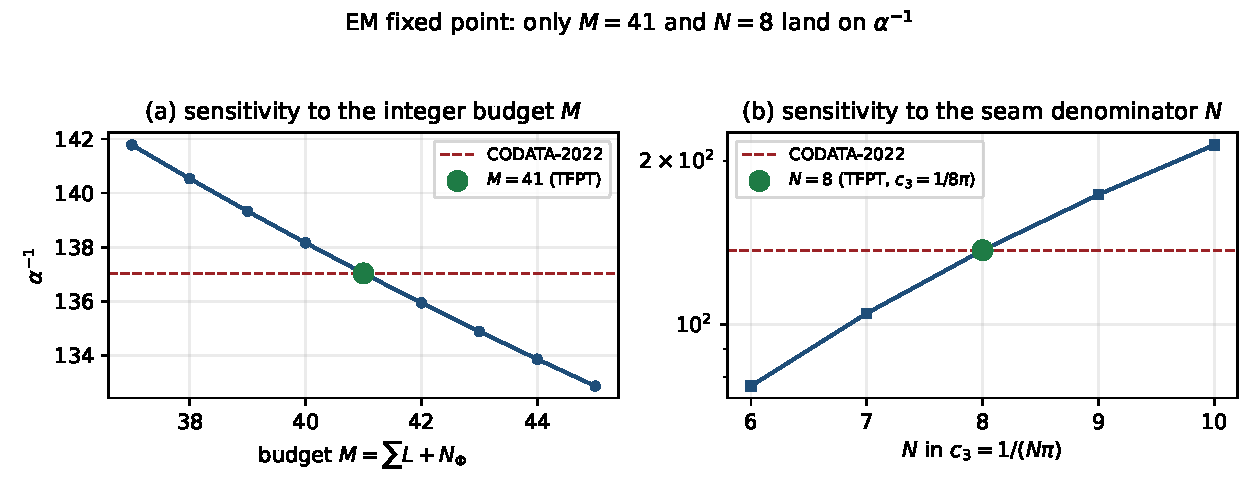
\includegraphics[width=0.92\linewidth]{figures/alpha_ablation.pdf}
\caption{EM-closure ablation (data plot, \texttt{verification/make\_figures.py}). \textbf{(a)} $\ainv$ vs
the integer budget $M$: only $M=41$ lands on CODATA-2022. \textbf{(b)} $\ainv$ vs the seam denominator
$N$ in $\cthree=1/(N\pi)$: only $N=8$ lands. Both integers are fixed elsewhere (flavor budget; rank/$h(D_5)$),
so the equation is not freely tunable to $137.036$.}
\label{fig:ablation}
\end{figure}

% --- ablation 1 ---
\noindent\textbf{(A1) The transport budget $M=\sum L+N_\Phi$} (exponent held at $-\tfrac54$):
\begin{center}\footnotesize\renewcommand{\arraystretch}{1.15}
\begin{tabular}{@{}cccccccc@{}}
\toprule
$M$ & $38$ & $39$ & $40$ & $\mathbf{41}$ & $42$ & $43$ & $44$ \\
\midrule
$\ainv$ & $140.530$ & $139.326$ & $138.162$ & $\mathbf{137.0359992}$ & $135.946$ & $134.890$ & $133.866$ \\
\bottomrule
\end{tabular}
\end{center}
Each unit of $M$ shifts $\ainv$ by $\approx1.09$, so \emph{only} $M=41$ lands on $137.036$. This is a hard
lock --- and $41=10b_1=\sum L+N_\Phi=40+1$ is fixed by the compiler (flavor budget $40$ $+$ one Higgs).
\textbf{Load-bearing.}

% --- ablation 2 ---
\noindent\textbf{(A2) The seam ``8'' in $\cthree=1/(N\pi)$} (here $\dtop=48\cthree^4$ tracks $\cthree$):
\begin{center}\footnotesize\renewcommand{\arraystretch}{1.15}
\begin{tabular}{@{}cccccc@{}}
\toprule
$N$ & $6$ & $7$ & $\mathbf{8}$ & $9$ & $10$ \\
\midrule
$\ainv$ & $76.97$ & $104.85$ & $\mathbf{137.036}$ & $173.53$ & $214.34$ \\
\bottomrule
\end{tabular}
\end{center}
Only $N=8$ --- i.e.\ $\cthree=1/(8\pi)=1/(\operatorname{rank}E_8\cdot\pi)$ --- reproduces $137.036$. The
``8'' is the same one fixed by the bootstrap ($h(D_5)=\operatorname{rank}E_8=\varphi(30)$) and the
Gauss--Bonnet hardening. \textbf{Load-bearing.}

% --- ablation 3 ---
\noindent\textbf{(A3) The carrier discriminant exponent} (at $M=41$, $\cthree=1/(8\pi)$):
\begin{center}\footnotesize\renewcommand{\arraystretch}{1.15}
\begin{tabular}{@{}cccccc@{}}
\toprule
exponent & $-\tfrac14$ & $-\tfrac34$ & $\mathbf{-\tfrac54}$ & $-\tfrac74$ & $-\tfrac94$ \\
\midrule
$\ainv$ & $137.035995$ & $137.035997$ & $\mathbf{137.0359992}$ & $137.036001$ & $137.036003$ \\
\bottomrule
\end{tabular}
\end{center}
The exponent moves only the \emph{seventh} digit; all candidates agree to six. Here $-\tfrac54=q(D_5)$ is
selected, but this is a \emph{fine} selector, not a hard lock. \textbf{Fine (last-digit).}

\begin{keybox}[Ablation verdict --- honest]
The EM fixed point is a \textbf{hard test of two integers} --- the budget $M=41$ and the seam denominator
$8=\operatorname{rank}E_8$, each decisive (a single-unit change misses by $\sim1$ in $\ainv$) --- and a
\textbf{fine test of one norm}, the carrier discriminant exponent $-\tfrac54=q(D_5)$ (seventh digit). The
equation is therefore \emph{not} freely tunable to $137.036$: the two integers that hit it are exactly the
compiler/bootstrap numbers, fixed elsewhere. What it does \emph{not} do is pin the carrier norm strongly
--- that is honest, and it is the right level of claim. \mE
\end{keybox}

% =====================================================================
\section*{Appendix: computational verification}
\addcontentsline{toc}{section}{Appendix: computational verification}
% =====================================================================
The load-bearing identities of this document (marked \mE, \mE, \mE) are re-derived from
$\{\cthree,\gcar\}$ alone and machine-checked by the suite in the repository folder
\texttt{verification/}; the inline tags \texttt{[verification/$\dots$]} point to the exact script.
Relevant here:
\begin{itemize}[leftmargin=1.4em,itemsep=1pt]
\item \texttt{v1\_e8\_glue.py} --- the $\mu_4$ glue ($q(D_5){+}q(A_3){=}2$, $\operatorname{disc}{=}\Z_4$, $240,248$).
\item \texttt{v2\_carrier\_pascal.py} --- $\gcar{=}5$, $16{=}1{+}5{+}10$, $\Nfam,\Oadm,b_1$.
\item \texttt{v3\_em\_alpha.py} --- the EM fixed point $\ainv{=}137.0359992168$ (existence/uniqueness, ablation).
\item \texttt{v4\_flavor\_matrix.py} --- $R$ with $\det{=}8$, minors $\{2,3,5\}$, $\sum L{=}40$.
\item \texttt{v7\_gravity\_cosmo.py} --- scalaron $\cthree^7$, $\Lambda$/$A_s$ readouts.
\end{itemize}
Run \texttt{python verification/run\_all.py} (needs \texttt{mpmath, numpy, sympy}); it exits $0$ iff all
checks pass. Full map: \texttt{verification/README.md}.

% ---------------------------------------------------------------------
%  tfpt_references.tex -- shared "external works built upon" appendix.
%  Single source (tex-artefacts/), \input near the end of the math-heavy
%  documents.  Plain LaTeX only (no document-specific macros), so it
%  compiles unchanged in every paper that imports it.
%  Every entry below was web-verified (journal, volume, year / arXiv id).
%  TFPT's discrete core is self-contained and machine-checked; the entries
%  here are the established mathematics its continuum/AQFT and gravity
%  BRIDGES build on, collected for the reader (the active papers refer to
%  these results by author name in the text).
% ---------------------------------------------------------------------
\section*{External works built upon}
\small
\noindent
The TFPT discrete core (the two axioms, the $E_8$ glue, the integer skeleton) is
self-contained and machine-checked. Its \emph{bridges} to continuum/AQFT physics, to
gravity and to the lattice/singularity picture build on established mathematics, listed
here by topic; the body refers to these by author name.

\paragraph{Modular theory and algebraic quantum field theory.}
\begin{itemize}\setlength\itemsep{1.5pt}
\item M.~Takesaki, \textit{Tomita's Theory of Modular Hilbert Algebras and its
  Applications}, Lecture Notes in Math.\ \textbf{128}, Springer (1970).
\item J.~J.~Bisognano, E.~H.~Wichmann, \textit{On the duality condition for a Hermitian
  scalar field} / \textit{for quantum fields}, J.~Math.\ Phys.\ \textbf{16} (1975)
  985--1007; \textbf{17} (1976) 303--321.
\item K.~Osterwalder, R.~Schrader, \textit{Axioms for Euclidean Green's functions} I, II,
  Comm.\ Math.\ Phys.\ \textbf{31} (1973) 83--112; \textbf{42} (1975) 281--305.
\item S.~Doplicher, R.~Haag, J.~E.~Roberts, \textit{Local observables and particle
  statistics} I, II, Comm.\ Math.\ Phys.\ \textbf{23} (1971) 199--230; \textbf{35} (1974)
  49--85.
\item R.~Haag, \textit{Quantum field theories with composite particles and asymptotic
  conditions}, Phys.\ Rev.\ \textbf{112} (1958) 669--673; D.~Ruelle, \textit{On the
  asymptotic condition in quantum field theory}, Helv.\ Phys.\ Acta \textbf{35} (1962)
  147--163.
\item R.~Longo, \textit{Index of subfactors and statistics of quantum fields} I, II, Comm.\
  Math.\ Phys.\ \textbf{126} (1989) 217--247; \textbf{130} (1990) 285--309.
\item Y.~Kawahigashi, R.~Longo, M.~M\"uger, \textit{Multi-interval subfactors and modularity
  of representations in conformal field theory}, Comm.\ Math.\ Phys.\ \textbf{219} (2001)
  631--669.
\end{itemize}

\paragraph{Conformal nets, vertex operator algebras and lattice constructions.}
\begin{itemize}\setlength\itemsep{1.5pt}
\item I.~B.~Frenkel, V.~G.~Kac, \textit{Basic representations of affine Lie algebras and
  dual resonance models}, Invent.\ Math.\ \textbf{62} (1980) 23--66; G.~Segal,
  \textit{Unitary representations of some infinite-dimensional groups}, Comm.\ Math.\ Phys.\
  \textbf{80} (1981) 301--342.
\item T.~J.~Osborne, A.~Stottmeister, \textit{Conformal field theory from lattice
  fermions}, Comm.\ Math.\ Phys.\ \textbf{398} (2023) 219--289,
  \texttt{arXiv:2107.13834}, \texttt{doi:10.1007/s00220-022-04521-8}.  (This is the
  seam scaling-limit theorem the TFPT continuum leg cites --- the Koo--Saleur $\to$
  Virasoro convergence, $c=\tfrac12$, and the smeared WZW-current Theorem~5.1.  The
  internal TFPT code-token ``MMST'' and the legacy claim-ids \texttt{SEAM.MMST.*} /
  filenames \texttt{v*\_mmst\_*} denote \emph{this} Osborne--Stottmeister theorem.)
\item V.~Morinelli, G.~Morsella, A.~Stottmeister, Y.~Tanimoto, \textit{Scaling limits
  of lattice quantum fields by wavelets}, Comm.\ Math.\ Phys.\ \textbf{387} (2021)
  299--360, \texttt{arXiv:2010.11121}, \texttt{doi:10.1007/s00220-021-04152-5}; and
  \textit{Operator-algebraic renormalization and wavelets}, Phys.\ Rev.\ Lett.\
  \textbf{127} (2021) 230601.  (The operator-algebraic (wavelet/Wilson--Kadanoff)
  renormalization \emph{framework} the Osborne--Stottmeister theorem above builds on.)
\item M.~S.~Adamo, Y.~Moriwaki, Y.~Tanimoto, \textit{Osterwalder--Schrader axioms for
  unitary full vertex operator algebras}, \texttt{arXiv:2407.18222} (2024).
\item M.~S.~Adamo, L.~Giorgetti, Y.~Tanimoto, \textit{Rational and non-rational
  two-dimensional conformal field theories arising from lattices}, \texttt{arXiv:2506.01008}
  (2025); \textit{Representations of conformal nets associated with infinite-dimensional
  groups}, \texttt{arXiv:2508.07109} (2025).
\item P.~Naaijkens, D.~Penneys, B.~Wallick, \textit{(commuting-projector reflection
  positivity / LTO-RP)}, \texttt{arXiv:2605.10693}.
\end{itemize}

\paragraph{Lattices and quadratic forms.}
\begin{itemize}\setlength\itemsep{1.5pt}
\item J.~H.~Conway, N.~J.~A.~Sloane, \textit{Sphere Packings, Lattices and Groups}, 3rd ed.,
  Grundlehren der math.\ Wiss.\ \textbf{290}, Springer (1999).
\item C.~L.~Siegel, \textit{\"Uber die analytische Theorie der quadratischen Formen}
  (the Minkowski--Siegel mass formula), Ann.\ of Math.\ \textbf{36} (1935) 527--606.
\end{itemize}

\paragraph{Singularities and geometry.}
\begin{itemize}\setlength\itemsep{1.5pt}
\item E.~Brieskorn, \textit{Beispiele zur Differentialtopologie von Singularit\"aten},
  Invent.\ Math.\ \textbf{2} (1966) 1--14.
\item J.~Milnor, \textit{Singular Points of Complex Hypersurfaces}, Ann.\ of Math.\ Studies
  \textbf{61}, Princeton Univ.\ Press (1968).
\end{itemize}

\paragraph{Spectral geometry, gravity and thermal time.}
\begin{itemize}\setlength\itemsep{1.5pt}
\item A.~H.~Chamseddine, A.~Connes, \textit{The spectral action principle}, Comm.\ Math.\
  Phys.\ \textbf{186} (1997) 731--750.
\item A.~Connes, C.~Rovelli, \textit{Von Neumann algebra automorphisms and
  time--thermodynamics relation in general covariant quantum theories}, Class.\ Quantum
  Grav.\ \textbf{11} (1994) 2899--2918.
\item R.~M.~Wald, \textit{Black hole entropy is the Noether charge}, Phys.\ Rev.\ D
  \textbf{48} (1993) R3427--R3431.
\item H.~Casini, M.~Huerta, R.~C.~Myers, \textit{Towards a derivation of holographic
  entanglement entropy}, JHEP \textbf{05} (2011) 036, \texttt{arXiv:1102.0440}.
\end{itemize}
\normalsize


\end{document}
